% Options for packages loaded elsewhere
\PassOptionsToPackage{unicode}{hyperref}
\PassOptionsToPackage{hyphens}{url}
\PassOptionsToPackage{dvipsnames,svgnames,x11names}{xcolor}
%
\documentclass[
  letterpaper,
]{book}

\usepackage{amsmath,amssymb}
\usepackage{iftex}
\ifPDFTeX
  \usepackage[T1]{fontenc}
  \usepackage[utf8]{inputenc}
  \usepackage{textcomp} % provide euro and other symbols
\else % if luatex or xetex
  \usepackage{unicode-math}
  \defaultfontfeatures{Scale=MatchLowercase}
  \defaultfontfeatures[\rmfamily]{Ligatures=TeX,Scale=1}
\fi
\usepackage{lmodern}
\ifPDFTeX\else  
    % xetex/luatex font selection
\fi
% Use upquote if available, for straight quotes in verbatim environments
\IfFileExists{upquote.sty}{\usepackage{upquote}}{}
\IfFileExists{microtype.sty}{% use microtype if available
  \usepackage[]{microtype}
  \UseMicrotypeSet[protrusion]{basicmath} % disable protrusion for tt fonts
}{}
\makeatletter
\@ifundefined{KOMAClassName}{% if non-KOMA class
  \IfFileExists{parskip.sty}{%
    \usepackage{parskip}
  }{% else
    \setlength{\parindent}{0pt}
    \setlength{\parskip}{6pt plus 2pt minus 1pt}}
}{% if KOMA class
  \KOMAoptions{parskip=half}}
\makeatother
\usepackage{xcolor}
\usepackage[a4paper,left=1.25in,right=1.25in,top=1.00in,bottom=1.00in,textwidth=5.25in,textheight=8.75in]{geometry}
\setlength{\emergencystretch}{3em} % prevent overfull lines
\setcounter{secnumdepth}{5}
% Make \paragraph and \subparagraph free-standing
\makeatletter
\ifx\paragraph\undefined\else
  \let\oldparagraph\paragraph
  \renewcommand{\paragraph}{
    \@ifstar
      \xxxParagraphStar
      \xxxParagraphNoStar
  }
  \newcommand{\xxxParagraphStar}[1]{\oldparagraph*{#1}\mbox{}}
  \newcommand{\xxxParagraphNoStar}[1]{\oldparagraph{#1}\mbox{}}
\fi
\ifx\subparagraph\undefined\else
  \let\oldsubparagraph\subparagraph
  \renewcommand{\subparagraph}{
    \@ifstar
      \xxxSubParagraphStar
      \xxxSubParagraphNoStar
  }
  \newcommand{\xxxSubParagraphStar}[1]{\oldsubparagraph*{#1}\mbox{}}
  \newcommand{\xxxSubParagraphNoStar}[1]{\oldsubparagraph{#1}\mbox{}}
\fi
\makeatother


\providecommand{\tightlist}{%
  \setlength{\itemsep}{0pt}\setlength{\parskip}{0pt}}\usepackage{longtable,booktabs,array}
\usepackage{calc} % for calculating minipage widths
% Correct order of tables after \paragraph or \subparagraph
\usepackage{etoolbox}
\makeatletter
\patchcmd\longtable{\par}{\if@noskipsec\mbox{}\fi\par}{}{}
\makeatother
% Allow footnotes in longtable head/foot
\IfFileExists{footnotehyper.sty}{\usepackage{footnotehyper}}{\usepackage{footnote}}
\makesavenoteenv{longtable}
\usepackage{graphicx}
\makeatletter
\newsavebox\pandoc@box
\newcommand*\pandocbounded[1]{% scales image to fit in text height/width
  \sbox\pandoc@box{#1}%
  \Gscale@div\@tempa{\textheight}{\dimexpr\ht\pandoc@box+\dp\pandoc@box\relax}%
  \Gscale@div\@tempb{\linewidth}{\wd\pandoc@box}%
  \ifdim\@tempb\p@<\@tempa\p@\let\@tempa\@tempb\fi% select the smaller of both
  \ifdim\@tempa\p@<\p@\scalebox{\@tempa}{\usebox\pandoc@box}%
  \else\usebox{\pandoc@box}%
  \fi%
}
% Set default figure placement to htbp
\def\fps@figure{htbp}
\makeatother
% definitions for citeproc citations
\NewDocumentCommand\citeproctext{}{}
\NewDocumentCommand\citeproc{mm}{%
  \begingroup\def\citeproctext{#2}\cite{#1}\endgroup}
\makeatletter
 % allow citations to break across lines
 \let\@cite@ofmt\@firstofone
 % avoid brackets around text for \cite:
 \def\@biblabel#1{}
 \def\@cite#1#2{{#1\if@tempswa , #2\fi}}
\makeatother
\newlength{\cslhangindent}
\setlength{\cslhangindent}{1.5em}
\newlength{\csllabelwidth}
\setlength{\csllabelwidth}{3em}
\newenvironment{CSLReferences}[2] % #1 hanging-indent, #2 entry-spacing
 {\begin{list}{}{%
  \setlength{\itemindent}{0pt}
  \setlength{\leftmargin}{0pt}
  \setlength{\parsep}{0pt}
  % turn on hanging indent if param 1 is 1
  \ifodd #1
   \setlength{\leftmargin}{\cslhangindent}
   \setlength{\itemindent}{-1\cslhangindent}
  \fi
  % set entry spacing
  \setlength{\itemsep}{#2\baselineskip}}}
 {\end{list}}
\usepackage{calc}
\newcommand{\CSLBlock}[1]{\hfill\break\parbox[t]{\linewidth}{\strut\ignorespaces#1\strut}}
\newcommand{\CSLLeftMargin}[1]{\parbox[t]{\csllabelwidth}{\strut#1\strut}}
\newcommand{\CSLRightInline}[1]{\parbox[t]{\linewidth - \csllabelwidth}{\strut#1\strut}}
\newcommand{\CSLIndent}[1]{\hspace{\cslhangindent}#1}

\makeatletter
\@ifpackageloaded{bookmark}{}{\usepackage{bookmark}}
\makeatother
\makeatletter
\@ifpackageloaded{caption}{}{\usepackage{caption}}
\AtBeginDocument{%
\ifdefined\contentsname
  \renewcommand*\contentsname{Table of contents}
\else
  \newcommand\contentsname{Table of contents}
\fi
\ifdefined\listfigurename
  \renewcommand*\listfigurename{List of Figures}
\else
  \newcommand\listfigurename{List of Figures}
\fi
\ifdefined\listtablename
  \renewcommand*\listtablename{List of Tables}
\else
  \newcommand\listtablename{List of Tables}
\fi
\ifdefined\figurename
  \renewcommand*\figurename{Figure}
\else
  \newcommand\figurename{Figure}
\fi
\ifdefined\tablename
  \renewcommand*\tablename{Table}
\else
  \newcommand\tablename{Table}
\fi
}
\@ifpackageloaded{float}{}{\usepackage{float}}
\floatstyle{ruled}
\@ifundefined{c@chapter}{\newfloat{codelisting}{h}{lop}}{\newfloat{codelisting}{h}{lop}[chapter]}
\floatname{codelisting}{Listing}
\newcommand*\listoflistings{\listof{codelisting}{List of Listings}}
\makeatother
\makeatletter
\makeatother
\makeatletter
\@ifpackageloaded{caption}{}{\usepackage{caption}}
\@ifpackageloaded{subcaption}{}{\usepackage{subcaption}}
\makeatother

\usepackage{bookmark}

\IfFileExists{xurl.sty}{\usepackage{xurl}}{} % add URL line breaks if available
\urlstyle{same} % disable monospaced font for URLs
\hypersetup{
  pdftitle={Grundlagen des Sozialmanagements},
  colorlinks=true,
  linkcolor={Maroon},
  filecolor={Maroon},
  citecolor={Blue},
  urlcolor={Blue},
  pdfcreator={LaTeX via pandoc}}


\title{Grundlagen des Sozialmanagements}
\usepackage{etoolbox}
\makeatletter
\providecommand{\subtitle}[1]{% add subtitle to \maketitle
  \apptocmd{\@title}{\par {\large #1 \par}}{}{}
}
\makeatother
\subtitle{Begriffe - Konzepte - Ansätze}
\author{}
\date{}

\begin{document}
\frontmatter
\maketitle

\renewcommand*\contentsname{Table of contents}
{
\hypersetup{linkcolor=}
\setcounter{tocdepth}{2}
\tableofcontents
}

\mainmatter
\bookmarksetup{startatroot}

\chapter*{Über das OER Textbook}\label{uxfcber-das-oer-textbook}
\addcontentsline{toc}{chapter}{Über das OER Textbook}

\markboth{Über das OER Textbook}{Über das OER Textbook}

Dieses Open Educational Textbook ist im Rahmen des Moduls
\emph{Grundlagen des Sozialmanagements} an der
\href{https://www.fh-dresden.de}{Fachhochschule Dresden} im
Bachelorstudiengang \emph{Sozialpädagogik und -management} entstanden.
Aktuell wird es an der \href{https://www.hs-nordhausen.de}{Hochschule
Nordhausen} im Bachelorstudiengang \emph{Sozialmanagement} im
gleichnamigen Studienbereich weitergeführt. Das Textbook stellt
einerseits eine Einführung in sozial- und -betriebswirtschaftliche
Grundlagen, die Gestaltung und das Management von Organisationen in der
Sozialwirtschaft dar. Andererseits wird ausführlich auch auf das
organisationsbezogene Management in sowie die Finanzierung von
Sozialunternehmen sowie auf ausgewählte Managementkonzept in der
Sozialwirtschaft eingegangen. Das Lehrbuch entstand vor dem Hintergrund
von COVID-19 und im Bemühen um eine verstärkte Zusammenarbeit von
Studierenden, Lehrenden, Forschenden und Praktiker*innen im Sozialwesen
und Gesundheitsbereich sowie angrenzender Disziplinen und Feldern Dieses
\href{https://de.wikipedia.org/wiki/Open_Educational_Resources}{Open
Educational Resource} Textbook versteht sich als ein Wissensfundus, der
kontinuierlich ergänzt, diskutiert und weiterentwickelt wird.

\textbf{Dieses Buch wurde zuletzt gerendert am 2025-03-28.}

\section*{Lizenz}\label{lizenz}
\addcontentsline{toc}{section}{Lizenz}

\markright{Lizenz}

Dieses Buch ist kostenlos verfügbar und unter der
\href{https://creativecommons.org/licenses/by-nc-sa/4.0/}{CC BY-NC-ND
4.0 International License} lizenziert. Das bedeutet, dass das Buch
geteilt und weitergegeben werden kann, solange die Autor*innen
angemessen genannt und eventuelle geringfügige Änderungen entsprechend
gekennzeichnet werden. Geänderte Versionen, die den Inhalt remixen oder
modifizieren, dürfen jedoch nicht verbreitet werden.

\section*{Empfohlene Zitierweise (APA
7th)}\label{empfohlene-zitierweise-apa-7th}
\addcontentsline{toc}{section}{Empfohlene Zitierweise (APA 7th)}

\markright{Empfohlene Zitierweise (APA 7th)}

Arnold, M. (2020). \emph{Grundlagen des Sozialmanagements: Ein Open
Educational Textbook} (2. Aufl.). Hochschule Nordhausen.
https://doi.org/XXX.

\section*{Acknowledgement}\label{acknowledgement}
\addcontentsline{toc}{section}{Acknowledgement}

\markright{Acknowledgement}

Zur Entstehung dieses OER Textbooks haben insbesondere die folgenden
Personen beigetragen: Die Korrektur einzelner Textabschnitte haben
insbesondere Frau Sandy Albrecht, Frau Lisa Jurke, Herr Tony Krüger,
Frau Cindy Rasokat, Frau Jacqueline Seubert und Frau Tina Steinborn
unterstützt. Zu großem Dank bin ich speziell Herrn Stefan Jung
verpflichtet, der in mühseliger Kleinarbeit ein Lektorat am Manuskript
der ersten Auflage durchgeführt hat. Die Entstehung der zweiten Auflage
hat Hr. Gustavo Tadra Waldmann unterstützt.

\part{Grundlagen}

\chapter{Einführung}\label{einfuehrung}

In diesem einführenden Kapitel wird zunächst anhand einer sog.
Fachlandkarte auf das Themenfeld Sozialmanagement und Sozialwirtschaft
eingegangen. Im Anschluss folgt ein Überblick zur Geschichte und
statistischen Einordnung dieses Arbeitsfeldes bzw. gesellschaftlichen
Sektors, den wir als Sozialwirtschaft bezeichnen. Außerdem müssen
verschiedene Begriffsabgrenzungen vorgenommen werden, wie z. B. zwischen
\emph{Sozialmanagement} und \emph{Non-Profit-Management} (vgl. z. B.
Armin Wöhrle 2017), und auch muss darauf eingegangen werden, was
Organisationen der Sozialwirtschaft von Non-Profit-Organisationen
unterscheidet.

Das Sozialmanagement lässt sich anhand einer Fachlandkarte
untergliedern. Eine Fachlandkarte wird in der Hochschuldidaktik genutzt,
um komplexe Zusammenhänge übersichtlich darzustellen und um damit
Lernenden in ein komplexes Arbeits-, Themen- und Forschungsfeld
einzuführen (vgl. z. B. Ritter-Mamczek 2016). Im Folgenden wird der
Versuch unternommen, auf einer „Schatzkarte'' die verschiedenen
Provinzen des
\href{https://de.wikipedia.org/wiki/Sozialmanagement}{Sozialmanagements}
zusammenzufassen und zu entdecken (vgl. \hyperref[figure11]{Abb. 1.1}).

\begin{figure}

\pandocbounded{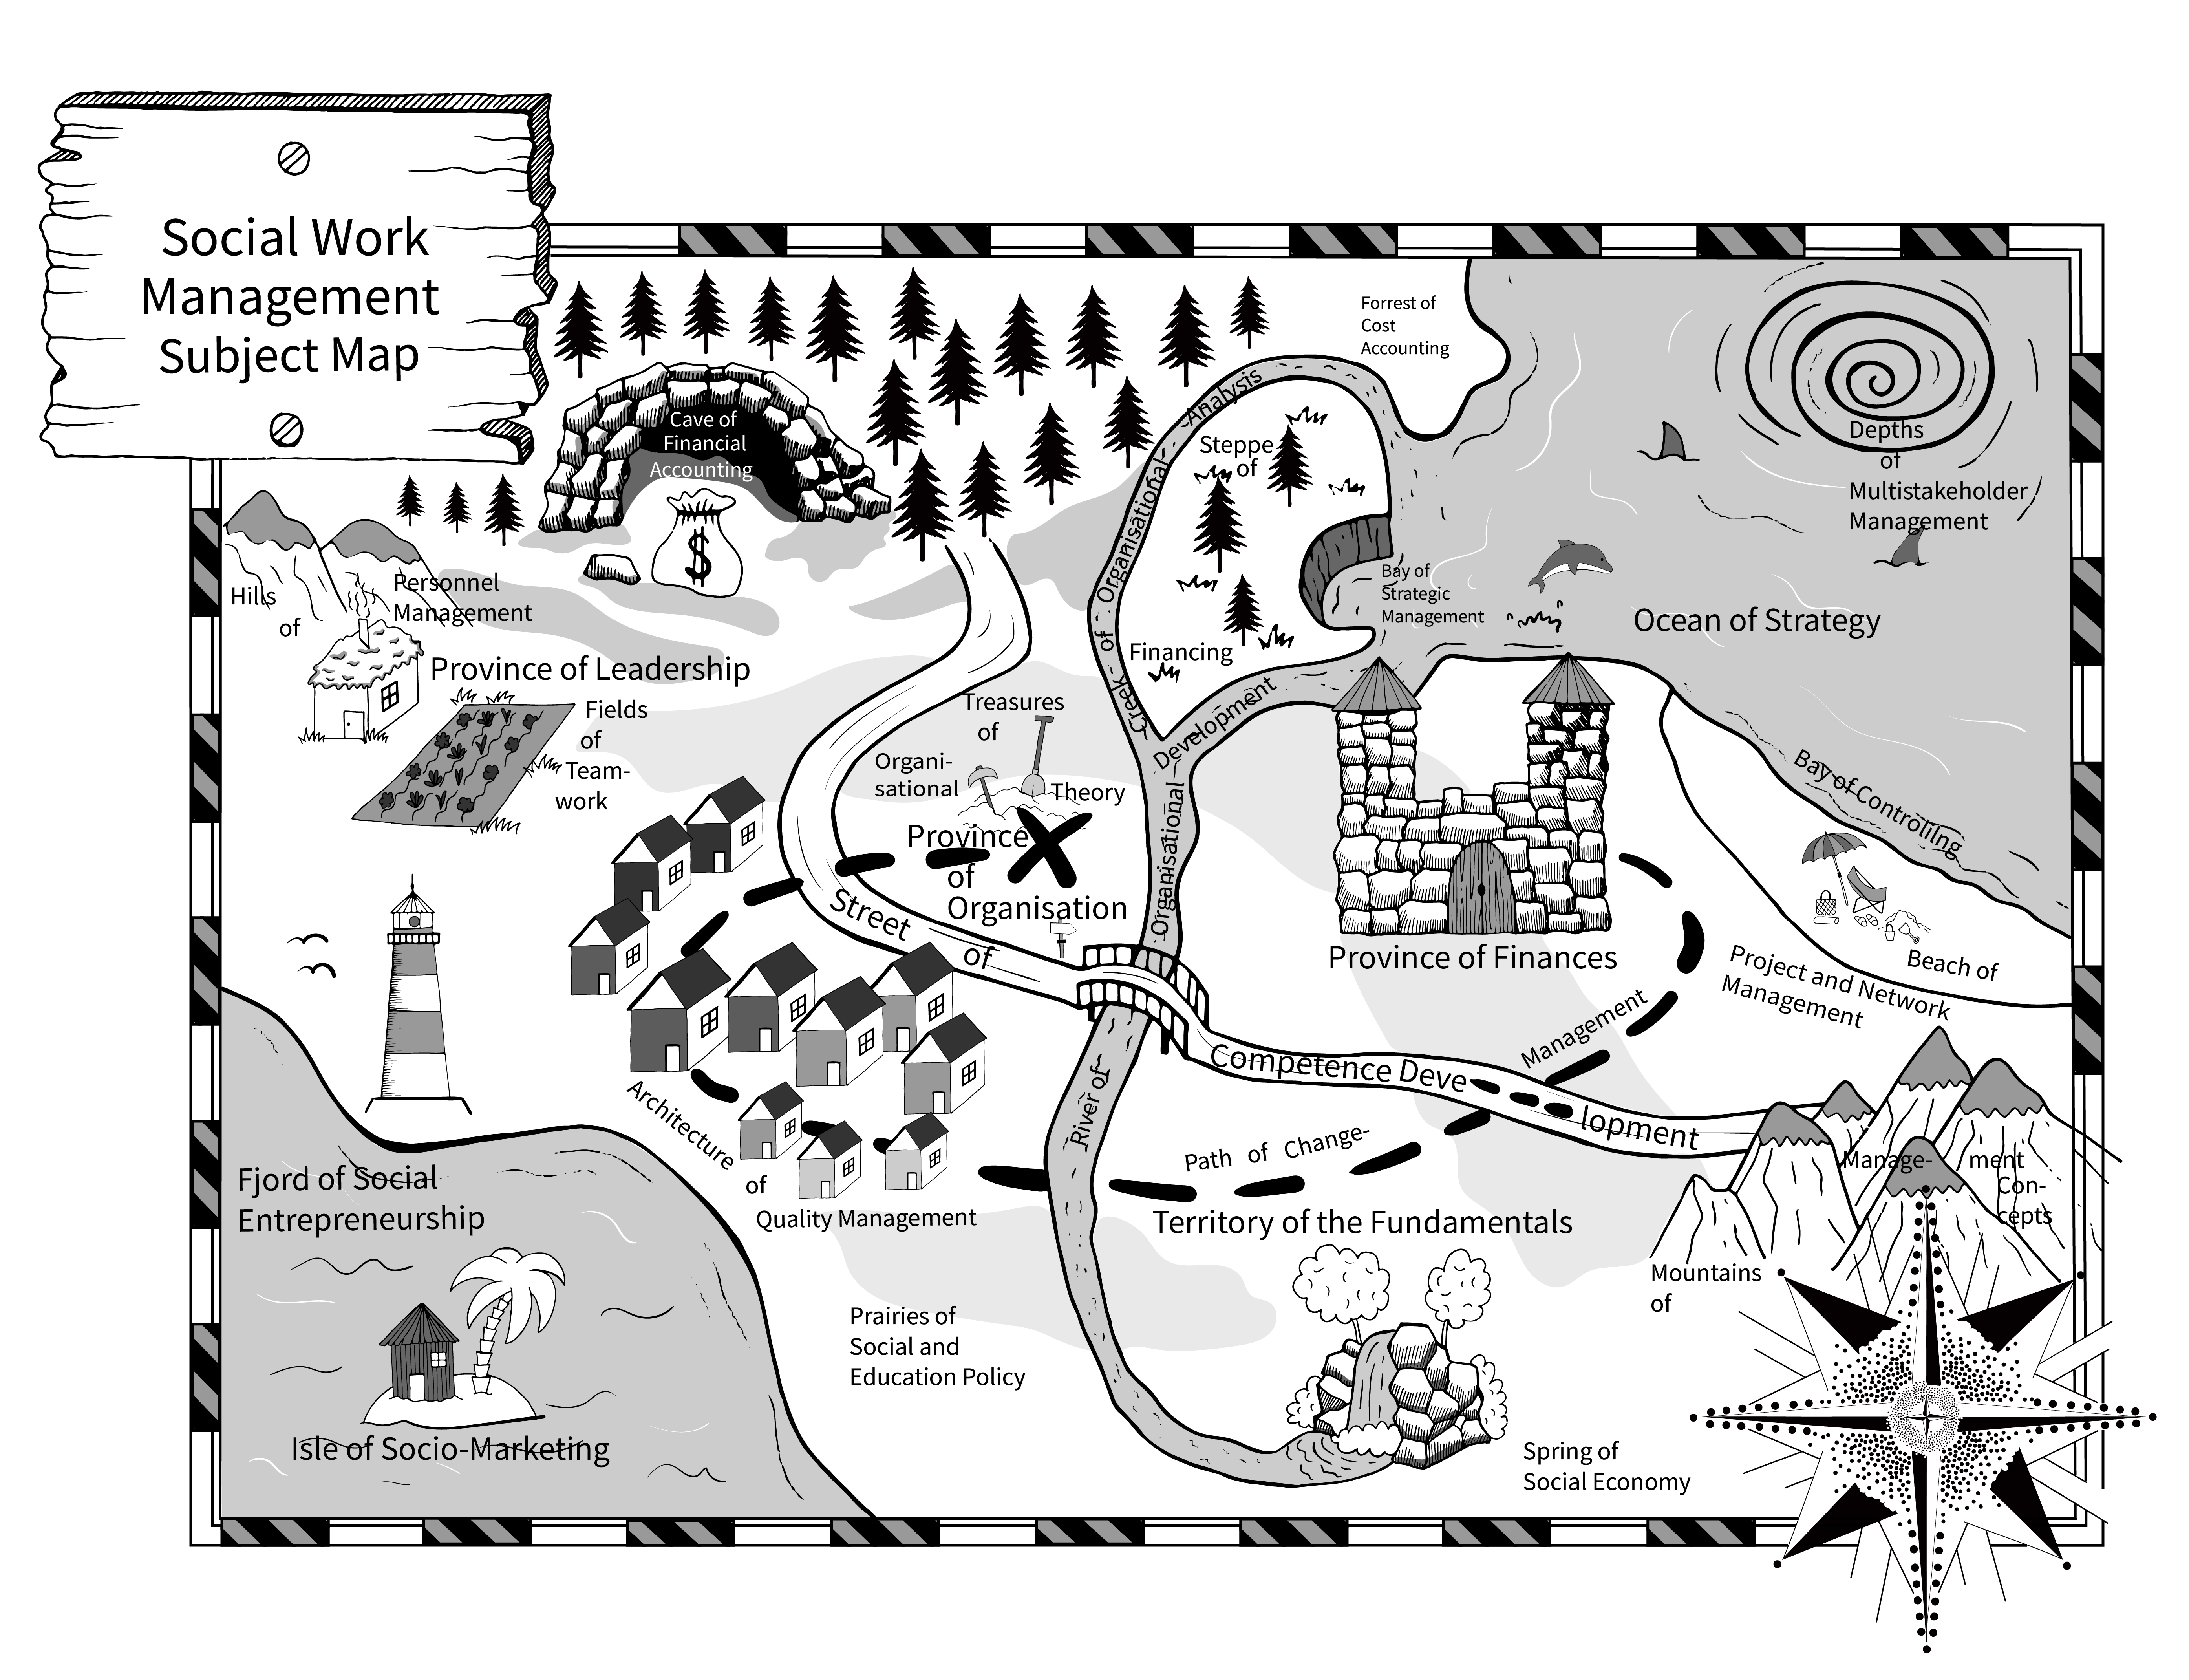
\includegraphics[keepaspectratio]{images/figure11.png}} \hfill{}

\caption{Abb. 1.1: Fachlandkarte Sozialmanagement (Arnold 2022b, CC--BY
4.0)}

\end{figure}%

Im Bild ist das \emph{Territorium der Grundlagen} zu sehen. Hier
befinden wir uns an der Quelle der Sozialwirtschaft, d.~h. es gilt die
\emph{sozialpolitischen} und \emph{bildungspolitischen
Rahmenbedingungen} und verschiedene \emph{Managementkonzepte}
kennenzulernen, wie soziale Organisation geleitet, geführt und gestaltet
werden können. Links oben im Bild ist die Höhle der
\emph{Finanzbuchhaltung} zu sehen, die sich mit der Verwaltung der
verfügbaren Finanzmittel beschäftigt. Im Wald der \emph{Kosten- und
Leistungsrechnung} können wir uns zudem einen Überblick darüber
verschaffen, wie wirtschaftlich unsere Organisation arbeitet.

Darüber hinaus ist in der Mitte des Bilds die Provinz der Organisation
zu erkennen. Man braucht ein grundlegendes Wissen über die
Organisationstheorie, z. B. darüber wie \emph{Organisationen in der
Sozialwirtschaft} aufgebaut sind, wie sie finanziert werden und wie sie
letztlich funktionieren. Dann gibt es die Provinz der Finanzen, wo es
neben der Kosten- und Leistungsrechnung und Buchführung um die Frage der
\emph{Finanzierung} geht. In diesem Zusammenhang muss ein Überblick über
die verschiedenen Finanzquellen gewonnen werden (wie z. B.
Leistungsentgelte oder Spenden). Schließlich gibt es noch am linken Rand
die Provinz des \emph{Leaderships}, wo man sich u. a. die Frage stellt,
was adäquate Mittel, Werkzeuge und Instrumente darstellen, um Führung
und Personalentwicklung innerhalb sozialer Organisationen zu gestalten.

An den Rändern der Karte sehen wir links unten das \emph{Social
Entrepreneurship} und die Insel des \emph{Sozio-Marketings}. Dort sind
alle Aufgaben- und Themenstellungen versammelt, die sich mit der
Unternehmensgründung bzw. dem Marketing beschäftigen. Darüber hinaus ist
am rechten oberen Rand der Landkarte der Ozean der Strategie abgebildet.
Im Rahmen des Sozialmanagements muss sich daher auch mit den
verschiedenen Aspekte und \emph{Grundlagen des strategischen
Managements} auseinandergesetzt werden, z. B. wie man Organisationen
langfristig leiten, gestalten und steuern kann. In der Bucht des
\emph{Controllings} kann man sich sprichwörtlich an den Strand setzen,
wo man sich das \emph{Projekt- und Netzwerkmanagement} zu Gemüte führen
kann, was natürlich auch eine wesentliche Grundkompetenz dafür
darstellt, um in sozialen Organisationen zu arbeiten.

Kurzum sind in dieser Fachlandkarte verschiedene Arbeits- und
Themenfelder zu finden, die in diesem Grundlagenlehrbuch vorgestellt und
vertieft werden. Der Fokus dieses OER Textbuchs liegt allerdings auf
einer Einführung in die sozial- und betriebswirtschaftlichen Grundlagen,
dem organisationsbezogenen Management sowie den Managementansätzen für
das Sozialmanagement liegen.\footnote{Für eine ausführliche Darstellung
  der wichtigsten Entwicklungsschritte vgl. z. B..Wöhrle, A. (2011).
  Sozialwirtschaft. In H. Thiersch, \& H. U. Otto (2011), \emph{Handbuch
  Soziale Arbeit}. \emph{Grundlagen der Sozialarbeit und
  Sozialpädagogik} (S. 1562-1570, 5. Aufl.). München: Ernst Reinhardt.
  https://doi.org/10.2378/ot4a.art145}

\section{Geschichte der Sozialwirtschaft}\label{geschichte}

\subsection[Die Anfänge der Sozialwirtschaft]{\texorpdfstring{Die
Anfänge der
Sozialwirtschaft\footnote{Für eine ausführliche Darstellung der
  wichtigsten Entwicklungsschritte vgl. z. B..Wöhrle, A. (2011).
  Sozialwirtschaft. In H. Thiersch, \& H. U. Otto (2011), \emph{Handbuch
  Soziale Arbeit}. \emph{Grundlagen der Sozialarbeit und
  Sozialpädagogik} (S. 1562-1570, 5. Aufl.). München: Ernst Reinhardt.
  https://doi.org/10.2378/ot4a.art145}}{Die Anfänge der Sozialwirtschaft}}\label{die-anfaenge-der-sozialwirtschaft}

Ein Ausflug in die Geschichte des Sozialmanagements bzw. der
Sozialwirtschaft ist notwendig, nicht nur um zu verstehen, wie sich
alles entwickelt hat, sondern auch um viele der aktuell diskutierten
Fragen rund um den Sozialstaat besser nachvollziehen zu können. Wir
beginnen in der Neuzeit, insbesondere in Frankreich, mit der ersten
Erwähnung bzw. der ersten theoretischen Auseinandersetzung mit
sozialwirtschaftlichen Grundlagen, wie z. B. der
\href{https://de.wikipedia.org/wiki/Katholische_Soziallehre}{katholischen
Soziallehre}. In den
\href{https://de.wikipedia.org/wiki/Sozialenzyklika}{päpstlichen
Sozialenzykliken} wurden bspw. Gedanken entwickelt, die später in Form
des rechtlich verbindlichen
\href{https://www.bpb.de/kurz-knapp/lexika/pocket-europa/16951/subsidiaritaetsprinzip/}{Subsidiaritätsprinzips}
weiterentwickelt wurden und mittlerweile die Rahmenbedingungen für viele
entwickelten Sozialökonomien (wie z. B. für die deutsche
\href{https://www.bpb.de/kurz-knapp/lexika/lexikon-der-wirtschaft/20642/soziale-marktwirtschaft/}{Soziale
Marktwirtschaft}) darstellen. Zur etwa gleichen Zeit ist
\href{https://de.wikipedia.org/wiki/L\%C3\%A9on_Walras}{Léon Walras} im
Rahmen seiner
\href{https://de.wikipedia.org/wiki/Walrasianisches_allgemeines_Gleichgewichtsmodell}{allgemeinen
Gleichgewichtstheorie} der Frage nachgegangen, wie Grund und Boden denn
verstaatlicht werden können. Wenn mit einer Verstaatlichung zwar Steuern
vermieden werden, so könnte seiner Meinung nach doch zumindest die
Produktion gesteigert werden. Dies soll und kann an dieser Stelle keine
vollständige Darstellung der geschichtlichen Grundlagen darstellen. Wir
wollen es bei diesen Beispielen belassen. Festzuhalten ist aber, dass
all diese verschiedene Grundlagen das „soziale Wirtschaften'' (vgl. z.
B. Beck et al. 2013) in unseren heutigen (post-)modernen Gesellschaften
zu beschreiben und zu verstehen verhelfen.

\subsection{Gründung von Genossenschaften, Diakonie und die
Bismarck'schen Gesetze}\label{gruendung}

Wenig später ist es zur Etablierung bzw. Entwicklung des
Genossenschaftswesens gekommen.
\href{https://de.wikipedia.org/wiki/Genossenschaft}{Genossenschaften}
waren ursprünglich nicht \emph{per se} als sozial-gemeinnützige
Einrichtungen ins Leben gerufen, sondern sind vielmehr dafür gegründet
worden, einen Zusammenschluss oder Verbund von Personen und
Einrichtungen zur wirtschaftlichen und/oder sozialen Förderung ihrer
Mitglieder ins Leben zu rufen, z. B. wie Raiffeisen für hilfsbedürftige
Landarbeiter oder die Volksbanken im Bankenwesen. In diesem Zusammenhang
wurden wichtige Prinzipien entwickelt, wie z. B. die
Selbstverantwortung, Selbsthilfe und Selbstverwaltung innerhalb von
Genossenschaften, die in den letzten Jahren wieder verstärkt in der
Organisationsforschung diskutiert wurden. Später kam es dann
insbesondere im Bereich der konfessionellen Trägerschaften im
\href{https://www.diakonie.de/}{Diakonie}- und
\href{https://www.caritas.de/}{Caritaswesen} zur Gründung von
Einrichtungen, die sich speziell um die Notlagen von Menschen gekümmert
haben. Beispielhaft sei hier die Gründung der ersten Stadtmission in
Deutschland von
\href{https://de.wikipedia.org/wiki/Johann_Hinrich_Wichern}{Johann
Hinrich Wichern} in Hamburg genannt. Es sollte nicht unerwähnt bleiben,
dass am Ende des 19. Jahrhunderts die
\href{https://www.bpb.de/themen/soziale-lage/rentenpolitik/289619/bismarcks-sozialgesetze/}{Bismarcksche
Sozialgesetze} eine Innovation des sozialstaatlichen Denkens darstellte
und ein wichtiges Fundament für das
\href{https://de.wikipedia.org/wiki/Sozialversicherung}{Sozialversicherungswesen}
und die Etablierung bzw. Festsetzung des
\href{https://www.bpb.de/themen/gesundheit/gesundheitspolitik/252319/das-solidarprinzip/}{Solidarprinzips}
bildete.

\subsection{Paradigmenwechsel in der Finanzierung der
Sozialwirtschaft}\label{paradigmenwechsel}

Im 20. Jahrhundert stand lange Zeit zunächst das Prinzip der
Vollkostendeckung bzw. „Selbstkostendeckung'' (Mroß 2017) im
Vordergrund, d.~h. alle Einrichtungen, die
\href{https://www.gesetze-im-internet.de/ao_1977/__52.html\#:~:text=(1)\%20Eine\%20K\%C3\%B6rperschaft\%20verfolgt\%20gemeinn\%C3\%BCtzige,sittlichem\%20Gebiet\%20selbstlos\%20zu\%20f\%C3\%B6rdern.}{gemeinnützigeZwecke}
verfolgt haben und als
\href{https://de.wikipedia.org/wiki/Leistungserbringer}{Leistungserbringer}
aufgetreten sind, haben sämtliche notwendigen finanziellen Mittel vom
Staat vollständig refinanziert bekommen. Mitte der 1970er Jahre ist aus
der Kritik am „Versorgungs- oder Wohlfahrtsstaat'' das Anliegen
entstanden, dass man insbesondere diesen Bereich der Sozialwirtschaft
und letztlich auch das Sozialmanagement stärker professionalisieren
sollte.

\subsection{Etablierung der ersten Studiengänge an
Fachhochschulen}\label{fachhochschulen}

In dieser Zeit etablierten sich die ersten Studiengänge der Sozialen
Arbeit an den Fachhochschulen, die sich vereinzelt auch mit dem Thema
auseinandergesetzt haben, wie man das Management von sozialen
Organisationen gestalten könnte. In den 1980er Jahren kam es schließlich
zu einer Etablierung von Studiengängen, die sich mit dem
Sozialmanagement oder dem Management sozialer und
Non-Profit-Einrichtungen beschäftigten. Es wurden hauptsächlich zunächst
Diplomstudiengängen und später (mit dem
\href{https://de.wikipedia.org/wiki/Bologna-Prozess}{Bologna-Reformprozess})
auch Bachelor- und Masterstudiengänge entwickelt, die sich mit dem Thema
auseinandergesetzt und versucht haben, einerseits das sozialpädagogische
und sozialarbeiterische Wissensspektrum und andererseits das
betriebswirtschaftliche Wissen zu vermitteln und weiterzuentwickeln.
Seit den 2000er Jahren haben sich dann verschiedene Studiengänge
insbesondere im Bereich des Sozialmanagements, der
Sozialwirtschaftslehre und im Non-Profit-Management etabliert, die
unterschiedliche Schwerpunktsetzungen haben und aktuelle Themen und
Aufgaben des Sozialmanagements behandeln. Heute gibt es eine kaum noch
überschaubare Vielzahl und Vielfalt an Studiengängen, die sich mit dem
Management von sozialen Organisationen und dem Management in der
Sozialwirtschaft beschäftigen (vgl. z. B. den Studienführer von
Boeßenecker and Markert 2014).

\subsection{Das neue Steuerungsmodell}\label{steuerungsmodell}

Mit dem ökonomischen Denken in den 1990er Jahren fand schließlich ein
Umdenken statt, was die Finanzierung der Sozialwirtschaft betraf. Das
ursprüngliche Kostendeckungsprinzip wurde abgelöst durch ein neues
Prinzip, nämlich das
„\href{https://de.wikipedia.org/wiki/Neues_Steuerungsmodell}{Neue
Steuerungsmodell (NSM)}``. Darauf muss später noch genauer eingegangen
werden. Nach diesem Modell soll ein Wettbewerb um die öffentlichen
Leistungen generiert werden, wobei Mittel nicht nach dem
„Gießkannenprinzip'' ausgeteilt werden. Vielmehr soll es stets
bedarfsbezogen und auch im Sinne der Sozialraumorientierung eine
Gewichtung geben, in welchen Stadtteilen beispielsweise bestimmte
Förderungen in welchem Umfang fließen.

\subsection{Soziales Unternehmertum}\label{unternehmertum}

Seit den 1960er Jahre hat man sich auch auf europäischer Ebene stärker
mit sozialpolitischen Themen auseinandersetzen müssen und eine
\href{https://www.sozialcharta.eu/}{Europäische Sozialcharta} (am 26.
Februar 1965 in Kraft getreten) entwickelt, in der festgehalten ist,
welchen Aufgabenstellungen denn ein Sozialstaat nachzukommen hat. Das
Thema des sozialen Unternehmertums bzw. Social Entrepreneurship ist dann
2011 und 2014 mit verschiedenen Initiativen auf europäischer Ebene
aufgegriffen worden (vgl. z. B. die Social Business Initiative in
European Commission 2015).

\section{Sozialwirtschaft in Deutschland und Europa}\label{deutschland}

\subsection{Gesamtwirtschaftliche Einordnung}\label{gesamtwirtschaft}

Um die Sozialwirtschaft besser in das gesamte Wirtschaftssystem
einordnen zu können, ist ein quantitativer Überblick notwendig. In einer
Untersuchung des Instituts der deutschen Wirtschaft Köln aus dem Jahr
(Institut der Deutschen Wirtschaft Köln 2004) wurden die verschiedenen
„Sozialmultis'' dargestellt (vgl. \hyperref[figure12]{Abb. 1.2}). Dabei
handelt es sich um die verschiedenen Wohlfahrtsverbände.

\begin{figure}

\pandocbounded{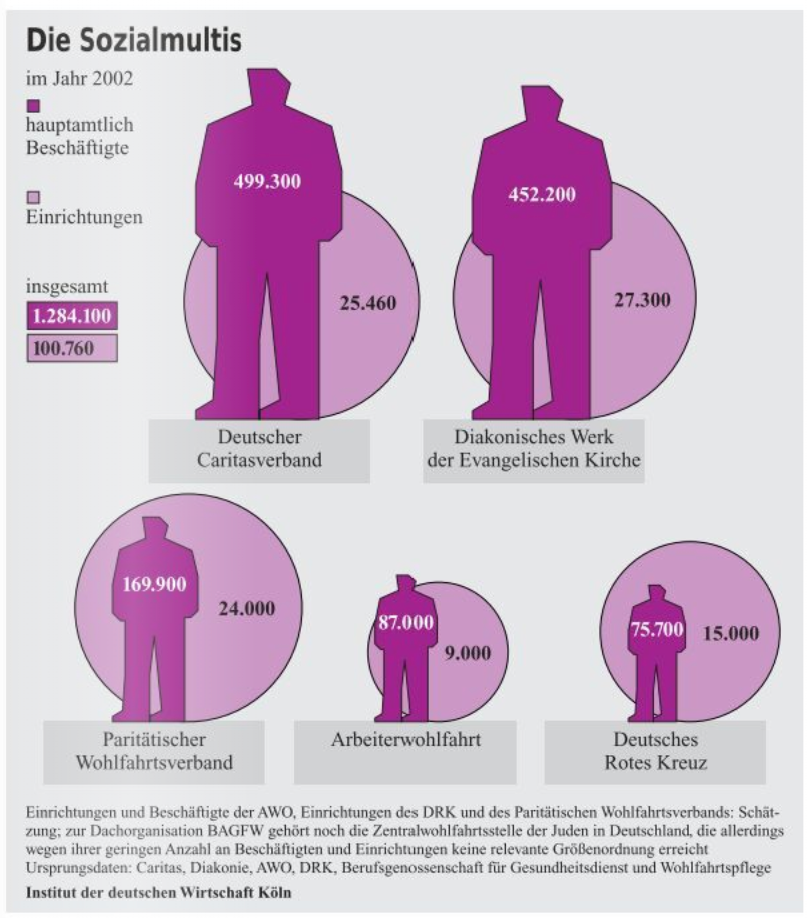
\includegraphics[keepaspectratio]{images/figure12.png}} \hfill{}

\caption{Abb. 1.2: Sozialunternehmen und Beschäftigte in der
Sozialwirtschaft (Institut der Deutschen Wirtschaft Köln 2004, S. 9,
\href{https://www.yumpu.com/de/document/view/7199735/auf-den-schultern-der-schwachen}{Link})}

\end{figure}%

Man kann deutlich erkennen, dass die konfessionellen Träger wie der
Caritasverband und auch das Diakonische Werk sowohl die meisten
Einrichtungen betreiben als auch die meisten Mitarbeitenden haben.
Darüber hinaus sind natürlich auch die anderen größeren
Wohlfahrtsverbände zu nennen, wie der Paritätische Verband, die
Arbeiterwohlfahrt und das Deutsche Rote Kreuz. Alle gemeinsam
beschäftigten im Jahre 2020 etwa rund 1,3 Millionen Menschen. Von den
Sozialmultis werden bundesweit ungefähr 100.000 Einrichtungen betrieben.
Wenn man die Träger der freien gemeinnützigen Wohlfahrtspflege
hinzunimmt, macht das ungefähr 5\% der gesamtwirtschaftlichen Leistung
aus. Wir haben ungefähr 43 Millionen Erwerbstätige in Deutschland (z. B.
Beck et al. 2013). In einem Gutachten zur Sozialwirtschaft in Sachsen
unter besonderer Berücksichtigung der Freien Wohlfahrtspflege vom
\href{https://tu-dresden.de/bu/wirtschaft/wwsprofecon/ressourcen/dateien/publikationen/Sozialwirtschaft_2011.pdf?lang=de}{Gesundheitsökonomischen
Zentrum an der TU Dresden} wurde berechnet, dass in Sachsen der Anteil
des Bereichs der „freigemeinnützigen Wohlfahrtspflege'' an der
Bruttowertschöpfung bei ungefähr 7,15\% liegt (Bundesdurchschnitt:
6,74\%) (Karmann et al. 2011).

Im Jahr 2008 gab es in Deutschland ca. 2,5 Millionen Mitarbeitende in
der Sozial- und Gesundheitswirtschaft (es wird hier der
Gesundheitsbereich hinzugerechnet) und auf europäischer Ebene rechnen
wir etwa mit 11 Millionen Mitarbeitenden in den genannten Bereichen
((Beck et al. 2013)). Wenn man dann die Wirtschaftsleistung in der
Europäischen Union betrachtet und den öffentlichen Sektor herausrechnet,
dann machen Unternehmen der Sozialwirtschaft ungefähr 10\% der
Bruttowertschöpfung aus, die eben nur der Sozialwirtschaft zugeordnet
werden können und das Gesundheitswesen ist hier in dem Fall nicht
mitgezählt (Beck et al. 2013).

\subsection{Beschäftigungszahlen}\label{beschaeftigungszahlen}

Gehen wir einmal noch auf eine andere Statistik ein, und zwar auf die
Beschäftigungszahlen in der Sozial- und Gesundheitswirtschaft. Hier sind
die Zahlen von 2014 und 2020 gegenübergestellt, die sich in den
jeweiligen Jahresberichten der Bundesagentur für Arbeit (Bundesagentur
für Arbeit Berichte 2014/2020) zum Juli des Jahres (saisonbereinigt)
finden. Im Bereich Erziehung und Unterricht sind im Jahr 2014 1.164.300
sozialversicherungspflichtig Beschäftigte angestellt gewesen. In 2020
waren bereits rund 1.347.000 Angestellte beschäftigt (15\%ige
Steigerung). In einem ähnlichen Umfang ist auch das
Beschäftigungswachstum im Bereich Gesundheitswesen auf 2.585.000
(+13,0\%) und im Bereich Heime und Sozialwesen auf 2.474.000 (+20,6\%)
gestiegen. Diese Zahlen bieten eine kurze Einordnung der
Sozialwirtschaft. Im Verhältnis dazu können wir von ungefähr 43
Millionen Erwerbstätigen in allen Branchen ausgehen.

\subsection{Finanzierungsmix für Träger der freien
Wohlfahrtspflege}\label{finanzierungsmix}

Wenn wir auf die Einnahmenseite blicken und die Frage stellen, wie denn
die freie Wohlfahrtspflege finanziert wird, dann wird deutlich, dass es
einen grundsätzlichen Mix aus unterschiedlichen Finanzierungsquellen
gibt (vgl. dazu \hyperref[figure13]{Abb. 1.3}).

\begin{figure}

\pandocbounded{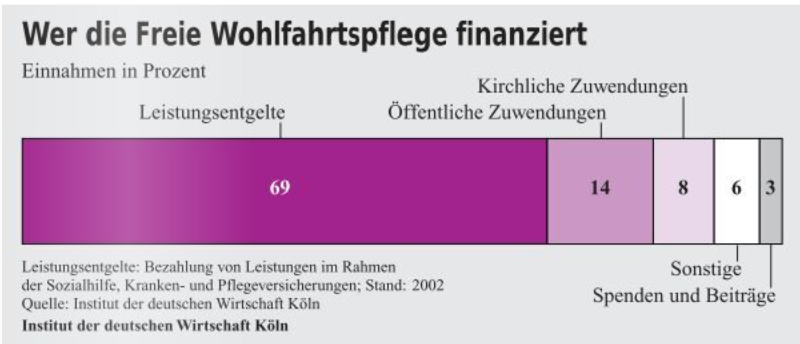
\includegraphics[keepaspectratio]{images/figure13.png}} \hfill{}

\caption{Abb. 1.3: Finanzierung der freien Wohlfahrtspflege (Institut
der Deutschen Wirtschaft Köln 2004, S. 29,
\href{https://www.yumpu.com/de/document/view/7199735/auf-den-schultern-der-schwachen}{Link})}

\end{figure}%

Nach einer Untersuchung des Instituts der deutschen Wirtschaft Köln
(Institut der Deutschen Wirtschaft Köln 2004) bestreiten zu 69\% freie
Träger ihr Einkommen aus den Leistungsentgelten. Leistungsentgelte sind
öffentliche Zuwendungen bzw. öffentliche Mittel, wie z. B. abgerechnete
Pauschalen, geleistete Fachleistungsstunden oder auch Tagessätze.
Darüber hinaus gibt es öffentliche Zuwendungen, z. B. im Rahmen von
Projekten oder institutionellen Finanzierungen. Die konfessionellen
Träger finanzieren sich teilweise noch aus kirchlichen Zuwendungen.
Schließlich gibt es noch eine Reihe von sonstigen Quellen, wie z. B.
Projektmittel, Spenden und Beiträge. Beiträge gibt es in gemeinnützigen
Einrichtungen und Organisationen, die Mitglieder haben, wie z. B.
Vereine oder Genossenschaften. Dazu zählen auch Elternbeiträge in der
Kita. Was man hier deutlich sieht -- und das ist gleichzeitig ein
Markenzeichen für die Sozialwirtschaft -- ist, dass wir es grundsätzlich
mit unterschiedlichen Finanzierungsquellen zu tun haben. Zum Erfolg
einer Einrichtung bzw. zu deren Gesamtfinanzierung reichen eben
öffentliche Mittel, die für die Finanzierung von Leistungen benötigt
werden, nicht zwingend aus. Vielmehr müssen wir uns Gedanken darüber
machen, wie wir den restlichen Betrag refinanzieren können, der nicht
auf öffentlichen, sondern dann aus privaten bzw. Eigenmitteln oder aus
Beiträgen und Spenden finanziert werden muss.

\section{Non-Profit-Organisationen}\label{npo-organisationen}

\subsection{Begriff Non-Profit-Organisationen}\label{begriffnpo}

Im Folgenden wird näher darauf eingegangen, was
Non-Profit-Organisationen ausmacht. Konkret handelt es sich dabei um
\textgreater{} „alle diejenigen Organisationen, die weder
erwerbswirtschaftliche Firmen noch öffentliche Behörden der
unmittelbaren Staats- und Kommunalverwaltung sind. NPO sind ferner jene
Organisationen, die einem gesellschaftlich als sinnvoll und notwendig
anerkannten Leistungsauftrag folgen und dabei nicht in erster Linie vom
Ziel der Gewinngenerierung geleitet werden. Nonprofit-Organisationen
werden dabei gemeinhin als Teil des sogenannten „Dritten Sektors''
verstanden, der neben bzw. zwischen den beiden idealtypischen ‚Polen'
Markt und Staat angesiedelt ist'' (Helmig 2019).

Demzufolge sind Non-Profit-Organisationen also solche Organisationen,
die nicht zum Staat und nicht zum Wirtschaftssektor gehören und
gewissermaßen den dritten Sektor in der Gesellschaft bilden. Sie
verfolgen keine Gewinnmaximierungsziele, sondern gehen einem
öffentlichen anerkannten bzw. gesetzlich geregelten Auftrag nach (siehe
\hyperref[table1]{Tab. 1}).

\begin{longtable}[]{@{}
  >{\raggedright\arraybackslash}p{(\linewidth - 2\tabcolsep) * \real{0.3913}}
  >{\raggedright\arraybackslash}p{(\linewidth - 2\tabcolsep) * \real{0.6087}}@{}}
\toprule\noalign{}
\begin{minipage}[b]{\linewidth}\raggedright
\textbf{Organisationsbereiche (nach Funktionen)}
\end{minipage} & \begin{minipage}[b]{\linewidth}\raggedright
\textbf{Typen von Organisationen}
\end{minipage} \\
\midrule\noalign{}
\endhead
\bottomrule\noalign{}
\endlastfoot
\textbf{Wirtschaftliche Organisationen} & Wirtschafts- und
Arbeitgeberverbände \\
& Gewerkschaften \\
& Berufsverbände \\
& Verbraucherorganisationen \\
\textbf{Soziokulturelle Organisationen} & Sportorganisationen \\
& Freizeitvereine \\
& Heimatvereine \\
& Diverse Kirchen, Sekten \\
& Organisationen in den Bereichen von Kunst und Kultur, von \\
& Wissenschaft und Forschung und von Bildung und Erziehung \\
& Organisationen zur Gestaltung der Lebenswelt (Wohnumfeld, \\
& Nachbarschaft etc.) \\
\textbf{Politische Organisationen} & Politische Parteien \\
& Natur- und Umweltorganisationen \\
& Politisch orientierte Organisationen \\
& Organisierte Bürgerinitiativen \\
\textbf{Karitative Organisationen} & Hilfsorganisationen für bestimmte
Bevölkerungskreise (Betagte, \\
& Behinderte, Kranke, Süchtige, Benachteiligte, Geschädigte); \\
& Wohlfahrtsverbände und deren Einrichtungen \\
& Entwicklungshilfeorganisationen \\
& Organisierte Selbsthilfegruppen mit karitativen Zwecken \\
\end{longtable}

Tab. 1: Typen privater Non-Profit-Organisationen
\phantomsection\label{table1}{Schwarz (1986), S. 7}

Auf die Frage, welche Arten von Non-Profit-Organisationen existieren,
gibt die folgende Abbildung einige Anhaltspunkte:

\begin{itemize}
\tightlist
\item
  \emph{Wirtschaftliche Organisationen}~wie z. B. Gewerkschaften,
  Arbeitgeberverbände und Verbraucherorganisationen;
\end{itemize}

\begin{itemize}
\item
  \emph{Soziokulturelle Organisationen}~wie z. B. Sportvereine,
  Organisation für Kunst und Kultur sowie wissenschaftliche
  Einrichtungen;
\item
  \emph{Politische Organisationen}~wie z. B. Parteien, Umweltbewegungen,
  Umweltverbände;
\item
  \emph{Karitative Organisationen}, die sich um die Hilfe für Menschen
  in besonderen Lebenslagen kümmern, wie z. B. Wohlfahrtsverbände und
  Entwicklungshilfeorganisationen.
\end{itemize}

Non-Profit-Organisation sind demzufolge alle Organisationen in der
Gesellschaft, die prinzipiell gemeinnützige Zwecke, aber darüber hinaus
auch wirtschaftliche Zwecke verfolgen können, aber nicht zwingend auf
eine Gewinnmaximierung aus sind. Wenn wir demgegenüber von der
Sozialwirtschaft reden, müssen wir noch eine Einschränkung vornehmen. Es
gibt zwar viele Organisationen, die hier in die Kategorie
Soziokulturelle Organisationen fallen, z. B. Organisationen zur
Förderung von Kultur oder Bildung und Erziehung. Hinzugezählt werden
müssen auch diejenigen Organisationen, die der Gestaltung des
Lebensumfeldes dienen, und auch karitative Organisationen, also alle
Wohlfahrtsverbände, Hilfsorganisationen und freigemeinnützige
Einrichtungen. Nichtsdestotrotz gibt es auch Graubereiche: Soziale
Organisationen, also spezifische Non-Profit-Organisationen; der Begriff
muss später noch näher bestimmt werden.

\subsection{Gemeinsamkeiten und Unterschiede zwischen Profit- und
Non-Profit-Organisationen}\label{vergleichnpo}

Zur genaueren Differenzierung von Non-Profit-Organisationen und
erwerbswirtschaftlichen Organisationen ist folgende
\hyperref[figure14]{Abb. 1.4} hilfreich (Schwarz 1986, S. 8).

\begin{figure}

\pandocbounded{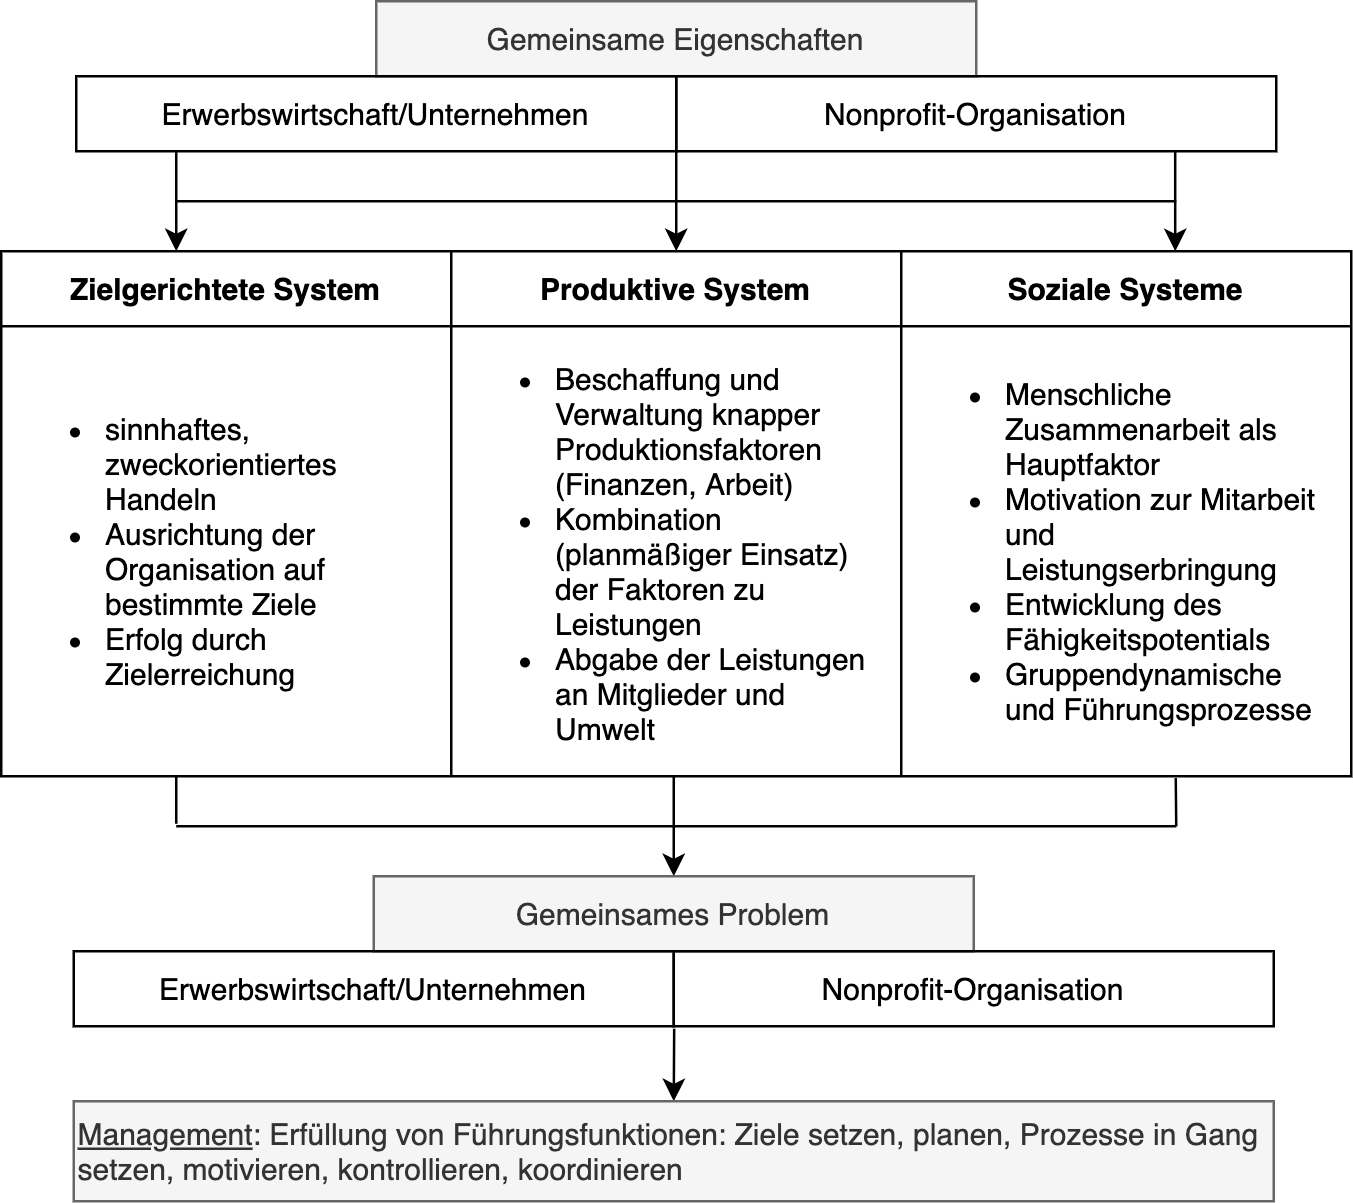
\includegraphics[keepaspectratio]{images/figure14.png}} \hfill{}

\caption{Abb. 1.4: Gemeinsamkeiten und Unterschiede zwischen NPO und
Unternehmen (nach Schwarz 1986, S. 8)}

\end{figure}%

\subsubsection{Gemeinsamkeiten}\label{npogemeinsamkeiten}

Nach Schwarz (1986) bestehen alle Organisationen, egal ob sie
erwerbswirtschaftliche (For-Profit) oder nicht-erwerbswirtschaftliche
(Non-Profit) Unternehmen darstellen, aus verschiedenen Teilsystemen.
Organisationen sind immer zugleich zielgerichtete Systeme, produktive
Systeme und soziale Systeme. Damit ist gemeint, dass jede Organisation
immer zu einem konkreten Zweck gegründet wurde, der -- wenn vorhanden --
in der Satzung bzw. im Gesellschaftervertrag der gegründeten Einrichtung
niedergeschrieben ist, und der die Grundlage bildet für das gesamte
Arbeiten in der Organisation. Darüber hinaus sind alle diese
Organisationen auch produktive Systeme, d.~h. hier geht es um die Frage,
wie ist der Personaleinsatz in der Einrichtung organisiert, welche
finanziellen Ressourcen stehen zur Verfügung, wie kann man neue
Finanzierungsquellen aufschließen und wie werden Produkte und
Dienstleistungen angeboten. Darüber hinaus sind alle Organisationen auch
soziale Systeme. Es gilt immer mit zu bedenken, wie Mitarbeitende
motiviert und dabei unterstützt werden können, ihre Kompetenzen
weiterzuentwickeln. Im Vordergrund des sozialen Systems steht also der
Faktor „Humankapital''

Alle Organisationen, sind sie denn einmal gegründet, müssen sich damit
auseinandersetzen, wie das Management ihrer Einrichtung zu funktionieren
hat, also welche Führungsprozesse zu organisieren sind, wie Ziele
gesetzt werden, wie geplant wird, wie etwa Personalplanung stattfindet
und wie Koordinierung und Organisationen im engeren Sinne in der
Einrichtung umgesetzt werden kann. All das sind Aufgaben, die jede
Einrichtung zu erfüllen hat. Kurz zusammengefasst: Auch
Non-Profit-Organisationen müssen sich mit dem Management, also mit
ökonomischen Fragestellungen auseinandersetzen und haben ähnliche
Rahmenbedingungen zu beachten wie auch erwerbswirtschaftliche
Organisationen bzw. umgekehrt.

\subsubsection{Unterschiede}\label{npounterschiede}

Und man kann neben den Gemeinsamkeiten auch verschiedene Unterschiede
herausarbeiten, auch das geht hier auf eine Untersuchung von Schwarz
Schwarz (1986) zurück (vgl. \hyperref[table2]{Tab. 2}).

\begin{longtable}[]{@{}
  >{\raggedright\arraybackslash}p{(\linewidth - 4\tabcolsep) * \real{0.2394}}
  >{\raggedright\arraybackslash}p{(\linewidth - 4\tabcolsep) * \real{0.3310}}
  >{\raggedright\arraybackslash}p{(\linewidth - 4\tabcolsep) * \real{0.4296}}@{}}
\toprule\noalign{}
\begin{minipage}[b]{\linewidth}\raggedright
\textbf{Strukturmerkmale}
\end{minipage} & \begin{minipage}[b]{\linewidth}\raggedright
\textbf{For-Profit Unternehmen}
\end{minipage} & \begin{minipage}[b]{\linewidth}\raggedright
\textbf{Non-Profit Organisationen}
\end{minipage} \\
\midrule\noalign{}
\endhead
\bottomrule\noalign{}
\endlastfoot
\textbf{Hauptzweck} & Erwirtschaftung eines möglichst hohen Ertrags auf
das investierte Kapital für Eigentümer (Formalziele: Gewinn und
Rentabilität) -- Erwerbswirtschaft & Erbringung von Leistungen für
bestimmten Personenkreis in der Sozial- und Gesundheitswirtschaft
(Sachziel: satzungsgemäße Zwecke) -- Bedarfswirtschaft \\
\textbf{Adressaten und Marktbeziehung} & Deckung des Fremdbedarfs von
Nachfrage durch Angebot auf Märkten & Deckung des Eigenbedarfs von
Mitgliedern, Klienten etc. und des gesellschaftlichen Bedarfs
(Identitätsprinzip: Mitglied = Kunde) \\
\textbf{Steuerungsprinzipien} & Marktorientierung, Ausrichtung an
Kunden- und Wettbewerberverhalten & Marktsteuerung teils nicht existent,
teils sekundär; Mitglieder bestimmen demokratisch (direkt) oder durch
indirektes Verhalten über Leistung (Versorgungs- und
Bedarfsorientierung) \\
\textbf{Güter und Dienstleistungen} & Nur private marktfähige
Individualgüter, die ausschließlich vom einzelnen Käufer genutzt werden
können & Kollektivgüter, die einer ganzen Gruppe zugutekommen, auch
denjenigen, die nicht dafür zahlen können; hauptsächlich
Dienstleistungen \\
\textbf{Finanzmittel} & Kapitalanlagen und Umsatzerlöse &
Mitgliedsbeiträge, Leistungsentgelte, Spenden, Steuervergünstigungen
etc. \\
\end{longtable}

Tab. 2: Unterscheidung von Unternehmen der Erwerbswirtschaft und
Non-Profit-Organisationen \phantomsection\label{table2}{Schwarz (1986)}

Der Hauptzweck von Non-Profit-Organisationen ist insbesondere, dass hier
Leistungen für einen ganz bestimmten Personenkreis der Sozial- und
Gesundheitswirtschaft erbracht werden. Man spricht in diesem
Zusammenhang auch von einer Bedarfswirtschaft, d.~h. es wird immer
anhand von gesetzlichen Rahmenbedingungen bzw. den Bedürfnissen der
jeweiligen Zielgruppe aus geplant, während die Erwerbswirtschaft stärker
den Blick darauf richtet, das eingesetzte Kapital und den Ertrag zu
steigern. In der Erwerbswirtschaft steht daher der Gewinn und die
Rentabilität im Blick als Formalziele im Vordergrund. Profitorientierte
Organisationen haben die Nachfrage und das Angebot auf Märkten im Blick,
während Non-Profit-Organisationen den Eigenbedarf ihrer Mitglieder,
Klient*innen bzw. allgemein den gesellschaftlichen Bedarf
berücksichtigen müssen. Man spricht in letzterem Fall von sozialen
Märkten bzw. vom Gesundheitsmarkt, was einen abgegrenzten Bereich
darstellt.

Ebenso unterscheiden sich die Steuerungsprinzipien zwischen Profit- und
Non-Profit-Bereich. Die Erwerbswirtschaft orientiert sich am Markt und
richtet ihre Produkte und Dienstleistungen an den möglichen
Entwicklungen im Markt aus. Dabei müssen Wettbewerb, Kundenorientierung
und das Verhalten der Wettbewerber und Kunden ständig analysiert werden,
während es bei den Non-Profit-Organisationen eher darum geht, dass
Mitglieder mitbestimmen können, wie die Einrichtungen sich entwickeln
und auch, dass insbesondere die Perspektiven der Klient*innen in den
Mittelpunkt geschoben werden. Die angebotenen Güter und Dienstleistungen
unterscheiden sich zwischen Profit- und Non-Profit-Organisationen.
Profitorientierte Organisationen setzen die auf Märkten gehandelte
Individualgüter ab. Es kann natürlich auch Produktionsgüter geben.
Schwarz (1986) sagt, dass Non-Profit-Organisationen tendenziell eher
Kollektivgüter produzieren, mit anderen Worten also soziale
Dienstleistungen anbieten. Auch hinsichtlich der Finanzmittel gibt es
Unterschiede. Profitorientierte Organisation können beispielsweise Geld
am Kapitalmarkt anlegen und finanzieren sich aus Umsatzerlösen. Bei den
Non-Profit-Organisationen existieren verschiedene Einnahmequellen, wie
z. B. Leistungsentgelte, öffentliche Zuwendungen, Mitgliederbeiträge
oder Spenden.\\
\strut \\
Abschließend muss der hier nach Schwarz (1986) vorgestellte Ansatz noch
einmal kritisch betrachtet werden. Diese Übersicht ist natürlich eine
Vereinfachung, um wesentliche Unterschiede zwischen diesen Typen von
Unternehmen herauszuarbeiten. Die Übersicht stammt auch aus den 1980er
Jahren und wurde in verschiedenen Lehrbüchern immer wieder reproduziert.
Daher nehmen wir hier auch Bezug darauf. Beachtet werden muss
allerdings, dass sich die Grenzen zwischen Profit- und
Non-Profit-Organisationen über die letzten Jahre hinweg verschoben
haben. Selbstverständlich gibt es auch Grenzbereiche bzw. eine Grauzone.
So gibt es natürlich auch viele Non-Profit-Organisationen, die neben
ihrer gemeinnützigen Arbeit auch noch einen wirtschaftlichen
Geschäftsbetrieb besitzen und dort eine Gewinnmaximierung verfolgen
können. Genauso gibt es auch For-Profit-Organisationen, die im Bereich
der Sozialwirtschaft tätig sind, wie z. B. Pflegeeinrichtungen für
einkommensstärkere Bevölkerungsgruppen, die durch Eigen- bzw.
Selbstbeiträge andere und umfangreichere Dienstleistungen (über den
gesetzlichen Anspruch hinaus) beanspruchen können. All das sind
sozusagen auch erwerbswirtschaftliche Sichtweisen bzw. Elemente, die
auch in der Sozialwirtschaft immer mehr an Bedeutung gewinnen. Das
bringt uns zu dem Punkt, dass wir bei der Unterscheidung von For-Profit-
und Non-Profit-Organisationen von einem breiten Spektrum ausgehen
müssen. Auf der anderen Seite des Spektrums stehen idealtypisch die
For-Profit-Organisationen, auf der anderen Seite die
Non-Profit-Organisationen. In der Realität befinden wir uns
möglicherweise immer zwischen diesen verschiedenen Idealtypen. Im
Folgenden werden wir demnach Organisationen in den Blick nehmen, die
„tendenziell'' Non-Profit-Organisationen darstellen und die im erwähnten
Spannungsfeld zwischen diesen beiden Polen stehen.

\section{Begriff Soziale
Organisation}\label{begriff-soziale-organisation}

In Abgrenzung zum Begriff Non-Profit-Organisation wird nunmehr noch eine
Abgrenzung zu dem der „Sozialen Organisation'' notwendig. Die Merkmale
von Sozialen Organisationen lassen sich wie in der folgenden Liste
versuchen festzumachen:

\begin{itemize}
\item
  Soziale Einrichtungen sind insbesondere Unternehmen, die
  Sozialdienstleistungen erbringen und/oder Güter und Dienstleistungen
  für besonders schutzbedürftige Bevölkerungsgruppen und entsprechend
  gesetzlicher Aufträge (z. B. Erziehung, Betreuung, Lernen) anbieten.
  Diese Sozialunternehmen streben im Rahmen der Produktion von Waren
  bzw. bei der Erbringung von Dienstleistungen ein soziales Ziel an.
\item
  Sie zielen im Sinne der Gemeinnützigkeit auf eine Bedarfs- und
  Kostendeckung anstatt auf Gewinnmaximierung. Nichtsdestotrotz müssen
  auch soziale Einrichtungen Gewinne erwirtschaften, d.~h. am Ende des
  Jahres muss etwas überbleiben. Dieser Überschuss muss allerdings
  wieder dem Einrichtungszweck zugutekommen. Die Gemeinnützigkeit ist in
  der Abgabenordnung geregelt, nach der der Gesetzgeber den als
  gemeinnützig anerkannten Einrichtungen Steuerermäßigungen/-befreiungen
  einräumt, wie z. B. für Ertragsteuern, Umsatzsteuer etc.
\item
  Sie offerieren „soziale personenbezogene Dienstleistungen'' (Klatetzki
  2010), die sich aus gesetzlich normierten Aufträgen (z. B.
  \href{https://www.bpb.de/kurz-knapp/lexika/politiklexikon/18231/sozialgesetzbuch-sgb/}{SGB})
  ergeben. Eine Besonderheit dieser Art von Dienstleistungen ist es,
  dass diese in dem Moment, wenn sie angeboten werden, bereits
  verbraucht werden, weil hier Produktion und Konsumption gewissermaßen
  zusammenfallen. Soziale personenbezogene Dienstleistungen können nur
  schwer standardisiert werden. Anders als bei einem Werkstück, was man
  in eine Maschine einspannt und ausmessen kann, sind hier
  professionelle Normen, Haltungen und Ansprüche gemeint, die wie
  Dienstleistung angeboten werden.
\item
  Schließlich sind soziale Organisationen dadurch gekennzeichnet, dass
  sie Ehrenamtliche und Freiwillige in die Erfüllung ihrer verschiedenen
  Sachziele einsetzen, was in erwerbsorientierten Organisationen in der
  Regel nicht der Fall ist.
\end{itemize}

\section{Herausforderungen in der
Sozialwirtschaft}\label{herausforderungen-sozialwirtschaft}

\subsection{Ausgangspunkt}\label{sozialwirtschaft-ausgangspunkt}

Träger und Einrichtungen in der Sozialwirtschaft müssen stärker
ökonomische Fragen beachten und sich auch am marktwirtschaftlichen
Wettbewerb ausrichten.

Es gibt eine Betätigung auf sozialen Märkten, darüber hinaus ist ein
weiteres, immer noch sehr spezielles Kennzeichen für den Bereich der
Sozialwirtschaft aber auch die Finanzierung. In der Sozialwirtschaft
haben wir es mit einer Vielzahl von Monopolanbietern zu tun. Aus
sozialrechtlicher Perspektive werden diese auch als Leistungsträger
bezeichnet, die gewissermaßen die Leistungen refinanzieren und auch die
notwendigen finanziellen Mittel zur Verfügung stellen. Es ist aber immer
eine Bewerbung notwendig oder die Leistungen müssen beantragt werden --
gegebenenfalls muss auch eine Leistungsvergütung berechnet und
vertraglich geregelt werden (meistens durch Entgeltverträge).
Sozialunternehmen sind daher in hohem Maß abhängig von den
Leistungsträgern und man kann hier größtenteils von einem Monopolmarkt
sprechen.

Als Konsequenz ergibt sich die Notwendigkeit, sich stärker mit
Managementkompetenzen auseinanderzusetzen. In Ihrer Ausbildung lernen
Sie genau deswegen auch verschiedene Grundlagen des Managements, weil
diese notwendig sind, um zukünftig in der Einrichtungsleitung zu
arbeiten bzw. um einen guten Job zu verrichten. Wirtschaftliche
Grundkenntnisse gehören genauso zum Berufsbild wie die
sozialpädagogische Professionalität.

\subsection{Hybrid-Funktionen des Sozialmanagements und des Managements
in der Sozialwirtschaft}\label{sozialwirtschat-hybriditaet}

Es gilt immer, einen Fokus auf die Ressourcen zu legen, d.~h. es ist
stets auf einen effektiven und effizienten Einsatz von Ressourcen zu
achten. Fragen der Finanzierung, der Investitionsrechnung, des
Controllings und verschiedener anderer Aspekte dieser Hard Facts müssen
berücksichtigt werden.

Um Einrichtungen der Sozialwirtschaft überhaupt betreiben zu können,
gilt es, sich mit der Akquise unterschiedlicher Finanzierungsquellen zu
beschäftigen. Insbesondere in der Sozialwirtschaft existieren
unterschiedliche Finanzierungsquellen und auch verschiedene Quellen
jenseits der öffentlichen Mittel, privaten Mittel oder Spenden. Solche
Einnahmen müssen erst einmal akquiriert werden und zudem gilt es,
gleichzeitig noch den Blick zu öffnen für die Mitarbeiter*innen der
Einrichtung, die unter enormen Stress und enormen Belastungen ihre
Dienste erbringen. Darüber hinaus muss auch auf die Personalentwicklung
geachtet werden. Den Mitarbeiter*innen müssen Möglichkeiten für
Weiterbildung und für Karriereentwicklung geboten werden. All das sind
die besonderen Kennzeichen und Herausforderungen in der
Sozialwirtschaft.

Die Sozialwirtschaft ist durch Hybridität gekennzeichnet. Das bringt
besondere Herausforderungen in der Umsetzung des Managements sozialer
Einrichtungen mit sich. Damit ist gemeint -- und hier sei auf die Grafik
von Armin Wöhrle (2007) in dem Buch von Volker Brinkmann (2010)
hingewiesen --, dass das Sozialmanagement hier in die Mitte des
Aktionsfeldes gestellt werden kann und man überlegen sollte, welche
anderen Bereiche noch zu beachten sind (vgl. \hyperref[figure15]{Abb.
1.5}).

\begin{figure}

\pandocbounded{\includegraphics[keepaspectratio]{images/figure15.png}} \hfill{}

\caption{Abb. 1.5: Hybrid‐Funktionen des Sozialmanagements nach Arnold
(2022a) in Anlehnung an Armin Wöhrle (2007) zit. n. Brinkmann (2010, S.
25)}

\end{figure}%

Wenn man den äußeren Kreis in der \hyperref[figure15]{Abb. 1.5}
betrachtet, lassen sich eine Reihe von Fachdisziplinen ausfindig machen,
die im Sozialmanagement eine Rolle spielen: u. a. Volkswirtschaftslehre,
Betriebswirtschaftslehre, Public Management. In diesen Disziplinen
stellt man sich die Frage, was denn an Wirtschaftlichkeitserwägungen in
der Gestaltung von sozialen Organisationen beachtet werden soll. Darüber
hinaus müssen auch soziale, politische, rechtliche und
verwaltungsbezogene Grundlagen beachtet werden. Zusätzlich braucht es
fundiertes Wissen aus den Sozialwissenschaften: Es braucht
sozialwissenschaftliche Grundlagen wie z. B. aus der Arbeits- und
Organisationspsychologie, um zu verstehen, wie Personalentwicklung,
Personalführung, Organisationsentwicklung und dergleichen gestaltet
werden können.

Natürlich hat die Disziplin der Sozialen Arbeit darüber hinaus eine
maßgebliche Bedeutung für die Fragestellung: Wie können wir auf der
einen Seite die Professionalität und das Qualitätsverständnis der
Sozialen Arbeit und auf der anderen Seite die ökonomischen
Rahmenbedingungen zusammenführen, sodass sich dies nicht gegenseitig
ausschließt, sondern wie zwei Zahnräder, die ineinandergreifen,
zusammengeführt werden?

Die Herausforderung, die sich für die Sozialwirtschaft, also für
Sozialunternehmen ergeben, sind mindestens zweiteilig. Auf der einen
Seite kann man von Multirationalität, auf der anderen Seite von Hybrid
sprechen. Was ist mit diesen Konzepten gemeint? Darauf soll im Folgenden
näher eingegangen werden.

\subsection{Multirationalität und
Hybridität}\label{multirationalitt-und-hybriditaet}

\subsubsection{Multirationalität}\label{sozialwirtschat-multirationalitaet}

Multirationalität\footnote{Ein Einführungsvideo gibt es an dieser
  Stelle: \url{https://www.youtube.com/watch?v=L_Mf-tNNFJc}} ist ein
Begriff, der insbesondere vom Autorenteam Schedler and Rüegg-Stürm
(2013) geprägt wurde, die sich mit der Frage auseinandergesetzt haben,
wie die verschiedenen Rationalitäten, mit anderen Worten die
verschiedenen Ansprüche, Zielstellungen, Wünsche sowie Interessen, die
innerhalb und außerhalb einer Organisation existieren, zusammengebracht
werden können. Sie meinen, dass dauerhaft und zeitgleich immer mehrere
dieser Rationalitäten und Logiken existieren und es dabei durchaus auch
zu Widersprüchen kommen kann in einer Organisation. All das gilt es zu
„managen'', in den Blick zu nehmen und sozusagen als Motivation für die
Zusammenarbeit aufzufassen.

Zum Beispiel gibt es verschiedene Fachsprachen in der Einrichtung, d.~h.
bei professionellem Zusammenarbeiten gibt es unterschiedliche
Stakeholder-Interessen. Dies sind die Interessen der Mitarbeitenden, die
Sie vertreten, die der Leitung und auch die der Klient*innen.

Es sind noch Rahmenbedingungen der Politik und Ökonomie zu beachten. All
das sind unterschiedliche Perspektiven, die immer gleichzeitig
betrachtet werden müssen, wenn es um die Aufgabenkoordination und die
Lösung von Problemen im Arbeitsalltag geht.

\subsubsection{Hybridität}\label{sozialwirtschat-hybriditaet}

Neben der Multirationalität gibt es noch ein anderes Prinzip, nämlich
das der Hybridität. Dieses geht stärker auf die Autoren Evers and Ewert
(2010) zurück. Der Begriff Hybridität kommt aus den Kulturwissenschaften
und meint, dass Dinge, die miteinander zusammengeführt werden,
ineinanderfließen und dass es zu Überschneidungen kommt. Im Kontext der
Sozialwirtschaft geht es dabei um den Einfluss unterschiedlicher,
wechselseitig bedingender Werte und Logiken, die aber nicht nur
innerhalb einer Organisation existieren, sondern auch zwischen den
verschiedenen Sektoren der Gesellschaft vorliegen können. Mit Sektoren
der Gesellschaft ist gemeint, dass es einerseits soziale Leistungen im
sozialen Markt gibt und gleichzeitig auch der öffentliche Bereich
mitgedacht werden muss. Also der Kostenträger bzw. die öffentlichen
Einrichtungen, die die angebotenen personenbezogenen sozialen
Dienstleistungen finanzieren, sind einzubeziehen. Darüber hinaus kann es
auch noch andere gesellschaftliche Interessen geben, nämlich wie die
Leistungen angeboten werden und wer die Bedürftigen bzw.
Anspruchsgruppen sind. Es sind darüber hinaus auch die rechtlichen
Rahmenbedingungen zu beachten, der Bereich der Jurisprudenz, und so
könnte man diese Beispiele noch ewig weiterführen.

Was hier zu beachten ist, ist, dass mit Hybridität nicht die des
(internen) Organisationsgeschehens betrachtet wird. Vielmehr werden
unter diesem Konzept die verschiedenen Sektoren der Gesellschaft -- also
die Organisationsumwelt -- in den Blick genommen. Ein Beispiel stellt
hier die Gemeinwesenarbeit dar. Diese kann man als eine „Bearbeitung''
und Gestaltung von Hybridität ansehen, weil das Zusammenarbeiten
verschiedenster Organisationen, Personen und Gruppen im Vordergrund
steht, ob dies nun die Stadt, ein freier Träger oder ein Kommunalverband
ist. Hier muss, um ein soziales Problem möglichst von unterschiedlichen
Perspektiven anzugehen, die Hybridität beachtet werden, also die
Zusammenarbeit von unterschiedlichen Sektoren der Gesellschaft
organisiert werden.

\subsubsection{Konsequenzen}\label{sozialwirtschat-konsequenzen}

Einerseits sind Ressourcen von Sozialunternehmen aus unterschiedlichen
Quellen zu nutzen, was oben unter dem Stichpunkt Finanzierungsmix
bereits ausgeführt wurde. Zweitens müssen verschiedene
Interessensgruppen miteinander ausgehandelt werden. Im Sinne des
Partizipationsprinzips und der Beteiligung von unterschiedlichen
Interessensgruppen ist es hilfreich, hier auch Selbstvertretungen in
Organisationen zu organisieren.

Darüber hinaus muss man die Formalziele mit den Sachzielen abwägen, d.
h. auf der einen Seite gibt es natürlich eine Gewinnerzielungsabsicht
und am Ende des Jahres muss mindestens plus/minus null erreicht werden.
Gleichzeitig muss aber auch der ideelle Auftrag, die Vision und der
Unternehmenszweck umgesetzt und erreicht werden (z. B. Betreuungs-,
Beratungs- und Bildungsleistungen).

Damit ist gemeint, dass Organisationen nach innen und nach außen
vertreten werden müssen und sich eine Organisationsidentität entwickelt:
Wofür stehen wir? Was ist unser Auftrag? Wer ist unsere Zielgruppe? All
diese Fragen müssen im Leitbild geklärt werden. Damit beschäftigen wir
uns noch einmal ausführlicher an späterer Stelle. Beide Konzepte, die
Multirationalität und die Hybridität, gewinnen in der Praxis zunehmend
an Bedeutung, insbesondere in der Abgrenzung zwischen Einrichtungen und
in der Gestaltung der Arbeitsbedingungen selbst.

\chapter{Funktionsbereiche}\label{funktionsbereiche}

Was die betriebswirtschaftlichen Funktionsbereiche in einem Unternehmen
sind, kann durch folgende Metapher eines Hauses erklärt werden: In dem
Haus, dem Haus der BWL, gibt es verschiedene Aufgaben- und
Funktionsbereiche, die es in einem Unternehmen generell zu organisieren
gilt. Dabei handelt es sich z.B. um die einzelnen Abteilungen bzw.
einzelnen Aufgabenbereiche, in denen sich jede Einrichtung aufgliedert,
unabhängig davon, ob Sie für Leitung- oder für fachliche Teilaufgaben in
einer Einrichtung zuständig sind. Mit anderen Worten sind das die
\emph{allgemeinen betriebswirtschaftlichen Aufgabenstellungen}, die auch
in jeder Sozialeinrichtung vorhanden sein müssen (vgl.
\hyperref[figure21]{Abb. 2.1}).

\begin{figure}

\pandocbounded{\includegraphics[keepaspectratio]{images/figure21.png}} \hfill{}

\caption{Abb. 2.1: Haus der BWL (eigene Darstellung)}

\end{figure}%

Das Fundament bilden die sozialen betriebswirtschaftlichen Grundlagen.
Hierauf wurde bereits weiter oben eingegangen und die Grundzusammenhänge
wurden schon erarbeitet.

In der Mitte des Hauses steht die rote Säule, einerseits
das~\emph{interne und externe Rechnungswesen}~und andererseits
das~\emph{Controlling}. Diese Bereiche stellen die Hard Facts und damit
gewissermaßen die zahlenmäßige Informationsbasis für wirtschaftliche
Zusammenhänge innerhalb der Einrichtung dar.
Die~\emph{Finanzierung}~wiederum ergänzt das Ganze, um eine Übersicht zu
den zur Verfügung stehenden finanziellen Mitteln, die eventuell
beschafft oder hinsichtlich ihrer Verwendung geprüft werden müssen, zu
bieten.

Dann gibt es die~\emph{Organisationstheorie und
Organisationsentwicklung}~zu betrachten. Das ist derjenige Teil, der
sich mit den organisations- und arbeitswissenschaftlichen Zusammenhängen
beschäftigt. Dabei geht es um die Frage, wer welche Aufgabe innerhalb
einer Einrichtung hat, wie sie strukturiert werden kann und wie Prozesse
verändert werden können.

Das~\emph{Personalmanagement}~beschäftigt sich mit der Frage, wie
Personen innerhalb von Einrichtungen geleitet, motiviert und geführt
werden und sich weiterentwickeln können.

Zurück zur Metapher: Das Haus hat noch Balkons: auf der linken Seite ist
das~\emph{Sozialmarketing}~zu finden. Das Sozialmarketing ist ein
spezifisches Marketing, was sich mit sozialen Einrichtungen beschäftigt.
Dabei kommen die allgemeinen Grundlagen aus der
Betriebswirtschaftslehre, die sich mit dem Marketing von Unternehmen
beschäftigen, zur Anwendung. Die allgemeinen Marketinggrundlagen müssen
aber übertragen und ggf. modifiziert werden, um sie in sozialen
Einrichtungen auch nutzen zu können.

Dann gibt es das~\emph{Qualitätsmanagement}. Dieses hat das Ziel, die
Professionalität und Qualität der Ziele und Ergebnisse sowie Strukturen
und Prozesse zu überprüfen. Des Weiteren gibt es
das~\emph{Projektmanagement}~und auch das~\emph{Change-Management}. Hier
geht es um die Frage der sinnvollen Durchführung von Projekten, deren
Planung und Umsetzung sowie deren Evaluierung und um die erfolgreiche
Organisationsentwicklung.

Schließlich gibt es noch den Bereich der~\emph{Evaluation und
Wirkungsmessung}. Das ist der Bereich, der sich mit der Wirkung von
Leistungen beschäftigt. Nicht nur im finanziellen Sinne, sondern ganz im
Gegenteil wird die Frage gestellt, welcher Beitrag geleistet wird, damit
die Qualität, also die Lebensqualität der Klient*innen verbessert wird.
Gleichzeitig stellt sich auch die Frage, wie möglicherweise Einfluss
darauf genommen werden kann, dass es in dem jeweiligen Stadtteil oder
der Region zu einer Verbesserung kommt. Wirkungsmessung in diesem
Zusammenhang bezieht sich auf die sozialen Wirkungen. Dies sind nicht
zwingend monetäre, sondern gerade auch die gesellschaftlichen
Veränderungen, die erzielt wurden: entweder durch die Tätigkeit der
Sozialarbeitenden oder durch sozialpädagogische Maßnahmen selbst.

Das Dach des Hauses könnte eigentlich auch der Keller sein: Hier
verbirgt sich das Aufgabenfeld~\emph{Existenzgründung und
Selbstständigkeit}. Es ist deswegen auf das Dach gesetzt worden, weil
hier alle Grundlagen, die vorher genannt wurden, zum Zuge kommen: Wenn
eine Einrichtung gegründet und dann die Finanzplanung gemacht werden
soll, braucht es die Finanzierung und das Rechnungswesen. Gleichzeitig
bedarf es auch der Kenntnisse des Personalwesens, Wissen über die
Strukturierung der Organisation und von einschlägigen rechtlichen
Rahmenbedingungen. Die anderen Maßnahmen, wie zum Beispiel das
Marketing, sind erforderlich, um überhaupt die Zielgruppe näher zu
bestimmen, den Markt einzuschätzen und auch die Wettbewerber
kennenzulernen. Das verstehen wir unter dem Haus der BWL.

\section{Rechnungswesen}\label{rechnungswesen}

\subsection{Überblick zum
Rechnungswesen}\label{ueberblick-zum-rechnungswesen}

Das Rechnungswesen wird auch als betriebliches Rechnungswesen bezeichnet
und hat die Aufgabe, die wirtschaftlichen Zusammenhänge in der
Einrichtung darzustellen. Hierbei sind vier Teile dieses Rechnungswesens
zu erörtern. Es gibt zwar noch weitere Teile, aber es soll hier erstmal
des Überblicks Willen um diese vier Teile gehen (vgl. im Folgenden
Arnold 2024).

\textbf{1. Teil: Finanzierung}

Die Finanzierung bzw. das Finanzmanagement ist eine zukunftsbezogene
Aufgabe mit dem Ziel, alle in der Einrichtung verfügbaren bzw. zu
akquirierenden Mittel zu verwalten bzw. die Zahlungsströme zu steuern.
Dadurch muss sich sodann die Zahlungsfähigkeit bestimmen lassen. Sie
lässt sich zum Beispiel mithilfe einer Liquiditätsplanung ermitteln.
Dabei werden die Einzahlungen den Auszahlungen gegenübergstellt und so
lässt sich relativ schnell erfassen, ob zusätzliche Finanzierungsmittel
notwendig sind oder ob schon mit den erwarteten Einzahlungen alle
Rechnungen beglichen werden können. Investitionsrechnung beschäftigen
sich mit der Frage, inwieweit sich Investitionen rentieren.

Wenn bspw. ein Gebäude und ein Grundstück erworben und gebaut werden
soll, dann müssen entsprechende finanzielle Mittel dafür aufgenommen
werden, z. B. durch einen Kredit. Die Frage, die sich sodann stellt,
ist, ab wann sich die eingesetzten Mittel tatsächlich rentiert haben,
also ab wann wieder positive Zahlen geschrieben werden. Bei der
Finanzierung geht es allgemein darum, wo bestimmte Mittel herkommen,
nämlich aus der Innenfinanzierung, der Außenfinanzierung, der Eigen-
oder Fremdfinanzierung. Hierbei wird danach unterschieden, ob eigene
Mittel (bspw. Einlagen von Gesellschaftern/durch Gewinnrücklagen) oder
ob Fremdmittel (bspw. Aufnahme eines Darlehens bei einer Bank)
eingesetzt werden.

\textbf{2. Teil: Finanzbuchhaltung}

Die Finanzbuchhaltung ist zeitraumbezogen und vergangenheitsorientiert,
womit gemeint ist, dass alles systematisch aufbereitet ist. Alle
Geschäftsvorfälle während eines Geschäftsjahres sind zu dokumentieren
und werden in Vorbereitung auf einen Jahresabschluss am Ende des Jahres
erledigt. Zum Inhalt des Jahresabschlusses: Es muss eine Bilanz
aufgestellt werden, welche die Gegenüberstellung von Vermögen und
Kapital darstellt. Darüber hinaus kann es noch andere Bestandteile
geben, wie z. B. die Gewinn- und Verlustrechnung. Hier werden die
Erträge und die Aufwendungen gegenübergstellt und somit gewissermaßen
der Erfolg am Ende des Jahres ermittelt: ein Gewinn oder Verlust.

\textbf{3. Teil: Kosten- und Leistungsrechnung}

Zur Abgrenzung: Die Finanzbuchhaltung wird auch als externes
Rechnungswesen bezeichnet, die Kosten- und Leistungsrechnung als
internes Rechnungswesen. Was ist der Unterschied? Die Finanzbuchhaltung
muss gesetzlichen Auflagen folgen: dem Handels- und Steuerrecht. Danach
müssen entsprechend auch die Bilanz und die Gewinn- und
Verlustrechnungen erstellt werden. Bei der Kosten- und Leistungsrechnung
haben wir diese rechtlichen Verpflichtungen im Regelfall nicht; es gibt
Ausnahmen wie z. B. für Pflegeeinrichtungen und Krankenhäuser. Im
internen Rechnungswesen, welches gegenwarts- und zukunftsbezogen ist,
müssen die tatsächlich angefallenen Kosten und Leistungen erfasst
werden. Dies sind die im jeweiligen Unternehmen entstandenen Kosten und
Leistungen. Diese sind in Einzel- und Gemeinkosten zu unterscheiden:
Einzelkosten lassen sich direkt zu den jeweiligen Kostenträgern
zuordnen, Gemeinkosten nur indirekt. Es handelt sich dabei um allgemeine
Kosten wie z. B. Verwaltungskosten. Die Ermittlung der Selbstkosten --
das ist das übergeordnete Ziel -- geben Auskunft darüber, welche
Gesamtkosten in einer Einrichtung entstanden sind.

\textbf{4. Teil: Controlling und Planungswesen}

Dieser Bereich stellt ebenso wie das interne Rechnungswesen eine
gegenwarts- bzw. zukunftsbezogene Aufgabe dar. Hier geht es darum,
Planabweichungen möglichst rechtzeitig und früh zu identifizieren.
Hierzu werden insbesondere Budgets verwendet, um festzustellen, ob
zwischen den tatsächlich angefallenen und den geplanten Kosten eine
Abweichung vorliegt. Die Budgetierung und die anderen Instrumente dienen
letztlich dazu, eine Wirtschaftlichkeitsüberprüfung zu ermöglichen sowie
die Kosten und Gewinne innerhalb der Einrichtung zu steuern. Budgets
sind häufig mehrstufig und beinhalten Kostenstellen für die einzelnen
Teile der Einrichtung. Das Controlling dient also allgemein der
Steuerung des Unternehmens. Kurzum: das Controlling und Planungswesen
ist gewissermaßen die praktische Umsetzung der verschiedenen Zahlen, die
im Rahmen der Kosten- und Leistungsrechnung, Finanzbuchhaltung und im
Finanzmanagement ermittelt worden sind.

\subsection{Die Finanzströme eines
Unternehmens}\label{die-finanzstrme-eines-unternehmens}

Bei der Betrachtung der Finanzströme eines Unternehmens ergibt sich
meist ein komplexes Bild, wie in der folgenden Abbildung dargestellt.
Dabei steht das Unternehmen in der Mitte und es gibt verschiedene
Stakeholder, die am Unternehmen beteiligt sind oder mit diesem in
verschiedenen finanziellen Beziehungen stehen, wie z. B. die
Gesellschafter der Einrichtung, die Finanzmärkte, die Absatzmärkte und
den Staat.

Die~\emph{Gesellschafter}~haben bei Gründung der Einrichtung eine
Einlage geleistet und haben sich dadurch an der Gründung finanziell
beteiligt. Sie haben einen Anspruch darauf, dass sie an den Gewinnen
bzw. Dividenden und Einnahmen beteiligt werden. Wenn sie ihre Einlage
zurückrufen wollen, haben sie ggf. auch einen Anspruch darauf, das
Kapital zurückerstattet zu bekommen.

An den Finanzmärkten kann eine~\emph{Fremdfinanzierung}~zum Beispiel
durch Kredite und durch Darlehen aufgenommen werden. Dafür haben die
Banken oder Kreditinstitute dann ein Anspruch darauf, mindestens die
Tilgung zurückzuerhalten. Dies kann schrittweise oder auch als Ganzes
geschehen und zusätzlich haben sie noch Zinsen vereinbart, die zu zahlen
sind.

Demgegenüber können auch~\emph{Geldanlagen am Finanzmarkt}gemacht
werden, z. B. auf einem Geldmarkt- oder ein Sparkonto. Dafür können
dann, wenn die finanzielle Lage und die Märkte es hergeben, entsprechend
Guthabenzinsen erwirtschaftet werden.

Des Weiteren gibt es noch die Austauschbeziehungen mit dem~\emph{Staat}.
Bei Gründung eines Unternehmens gibt es verschiedene
Investitionszuschüsse, bei Bauprojekten z. B., oder andere Zuwendungen
aus öffentlichen Mitteln, wie z. B. von Bund, Land und Kommune. Durch
Projektmittel, die finanziert werden, oder mit den Leistungsträgern
können auch Leistungsentgelte vereinbart werden. Das sind Einnahmen, die
dem Unternehmen eine Refinanzierung ihrer Kosten ermöglichen. Darüber
hinaus muss das Unternehmen aber dennoch -- wie alle anderen Unternehmen
-- Abgaben leisten: u. a. für Sozialversicherungen, Steuern und
gegebenenfalls auch Gebühren.

Gegenüber den~\emph{Absatzmärkten}~gibt es ebenso eine
Austauschbeziehung. Dazu zählen u. a. die Klient*innen bzw. allgemein
Konsument*innen für hergestellte Güter oder angebotene Dienstleistungen.
Und diese können Privatzahlungen leisten oder es werden andere Einnahmen
generiert. Das können bspw. Umsätze aus dem Verkauf von Anlagevermögen
oder eines nicht mehr genutzten Fahrzeugs sein.

\emph{Lieferantenkredite}~sind ebenfalls eine Finanzierungsmöglichkeit,
eine Form der Fremdfinanzierung. Das ist der Fall, wenn ein Lieferant
eine Rechnung gestellt hat und diese Rechnung erst nach einer gewissen
Zeit (auf ein Zahlungsziel hin), z. B. nach 14 Tagen, beglichen werden
muss. In der Zwischenzeit können die eingekauften Waren verwendet
werden, auch wenn noch kein Cent dafür ausgegeben wurde. Des Weiteren
gibt es laufende~\emph{Auszahlungen und Anschaffungen}. Darunter fallen
Forderungen, die gegenüber den Absatzmärkten bzw. den Kunden und
Klient*innen bestehen.

\subsection{Kostenrechnung, Kostenstellenrechnung und
Kostenträgerrechnung}\label{kostenrechnung-kostenstellenrechnung-und-kostentrgerrechnung}

Schließlich wagen wir noch einen kurzen Blick in das~\emph{interne
Rechnungswesen}, welches auch als Kosten- und Leistungsrechnung
verstanden wird. Die Kosten- und Leistungsrechnung hat die Aufgaben, die
Wirtschaftlichkeit der Einrichtung zu überprüfen. Diese wird auf
unterschiedlichen sog. Rechnungsstufen unterschieden (vgl.
\hyperref[figure22]{Abb. 2.2}).\footnote{Unter Stabilität wird die
  Priorisierung von organisationaler Konsistenz, Berechenbarkeit von
  Entscheidungen und Erhaltung des Status Quo verstanden. Flexibilität
  betont demgegenüber die Anpassungsfähigkeit und Bereitschaft,
  Veränderungen auf- und anzunehmen.}

\begin{figure}

\pandocbounded{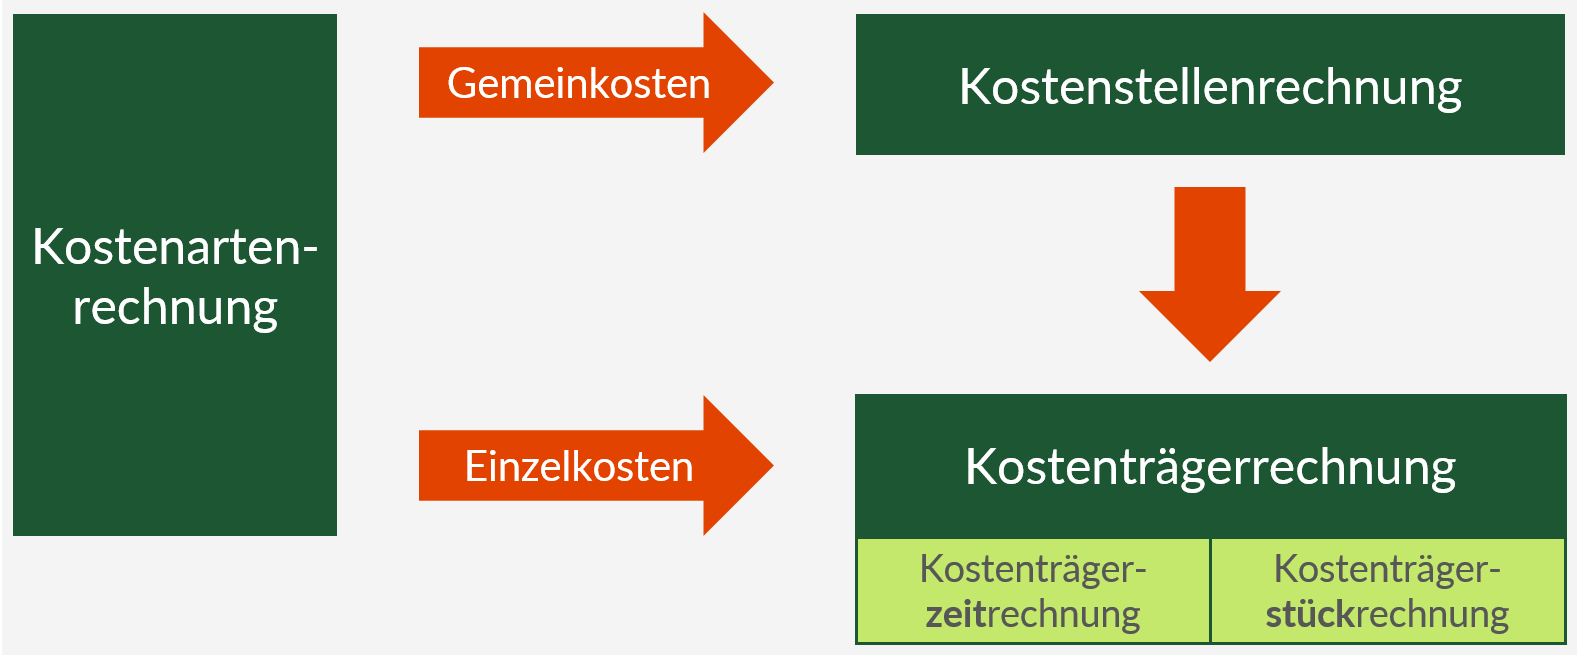
\includegraphics[keepaspectratio]{images/figure22.png}} \hfill{}

\caption{Abb. 2.2: Kostenrechnungsstufen im internen Rechnungswesen
(Trummer, o.J.). Quelle:
h\href{https://www.modu-learn.de/wordpress/wp-complete/uploads/2017/07/kostenanalyse-basis-neu.png}{ttps://www.modu-learn.de/wordpress/wp-complete/uploads/2017/07/kostenanalyse-basis-neu.png}}

\end{figure}%

Die~\emph{Kostenartenrechnung}~versucht, alle Kostenarten zu ermitteln,
, d. h. sie geht der Frage nach, welche Kosten insgesamt in der
Einrichtung anfallen. Dies sind z. B. Personalausgaben oder auch
Abschreibungen. In der~\emph{Kostenstellenrechnung}~gilt es zu
ermitteln, wo diese Kosten angefallen sind: in der Kindertagesgruppe, im
Einkauf, bei der Geschäftsleitung, in der Öffentlichkeitsarbeit oder an
sonstigen Stellen. Die~\emph{Kostenträgerrechnung}~beschäftigt sich mit
der Frage, wo die Kosten anfallen, also für welche Produkte und
Dienstleistungen. Da stellt sich die Frage, wie hoch die Kosten sind,
die im Rahmen einer Beratungsstunde, einer Betreuungsstunde oder ganz
allgemein im Rahmen eines Tagessatzes angefallen sind. Darunter lassen
sich alle Personalkosten fassen, also alle Sachkosten, die in
unterschiedlichen Kostenstellen angefallen sind. Sodann lässt sich
problemlos feststellen, wie „teuer'' eine Dienstleistung tatsächlich
ist.

\subsection{Phasen des Controllings}\label{phasen-des-controllings}

Im Controlling, wie vorangehend bereits ausgeführt, geht es um die
Aufgabe, klar zu planen und entsprechende Abweichungen frühzeitig
festzustellen, um daraus Maßnahmen abzuleiten. Hier sei ein Modell von
Bachmann (Bachmann 2008) angeführt, der sich mit den verschiedenen
Phasen des Controllings beschäftigt (vgl. \hyperref[figure23]{Abb.
2.3}).

\begin{figure}

\pandocbounded{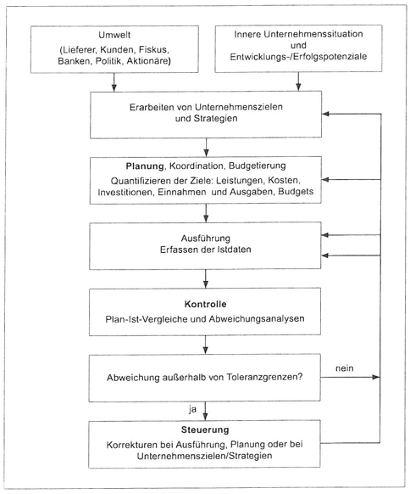
\includegraphics[keepaspectratio]{images/figure23.png}} \hfill{}

\caption{Abb. 2.3: Phasen des Controllings nach (Bachmann 2008, S. 9)}

\end{figure}%

Neben dem Controlling müssen am Anfang erstmal eine~\emph{Umweltanalyse
sowie unternehmensinterne Analysen}~durchgeführt werden, um
herauszufinden, mit welchen Stakeholdern überhaupt eine Verbindung
besteht. Es sind die Rahmenbedingungen der jeweiligen Situation zu
beschreiben. Anschließend wird daraus ganz allgemein die Zielstellung
für die Einrichtung herausgearbeitet, sodass dies zum Beispiel in
einem~\emph{strategischen Plan}~von Jahr zu Jahr erneuert werden kann.

Nach Festlegung der Zielstellungen geht es in der nächsten Phase um
die~\emph{Planung}~einer konkreten Wirtschaftsperiode. Dies kann bspw.
im Rahmen von Budgets oder mithilfe der Budgetierung getan werden, um
damit alle Kosten und Leistungen der Einrichtung geteilt oder nach den
Einrichtungsteilen gegliedert zu ermitteln.

Schließlich müssen im Laufe des Jahres die verschiedenen tatsächlich
angefallenen Kosten erfasst werden. Diese sind tabellarisch im Budget zu
erfassen. Mit diesem Wissen ausgestattet ist man in der Lage,
die~\emph{Kontrollmaßnahmen}~durchzuführen, ob sich bspw. Abweichungen
ergeben haben oder ob überhaupt Abweichungen entstanden sind.\\
\strut \\
Sofern~\emph{Abweichungen}~entstanden sind, muss überlegt werden, ob
diese vor dem Hintergrund definierter Toleranzgrenzen tolerierbar ist.
Wenn eine Kostenstelle leicht überzogen wurde, müssen nicht gleich die
härtesten Maßnahmen, wie z. B. ein Kostenstopp für alle zukünftigen
Anschaffungen ausgesprochen werden. Lohnsteigerungen im Umfang von 2 bis
4 \% sind beispielsweise etwas Normales. Dies kann sich durch
Tarifveränderungen oder eine Steigerung der Sozialabgaben ergeben haben.

Wenn allerdings die Toleranzgrenzen überschritten sind, dann müssen
entsprechende Veränderungsmaßnahmen eingeleitet werden. Dazu dient die
letzte Phase der~\emph{Steuerung}. Hier müssen Korrekturmaßnahmen
eingeleitet werden, damit die Ziele, die ursprünglich gesetzt worden
sind, auch erreicht werden können.

An der Seite sind verschiedene Pfeile erkennbar, die andeuten sollen,
dass hier verschiedene~\emph{Feedbackprozesse}~möglich sind. In der
ersten Phase widmet man sich kurzgesagt der~\emph{Planung}. Die zweite
Phase fragt danach, wie kontrolliert werden kann
und~\emph{Abweichungen}~ermittelt werden können. In der dritten Phase
beschäftigt man sich mit den
verschiedenen~\emph{Handlungsempfehlungen}~und Instrumenten, die
aufgetretenen Abweichungen wieder zu korrigieren.

\section{Personalmanagement}\label{personalmanagement}

Management ganz allgemein bedeutet: eine zielorientierte Gestaltung und
Steuerung von Organisationen. Beim Personalmanagement bzw. in der
Personalwirtschaft geht es darum, die Einrichtung durch Maßnahmen zu
gestalten, die darauf abzielen, einerseits neues Personal zu gewinnen,
das Personal zu verwalten bzw. zu erfassen und andererseits auch für die
Personalentwicklung der Mitarbeitenden aufzukommen (z.B. (Ribbeck 2020).
Das muss hinsichtlich wirtschaftlicher, sozialer und auch individueller
Zielsetzung geschehen. Es gibt ein umfangreiches Aufgabenpaket für das
Personalmanagement (vgl. \hyperref[figure24]{Abb. 2.4}).

\begin{figure}

\pandocbounded{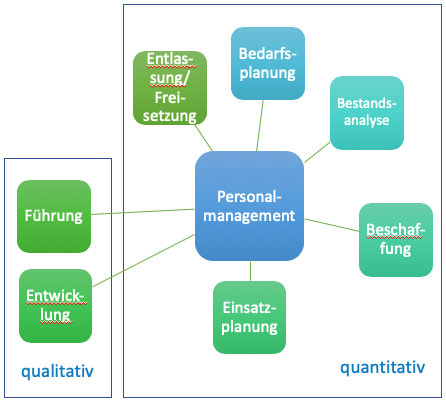
\includegraphics[keepaspectratio]{images/figure24.png}} \hfill{}

\caption{Abb. 2.4: Aufgabenfelder des Personalmanagements (in Anlehnung
an Hölzle 2006, S.18)}

\end{figure}%

Zunächst gibt es die Bedarfsplanung. Mit~\emph{Bedarfsplanung}~ist
gemeint, dass man sich Gedanken machen muss, wer mit welchen Kompetenzen
in welchen Betriebsteilen zukünftig eingeplant werden soll. Das
erfordert die regelmäßige Erfassung von Personalstatistiken und das
Sammeln von personenbezogenen Daten (\emph{Bedarfsanalyse}). Die
Beschaffung -- der Begriff kommt aus der Produktionswirtschaft -- meint
hier die Akquise von Personal. Das kann von außen geschehen, das kann
aber auch intern geschehen. Außen wäre beispielsweise die
Stellenanzeige, intern eine Umsetzung oder Veränderung von
Arbeitsverträgen.

Die~\emph{Einsatzplanung}~beschäftigt sich mit der Aufgabe, kurz- bzw.
mittelfristig Dienstpläne zu erstellen. Längerfristig ist die
Einsatzplanung zum Beispiel dazu wichtig, um Karrierewege planen zu
können.

Schließlich sind gelegentlich noch \emph{Entlassungen} und
\emph{Freisetzungen} durchzuführen. Für das Personalmanagement
gesprochen, handelt es sich bei Entlassungen um die Trennung von
Mitarbeitenden. Freisetzung ist ein Sammelbegriff dafür, dass es
alternative Maßnahmen gibt, die möglicherweise eine Entlassung
verhindern können oder vermeiden lassen, wie z. B. innerbetriebliche
Versetzungen, auch Umschulungen für eine andere Stelle, Kurzarbeit oder
auch Urlaub und Sonderurlaub.

Es gibt im Personalmanagement noch die Aufgabenbereiche
der~\emph{Führung}~und~\emph{Entwicklung}. Mit Führung ist gemeint, dass
jede Leitungskraft selbst reflektieren muss und entsprechendes Wissen,
Fähigkeiten und Erfahrungen besitzen muss, ein Team zu leiten, eine
Einrichtung zu leiten und Mitarbeitende zu motivieren. Sie muss auch
selbst in der Lage sein, das eigene Leitungshandeln zu hinterfragen.
Entwicklungsaufgaben ergeben sich durch die Personalentwicklung in den
Einrichtungen, d.~h. Kompetenzen müssen ständig weiterentwickelt und
durch geeignete Maßnahmen gewährleistet werden. Darunter fallen z. B.
Personalweiterbildungen.

Das Personalmanagement kann einerseits in
einen~\emph{quantitativen}~Teil (das sind die ersten fünf aufgeführten
Bereiche) und in einen~\emph{qualitativen}~Teil unterteilt werden (z.B.
Hölzle 2006).

\section{Organisationsentwicklung und
Change-Management}\label{organisationsentwicklung-und-change-management}

Zu diesem Funktionsbereich sei ein Modell der Organisationsentwicklung
bzw. des Change-Managements von Kurt Lewin angeführt. Dieser hat ein
Drei-Phasen-Modell entwickelt, welches mit der Metapher des Auftauens
und Einfrierens von Organisationsstrukturen argumentiert (vgl.
\hyperref[figure25]{Abb. 2.5}).

\begin{figure}

\pandocbounded{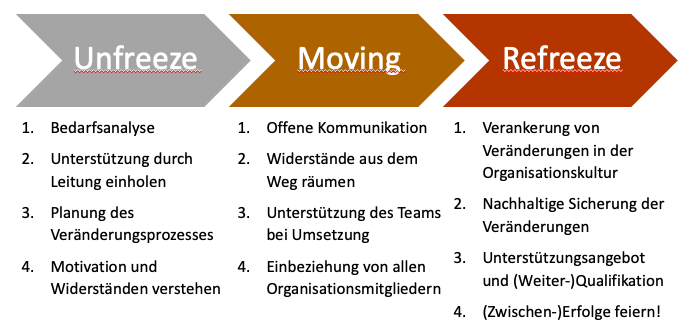
\includegraphics[keepaspectratio]{images/figure25.png}} \hfill{}

\caption{Abb. 2.5: Organisationsentwicklung und Change-Management nach
Kurt Lewins 3-Phasen-Modell (eigene Darstellung)}

\end{figure}%

In der ersten Phase, dem~\emph{Unfreezing}, geht es grundsätzlich darum,
den Bedarf und die Situation zu klären. Es muss ermittelt werden, was
verändert werden muss, wie dieser Prozess geplant werden kann, unter
welchen Umständen Mitarbeitende mitgenommen werden können und mit
welchen Widerständen ggf. gerechnet werden muss.

In der~\emph{Moving}-Phase geht es darum, offen zu kommunizieren, was
genau die Veränderung ist. Die Veränderungsprozesse müssen umgesetzt,
Widerstände behandelt und das Team regelmäßig einbezogen werden. Es sind
Fragestellungen und die dazugehörigen Lösungen zu entwickeln.
Letztendlich sollte regelmäßig über den aktuellen Stand in
Großgruppenveranstaltungen informiert werden.

In der~\emph{Refreezing}-Phase, dem Einfrieren, müssen die geänderten
Strukturen gefestigt werden. Es werden die neuen gefundenen Strukturen
und definierten Prozesse verankert. Das dient dazu, nachhaltig mit den
neuen Arbeitsstrukturen zu arbeiten und gegebenenfalls
Anpassungsqualifikationen durchzuführen. Wenn die Maßnahme erfolgreich
umgesetzt wurde, gilt es natürlich auch zum Schluss, den Erfolg zu
feiern.

\section{Sozio-Marketing}\label{sozio-marketing}

Schließlich gibt es noch den betriebswirtschaftlichen Funktionsbereich
des Marketings bzw. das~\emph{Sozio-Marketing}, also das Marketing
sozialer Einrichtungen.

\emph{Marketing}~ist zusammengefasst der Aufgabenbereich, der sich damit
beschäftigt, die jeweiligen Dienstleistungen und Produkte einerseits
hinsichtlich ihrer Qualität zu entwickeln und Werte zu schaffen sowie
andererseits zu kommunizieren sowie Kunden anzubieten und diese
Austauschbeziehung zu managen.

Nach Harald Christa (Christa 2010) ist~\emph{Sozio-Marketing}~„auf eine
konkrete Organisation der sozialen Arbeit bzw. der Wohlfahrtspflege
bezogen'', „umfasst weit mehr als rein kommunikationspolitische
Facetten'', „Anwendung der Denkweisen undInstrumente des Marketings in
und für soziale Organisationen'' (Christa 2010, S. 19, 24). Mithin
stellt sich die Aufgabe, die allgemeinen betriebswirtschaftlichen
Grundlagen des Marketings auf soziale Einrichtungen zu übersetzen.

Im Folgenden soll beispielhaft der \emph{Vier-Felder-Marketingmix}, ein
bekanntes Instrument des Marketings, vorgestellt werden. Dies ist dazu
geeignet, verschiedene Aufgaben bzw. Handlungsfelder des Marketings
zusammenzufassen, wobei unterschieden wird zwischen Leistungspolitik,
Preispolitik, Distributionspolitik und Kommunikationspolitik (vgl.
\hyperref[figure26]{Abb. 2.6}).

\begin{figure}

\pandocbounded{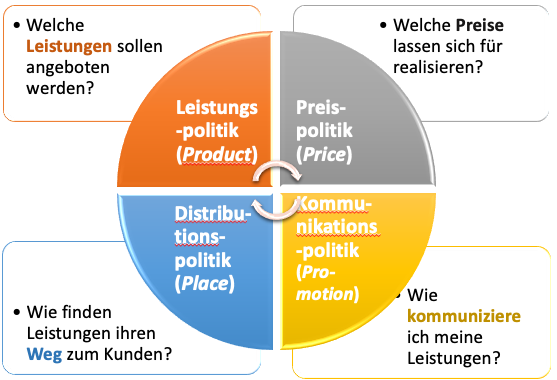
\includegraphics[keepaspectratio]{images/figure26.png}} \hfill{}

\caption{Abb. 2.6: Marketing-Mix (eigene Darstellung)}

\end{figure}%

In der~\emph{Leistungspolitik}~geht es um die Frage, welche Leistungen
überhaupt angeboten werden. Es muss ermittelt werden, wie die
marktgerechte Ausgestaltung der Leistung aussieht und welche Aussagen
sich von der Erhebung der Klient*innen- sowie Kundenbedarfe ergeben. Das
ist notwendig, um ermitteln zu können, ob die Qualität entsprechend gut
ist, sodass die Erwartungen der Kunden befriedigt werden. Des Weiteren
ist in Umwelt- oder Umfeldanalysen zu erforschen, wie sich das Produkt
bzw. die Dienstleistung von anderen unterscheidet. Eventuell ließe sich
eine Qualitäts- oder Kostenführerschaft übernehmen. Schließlich ist in
der Leistungspolitik auch eine „Unique selling proposition'' (USP) von
Bedeutung; ein Alleinstellungsmerkmal der Einrichtung muss
herausgearbeitet werden.

In der~\emph{Preispolitik}~geht es um die Frage, wie der Preis gestaltet
wird und wie sich Preise realisieren lassen. Darauf haben wir in der
Sozialwirtschaft weniger Einfluss, weil die Preise festgelegt sind, wenn
wir beispielsweise an die Leistungsentgelte denken, wobei diese Entgelte
im Regelfall feststehen. Nichtsdestotrotz müssen die Preise dahingehend
kalkuliert werden, wie z. B. durch eine Kostenanalyse soll ein Überblick
über die Kostenstruktur ermittelt werden. So muss ermittelt werden, wie
teuer eine Beratungsstunde oder ein Tagessatz ist. Wenn diese Berechnung
erfolgt ist, kann man in die Leistungsentgeltverhandlungen gehen und den
notwendigen Preis verlangen, damit alle Kosten der Einrichtung gedeckt
werden können. Es gibt ganz unterschiedliche Wege zur Preisfindung. Hier
wurde das Modell der Kostenorientierung vorgestellt. Man kann sich aber
auch bspw. bei der Kalkulation von Weiterbildungen an der Konkurrenz
orientieren. Man kann sich auch anhand der Nachfrage orientieren, also
dem Nutzer der jeweiligen Dienstleistungen. Darüber hinaus gibt es noch
das Target Costing, also die ziel- und nutzenorientierte Ermittlung von
Kosten bzw. Preisen. Die letztgenannten Verfahren sind eher im
Weiterbildungs- bzw. allgemein im Bildungsbereich passend.

Die~\emph{Distributionspolitik}~fragt danach, auf welchem Wege die
Leistungen zum Kunden gebracht werden. Es gibt sog. Absatzmittler wie z.
B. Schuldnerberatungen, die manchmal ein erster Anlaufpunkt für Menschen
in besonderen, finanziellen wie persönlichen Lebenslagen sind. Sie
können Menschen an andere Beratungen verweisen. Darüber hinaus gibt es
die Meinungsführer („Influencer''). Das sind diejenigen
meinungsbildenden Personen, die die Einrichtung kennen und
weiterempfehlen. Das können beispielsweise Selbsthilfegruppen, Elternrat
und Elterngruppen, aber auch andere Vereinigungen bzw.
Wohlfahrtsverbände sein, die auf unsere Einrichtung hinweisen. Die
Standortwahl ist ebenso ein Aspekt in Distributionspolitik. Es ist dabei
zu analysieren, wo sich die Einrichtung befindet: in einer Randlage oder
im Stadtzentrum. Davon hängt ab, welche Personen sie erreichen kann.
Schließlich sind die Öffnungszeiten sowie die Erreichbarkeit mit
öffentlichen Verkehrsmitteln entscheidend.

Den letzten großen Teil des Marketing-Mix stellt
die~\emph{Kommunikationspolitik}~dar. Hier geht es um die Frage, wie die
Leistungen kommuniziert werden können, sodass sie dann entweder die
gesamte Bevölkerung erreichen oder gezielt einzelne Gruppen ansprechen.
Es geht um die Erhöhung des Bekanntheitsgrades der Einrichtung in der
Öffentlichkeitsarbeit. Im Rahmen der Werbung müssen die
unterschiedlichen Kanäle und Medien gewählt werden: ob über Social
Media, über Werbung, über direkten Kontakt oder über eine Website.
Herausgearbeitet werden muss, mit welcher Botschaft man die Personen
erreicht, die man ansprechen will.

\section{Weitere Funktionsbereiche}\label{weitere-funktionsbereiche}

Abschließend ist ein Überblick über weitere Funktionsbereiche zu geben,
gewissermaßen die Balkone und das Dach des Hauses der BWL. Hierzu
erfolgt nur eine sehr sporadische Zusammenfassung in der folgenden
Abbildung. All diese Bereiche, die hier aufgeführt sind, haben eine
separate Veranstaltung im Laufe Ihres Studiums (vgl.
\hyperref[figure27]{Abb. 2.7}).

\begin{figure}

\pandocbounded{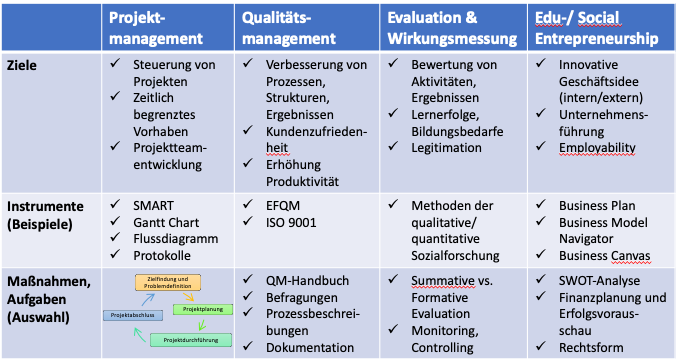
\includegraphics[keepaspectratio]{images/figure27.png}} \hfill{}

\caption{Abb. 2.7: Überblick weitere Bereich des Bildungsmanagements
(eigene Darstellung)}

\end{figure}%

Das~\emph{Projektmanagement}, darauf wurde bereits eingegangen, hat die
Aufgabe, Projekte zu steuern bzw. das Projektteam zu führen. Dabei
handelt es sich um befristete Maßnahmen. Am Anfang muss man sich
Gedanken über die Ziele zum Projekt machen. Es muss ein Plan entwickelt
werden, dieser umgesetzt sowie durchgeführt werden. Zum Schluss werden
die Ergebnisse veröffentlicht bzw. daraus ergibt sich möglicherweise ein
neues Thema, was in einem anderen Projekt umgesetzt werden kann. Die
smarte Zielformulierung kann hier als Instrument eingesetzt werden.
Ebenso können Charts dazu dienen, einen Projektplan zu entwickeln, aus
dem hervorgeht, zu welchem Zeitpunkt wann wer welche Tätigkeiten
übernimmt. Flussdiagramme sind hilfreich, um Prozesse zu beschreiben.
Zudem sind Protokolle von Meetings anzufertigen.

Das~\emph{Qualitätsmanagement}~hat die Aufgabe, Prozesse, Strukturen und
Ergebnisse regelmäßig zu überprüfen. Es bildet gewissermaßen einen
Garanten, um Standardisierung oder Professionalisierung zu ermöglichen.
In dessen Rahmen ist regelmäßig danach zu fragen, wie sich die
Kundenzufriedenheit darstellt und ob sich diese verändert hat. Umfassend
muss geprüft werden, wie die gesamte Einrichtung noch effektiver und
produktiver werden kann. Dazu gibt es verschiedene Modelle wie z. B. das
EFQM-Modell oder die DIN-ISO-Norm. Im Bereich der Sozial- und
Gesundheitswirtschaft gibt es noch zahlreiche andere Modelle und
Instrumente, die eingesetzt werden können. Im Qualitätsmanagement werden
verschiedene Maßnahmen festgelegt, Prozesse beschrieben und
dokumentiert, zudem sollte auch ein Qualitätsmanagement-Handbuch
entstehen.

Die~\emph{Evaluation bzw. Wirkungsmessung}~fragt danach, wie die
Aktivitäten und Ergebnisse, die sich im Rahmen der Tätigkeiten ergeben
haben, bewertet werden können. Zu ermitteln ist, was die Wirkungen sind,
die sich daraus ergeben und welche Effekte sich auf sozialer,
organisationaler und möglicherweise kommunaler sowie Sozialraumebene
ergeben. Sie dienen dazu, Lernerfolge, Bildungsbedarf und -veränderung
sowie Kompetenzentwicklungen abzubilden. In diesem Bereich nutzt man
Methoden der qualitativen und quantitativen Sozialforschung, um genau
diese Ergebnisbewertungen vorzunehmen. Die Evaluation hat das Ziel,
herauszufinden, wie die Ergebnisse der jeweiligen Maßnahme gegenüber
ihren Zielen zu einer wirkungsvollen Veränderung geführt haben. Die
formative Evaluation beschäftigt sich mit der schrittweisen und
begleitenden Evaluation und versucht, im Prozess eines Programms, einer
Maßnahme oder eines Projektes entsprechend durch Feedback und
Reflexionsmöglichkeiten auf den Verlauf von Monitoring- und
Controlling-Maßnahmen Einfluss zu nehmen. Die summative Evaluation
ermittelt die Wirkung nach Abschluss der Maßnahme.

Die~\emph{Evaluation bzw. Wirkungsmessung}~fragt danach, wie die
Aktivitäten und Ergebnisse, die sich im Rahmen der Tätigkeiten ergeben
haben, bewertet werden können. Zu ermitteln ist, was die Wirkungen sind,
die sich daraus ergeben und welche Effekte sich auf sozialer,
organisationaler und möglicherweise kommunaler sowie Sozialraumebene
ergeben. Sie dienen dazu, Lernerfolge, Bildungsbedarf und -veränderung
sowie Kompetenzentwicklungen abzubilden. In diesem Bereich nutzt man
Methoden der qualitativen und quantitativen Sozialforschung, um genau
diese Ergebnisbewertungen vorzunehmen. Die Evaluation hat das Ziel,
herauszufinden, wie die Ergebnisse der jeweiligen Maßnahme gegenüber
ihren Zielen zu einer wirkungsvollen Veränderung geführt haben. Die
formative Evaluation beschäftigt sich mit der schrittweisen und
begleitenden Evaluation und versucht, im Prozess eines Programms, einer
Maßnahme oder eines Projektes entsprechend durch Feedback und
Reflexionsmöglichkeiten auf den Verlauf von Monitoring- und
Controlling-Maßnahmen Einfluss zu nehmen. Die summative Evaluation
ermittelt die Wirkung nach Abschluss der Maßnahme.

In dieser Grundlagenveranstaltung wurden ausgewählte Funktionsbereiche
dargestellt, die in jeder Einrichtung eine Rolle spielen, unabhängig
davon, ob es sich um eine soziale oder um eine erwerbswirtschaftliche
Einrichtung im weitesten Sinne handelt.

\chapter{Organsationstheorie}\label{organsationstheorie}

\section{Was ist eine Organisation?}\label{was-ist-eine-organisation}

Im Folgenden werden wir uns mit dem organisationsbezogenen Management
beschäftigen und im Anschluss daran setzen wir uns mit verschiedenen
Managementkonzepten im Sozialmanagement (Teil 5) auseinander, die sich
insbesondere aus der öffentlichen Betriebswirtschaftslehre und dem
Non-Profit-Management ableiten lassen. Zunächst ist aber zu klären, was
Organisationen eigentlich sind und wie man diese sozialen Gebilde
beschreiben kann. Natürlich gibt es ganz unterschiedliche
Herangehensweisen und Aspekte, die wir einer Organisation bzw.
Organisationen zuschreiben können. Ein Aspekt der Organisation ist die
Koordination des Zusammenwirkens und die Ermöglichung einer inneren
Ordnung, wie unter anderem ihr Aufbau oder ihre Struktur. Prozesse
müssen definiert werden, es gibt feste Abläufe, es gibt
Verantwortlichkeiten und vieles mehr, das uns ermöglicht, koordinativ
zusammenzuwirken.

Darüber hinaus gibt es noch eine zweite Eigenschaft. Wir können
Organisationen als soziales System betrachten, die in einer Gesellschaft
ein Eigenleben besitzen. D. h. wenn eine Organisation gegründet wurde,
dann ist sie ein eigenes Objekt, ein abstraktes Gebilde, das in die Welt
gebracht wurde, welches wir für die Koordination nutzen können. Und man
kann es vielleicht daran erkennen, dass Organisationen bzw. Firmen
(rechtsdeutsch) auch Namen haben. Wir geben einer Organisation also
einen Namen, machen sie dadurch „persönlicher'' und direkter. Darüber
hinaus ist noch ein dritter Aspekt wichtig, wenn wir über Organisationen
sprechen: sie sind soziale Gebilde, die ein bestimmtes oder auch mehrere
Ziele verfolgen können. D. h. Organisationen ermöglichen ein
zielgerichtetes Handeln.

Stellen wir uns im Weiteren die Frage, was denn eine Organisation ist
bzw. was Organisationen ausmachen: Organisationen an sich umfassen
erstens eine Mehrzahl an Personen, die in dieser zusammenarbeiten. Der
Begriff ist so essenziell, dass wir häufig nach Synonymen ringen müssen,
weil wir einerseits Organisationen als Gebilde betrachten können, also
als abstrakte Einheiten. Andererseits ist die Organisation auch eine
Tätigkeit, nämlich etwas „zu organisieren'', z. B. die Durchführung
eines Projekts. Darüber hinaus kann man auf die Idee kommen, dass die
Menschen, die in Organisationen zusammenarbeiten, häufiger ihre Arbeit
im Sinne einer funktionalen Arbeitsteilung verrichten und eine
Organisation überhaupt erst eine Grundlage dafür schafft, dass man die
einzelnen Arbeitsprozesse aufeinander abstimmen und gleichzeitig
verschiedene Ziele verfolgen kann. D. h. es sind nicht nur mehrere
Personen, die zusammenarbeiten, sondern es gibt auch eine Koordination
der Zusammenarbeit. Zudem besitzen Organisationen jeweils eine Struktur
bzw. Hierarchie, die festgelegt werden muss. Es muss hierbei geklärt
werden, wer für was zuständig ist und entsprechend wer welche
Verantwortung(en) übertragen bekommt.

Schließlich kann man festhalten, dass Organisationen so etwas wie
soziale Systeme sind. Der Systembegriff taucht in ganz verschiedenen
Zusammenhängen im Laufe des Studiums der Sozialpädagogik und des
Sozialmanagements an mehreren Stellen auf. Letztgenannter Begriff hilft
zu beschreiben, wie Menschen miteinander zusammenwirken und wie
Zusammenarbeit überhaupt erst ermöglicht wird. Ich möchte erinnern an
die Unterschiede und Gemeinsamkeiten von Non-Profit- und
For-Profit-Organisationen nach Schwarz (1986), wo ebenfalls erwähnt
wurde, dass jede Organisation eine Art soziales System darstellt.

\section{Eigenschaften und Funktionen von
Organisationen}\label{eigenschaften-und-funktionen-von-organisationen}

Organisationen haben ganz verschiedene Funktionen. Sie dienen einerseits
der Überlebenssicherung, da sie für einen bestimmten Zweck gegründet
werden, um ein Ziel zu verfolgen; sie leisten damit für eine
Gesellschaft einen konkreten Beitrag in der Umsetzung bestimmter
Aufgaben. Darüber hinaus dienen sie dazu, wie oben bereits erwähnt, das
Zusammenleben zu organisieren und zu ordnen. Mit anderen Worten:
Organisationen werden ins Leben gerufen, um komplexe Problemstellungen
zu lösen, wozu eine Einzelperson möglicherweise nicht in der Lage wäre.

Gleichzeitig fungieren Organisationen bzw. ihre rechtsverbindlichen
Vertreter*innen häufig auch als Arbeitgeber und durch einen
Arbeitsvertrag wird das Überleben bzw. die Existenz der Mitarbeitenden
gesichert. Durch Organisationen wird also Arbeitsteilung ermöglicht.
Darüber werden Organisationen selbst als Objekte, als Entitäten
wahrgenommen, die mit anderen Organisationen zusammenarbeiten, etwa auf
Basis von Kooperationsverträgen. Sie treten dabei als Vertragspartner
auf, wenn sie eine eigene Rechtspersönlichkeit (= juristische Person,
gegenüber sog. natürlichen Personen nach Privat- oder öffentlichem
Recht) besitzen, z. B. Verein, Stiftung, GmbH.

Organisationen haben eine eigene Identität bzw. Persönlichkeit, die es
ermöglicht -- zumindest theoretisch -- eine Grenze zwischen dem Außen
und dem Innen zu ziehen. Nach außen hin erfolgt eine Abgrenzung zum
Wettbewerb und zu anderen nicht der Einrichtung Angehörigen. Nach innen
hin erfolgt es eine Sinngebung bzw. Zwecksetzung. Hier wird mit der
Organisation ein „Wir'' geschaffen. Dabei ist zu betonen, dass das Wir
ja durch einen Zusammenschluss von mehreren Menschen entstanden ist. Das
Wir bildet eine gewisse Gruppenidentität.

Menschen können ganz unterschiedliche Beziehungen zu Organisationen
aufbauen, z. B. können sie einer Organisation angehören. Damit werden
sie zu Mitgliedern der Organisation. Darüber hinaus gibt es aber auch
eine andere interessante Eigenschaft: Organisationen koordinieren auch
Menschen, z. B. indem bestimmte Ziele verfolgt und festgelegt werden,
was dazu führt, dass bestimmte individuelle Interessen bisweilen auch
zurückgesteckt werden müssen und dann sozusagen die Organisationsziele
im Vordergrund stehen.

Menschen passen sich in Organisationen über verschiedene Rollen und
Regeln an. Dann stellen sich Fragen wie z. B.: Was ist das richtige bzw.
anpasste Verhalten? Wie gehen wir aufeinander zu? Wie kommunizieren wir
mit unseren Stakeholdern? Was gibt es für Spielräume bzw. informelle
Regeln, die es zu beachten gilt? All das gehört u. a. zur
Organisationsstruktur und Organisationskultur, womit wir uns später
beschäftigen werden. Schließlich haben Organisationen, wie bereits
erwähnt, ein übergeordnetes Ziel: sie verfolgen eine Zweckrationalität.
Rationalität wird von ratio (lat. „Vernunft'', „Methode'') abgeleitet.
Zweckrationalität meint das Einrichtungsziel bzw. den Zweck der ggf. in
der Satzung einer Einrichtung definiert ist. Alle einer Organisation
angehörigen Mitglieder richten ihr Verhalten an den vorhandenen
Verantwortlichkeiten und Machtstrukturen aus. Solche Hierarchien werden
z. B. in Organigrammen festgelegt. Es gibt Befugnisse, die ausgesprochen
werden, und darüber hinaus ist natürlich auch die Verwirklichung der
persönlichen Ziele, Ideen und Interessen der Mitglieder von Bedeutung,
insbesondere wenn die eigenen Kompetenzen, Wissen und Fähigkeiten
weiterentwickelt werden sollen. Also kurz zusammengefasst geht es hier
darum, den Zweck und die Rationalität, für die die Einrichtung steht, zu
verwirklichen.

\section{Bilder von Organisationen}\label{bilder-von-organisationen}

Schauen wir uns im Folgenden verschiedene Bilder von Organisationen an.
Ich gehe hier auf einen Ansatz von Gareth (Morgan 1986; dt. Morgan 1997)
zurück, der in seinem gleichnamigen Buch Ende der 1980er Jahre von den
``Images of Organization'' gesprochen hatte. Zur Darstellung der
Geschichte der Organisationstheorie hat Morgan Metaphern verwendet. Vier
dieser Bilder, die unmittelbar interessant für unser Veranstaltungsthema
sind, seien im Folgenden einmal herausgegriffen, da sie uns ein besseres
Verständnis dafür liefern, wie sich die Idee von Organisationen im
Zeitverlauf entwickelt hat.

Erstens können Organisationen als Maschinen betrachtet werden. Hier
befinden wir uns im Zeitalter der Industrialisierung. Organisationen
sind Großunternehmen, die Massenprodukte in Fließbandarbeit herstellen.
Maschinen müssen regelmäßig geölt werden, um stets wie zwei Zahnräder
ineinandergreifen zu können. Eine Organisation funktioniert nur dann,
wenn auch das Räderwerk läuft. Diesem Bild einer Organisation liegt ein
mechanistisches Weltbild zugrunde, das natürlich dann später auch
kritisiert worden ist, z. B. mit Hilfe der Systemtheorie.

Organisationen können zweitens auch als Organismen bzw. lebende Systeme
angesehen werden. Damit ist gemeint, dass, wie im menschlichen Körper
bzw. anderen komplexen Organismen, die einzelnen Organe und Zellen
koordiniert miteinander zusammenarbeiten. Nicht jede Zelle hat die
gleiche Aufgabe, sondern es gibt ganz unterschiedliche Aufgaben, die von
Spezialisten in einem arbeitsteilig organisierten, wechselseitig
vernetzten System miteinander umgesetzt werden. Hier ist eine ganz
andere Metapher im Spiel, nämlich eine biologistische Sichtweise auf
Organisationen, was letztlich auch einen Ursprung der für die später
beschriebene Systemtheorie darstellt (z. B. Kybernetik). Im
metaphorischen Sinn des Organismus werden Organisationen als
funktionsfähige, soziale Systeme betrachtet.

Drittens können Organisationen auch mit der Metapher ‚Kultur'
beschrieben werden. Diese anthropologische, sozial- und
kulturwissenschaftliche Sichtweise besagt, dass Organisationen auf Basis
bestimmter Regeln, Werte und Normen aufgebaut sind und ihre Mitglieder
verschiedene soziale und funktionale Rollen einnehmen können. Letztlich
kann damit alle Eigenschaften, die allgemein dem abstrakten Phänomen
‚Kultur' zugeordnet werden können, auch auf das Zusammenwirken von
Menschen in Organisationen übertragen werden, z. B. dass die Mitglieder
in Organisation durch die Organisationskultur geprägt werden,
gleichzeitig aber auch die Mitglieder die Organisationskultur
entscheidend mitprägen.

Viertens können Organisationen auch im Sinne eines (psychischen)
Gefängnisses verstanden werden. Hierbei liegt eine psychoanalytische
Sichtweise zugrunde. Damit ist gemeint, dass alle Mitglieder einer
Organisation bestimmte Bedürfnisse und Befindlichkeiten, wie z. B.
Bedürfnisse nach Sicherheit, Anerkennung und Beteiligung, haben.
Insbesondere dann, wenn sich einzelne Individuen nicht unmittelbar mit
den organisationalen Zielen identifizieren können, z. B. weil es
persönliche Vorbehalte oder widersprüchliche Auffassungen gibt, kann
eine Organisation möglicherweise auch etwas erdrückend wirken.
Individuelle und organisationale Ziele können dabei nicht gleichzeitig
erreicht werden.

\section{St.~Galler Management-Modell der 3. Generation und seine
Erweiterungen}\label{st-galler-management-modell-der-3-generation-und-seine-erweiterungen}

\subsection{St.~Galler Management-Modell der 3. Generation nach
Rüegg-Stürm
(2003)}\label{st.-galler-management-modell-der-3.-generation-nach-ruxfcegg-stuxfcrm-2003}

In diesem ganzheitlichen und systemorientierten Modell wird eine
Organisation bzw. ein Unternehmen eingebettet in Ihrer Systemumwelt
dargestellt (vgl. Rüegg-Stürm 2003). Das Modell ist wie in
\hyperref[figure31]{Abb. 3.1} aufgebaut.

\begin{figure}

\pandocbounded{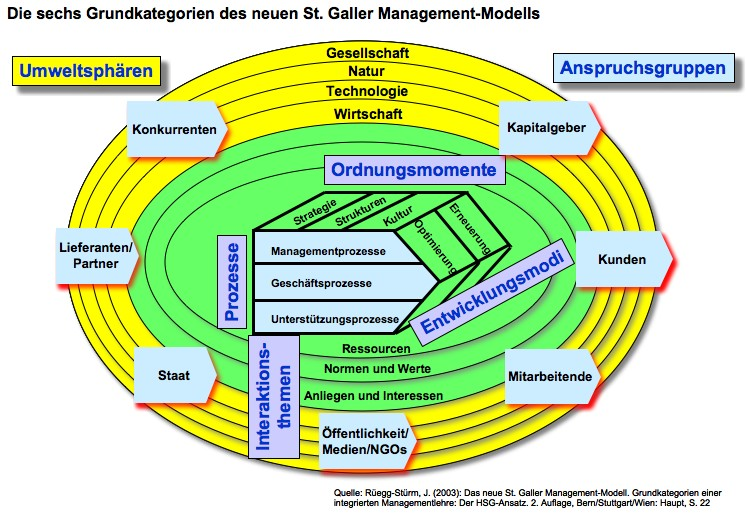
\includegraphics[keepaspectratio]{images/figure31.jpeg}} \hfill{}

\caption{Abb. 3.1: Grundkategorien des SGMM (Rüegg-Stürm 2003, S. 22),
Quelle: \url{https://de.wikipedia.org/wiki/Datei:SGMM2.jpg} (CC Public
Domain)}

\end{figure}%

Auf den äußeren Schalen gibt es die sog. Umweltsphären. Dies bilden die
Rahmenbedingungen, in denen sich Organisationen bewegen und bewähren
müssen. Dazu gehören beispielsweise gesellschaftliche Prozesse, z. B.
Teilhabe, Partizipation und Sozialgesetzgebung, ebenso aber auch die
natürlichen (z. B. nachhaltiges Wirtschaften), technologischen und
wirtschaftlichen Rahmenbedingungen bzw. die Sozialwirtschaft im Ganzen
gesehen. In diesen Umweltsphären und mit der Organisation unmittelbar in
Beziehung stehend gibt es verschiedene Anspruchsgruppen, die sogenannten
Stakeholder.

Bei den Stakeholdern kann es sich um Einzelpersonen oder auch Gruppen
handeln. Der Staat gibt bspw. die gesetzlichen Rahmenbedingungen vor,
nach denen wir uns zu orientieren haben. Die Lieferanten stellen uns
bestimmte Produkte oder auch Dienstleistungen zur Verfügung, sodass eine
Einrichtung überhaupt erst einmal betrieben kann. Organisationen stehen
darüber hinaus in Konkurrenz bzw. Wettbewerb mit anderen Einrichtungen,
die ähnliche Produkte und Dienstleistungen anbieten. Bei den
Kapitalgebern können wir etwa an die Leistungs- bzw. Kostenträger in der
Sozialwirtschaft denken, die soziale Dienstleistungen finanzieren. Es
gibt Kund*innen bzw. Klient*innen, für die wir unsere Dienste anbieten
und schließlich gibt es die Mitarbeitenden, die innerhalb einer
Einrichtung dafür verantwortlich sind, dass der Zweck verfolgt wird,
alle notwendigen Aufgaben erledigt und die Qualität des Angebots
weiterentwickelt wird. Eine Austauschbeziehung besteht regelmäßig auch
mit der Öffentlichkeit, den Medien und Nichtregierungsorganisationen (z.
B. Gewerkschaften). Alle diese Stakeholder haben verschiedene Aufgaben
bzw. tragen verschiedene Interessen und Erwartungen an die Einrichtung
heran. Dies wurde bereits weiter oben bei dem Konzept der
Multirationalität angesprochen. Mit anderen Worten handelt es sich bei
dem St.~Galler Management-Modell um ein stakeholderorientiertes Konzept.

In der Mitte der Grafik befindet sich schließlich die Organisation
selbst, die über sog. Interaktionsthemen, dargestellt auf den inneren
Kreisen, mit den Stakeholdern verbunden sind. Zu diesen Austauschthemen
gehören bspw. Ressourcen, Normen und Werte sowie Anliegen und
Interessen. Mit Ressourcen ist gemeint, dass hier sozusagen personelle,
finanzielle und sachliche Ressourcen zur Verfügung gestellt werden
müssen, damit die Einrichtung funktioniert. Denn jede Einrichtung
benötigt Personal und finanzielle Mittel, Gerätschaften, ein Gebäude
bzw. Räumlichkeiten. Darüber hinaus gibt es Normen und Werte, die
grundlegend für die Zusammenarbeit gelten, z. B. professioneller
Anspruch gegenüber den Klient*innen, Kommunikationsregeln innerhalb der
Einrichtung. Außerdem gibt es verschiedene Anliegen und Interessen der
einzelnen Stakeholder, die aufgenommen bzw. bearbeitet werden müssen, z.
B. finanzielle Interessen, Kooperationen mit anderen Einrichtungen,
Kompetenzentwicklung der Mitarbeitenden.

Im Mittelpunkt der Grafik steht die als Pfeil dargestellte Organisation
selbst, dort werden die sog. Ordnungsmomente beschrieben, u. a.
Organisationsstrategie, Organisationsstruktur und die
Organisationskultur. Auf der Strategieebene geht es um die allgemeinen
und spezifischen Zielsetzungen und strategische Pläne innerhalb von
Organisationen. Mit Hilfe der Organisationsstruktur wird die Frage
geklärt, wie Organisationen aufgebaut sein müssen, z. B. in Form eines
Organigramms. Bei der Organisationskultur steht die Frage im
Vordergrund, wie wir in der Einrichtung miteinander zusammenarbeiten,
welche Werte wir teilen und welche Gepflogenheiten und Verhaltensweisen
existieren. Auf der Vorderseite des als Pfeil dargestellten Unternehmens
sehen wir verschiedene Prozesse, die innerhalb von Organisationen
ermöglicht werden sollen. Dazu gehören Managementprozesse, wozu
verschiedene Leitungs- und Führungsaufgaben wie Personalentwicklung,
Controlling und Geschäftsführung zählen. Die Geschäftsprozesse umfassen
demgegenüber alle alltäglichen Aufgaben bis hin zur Tagesplanung. Mit
Unterstützungsprozessen sind solche Prozesse gemeint, die die
Einrichtung in die Lage versetzen, den alltäglichen Betrieb zu
organisieren, z. B. Reinigungsdienste und Essensversorgung.

An der Pfeilspitze gibt es die sog. Entwicklungsmodi. Damit ist gemeint,
dass sich jede Organisation kontinuierlich weiterentwickeln muss. Dies
kann durch Erneuerungs- und Optimierungsprozesse geschehen. Optimierung
heißt, dass man dabei einerseits kleine Schritte gehen und Schritt für
Schritt Veränderungen umsetzen kann, während die Erneuerung eine
radikale Unternehmenstransformation darstellt, welche möglicherweise mit
Brüchen und einer neuen Unternehmensphilosophie einhergehen kann.

Alle weiteren Ausführung in diesem Abschnitt des organisationsbezogenen
Managements sind entsprechend der verschiedenen Ebenen und Aspekte des
St.~Galler Management-Modells der dritten Generation strukturiert.
Ausführlicher wird sich dann mit dem Strategieprozess, der Struktur- und
Prozessperspektive, Organisationskultur und der Organisationsentwicklung
beschäftigt.

\subsection{Systemisch-reflektiertes Management-Modell nach Lambers
(2015)}\label{systemisch-reflektiertes-management-modell-nach-lambers-2015}

Eine Erweiterung bzw. Übersetzung des St.~Galler Management-Modells
dritter Generation hat Lambers (Lambers 2015) in Form seines sog.
\emph{Systemtheoretisch-reflektierten Managementmodells (SRM)}
vorgenommen. Dabei wurde versucht, das Modell für soziale Einrichtungen
zu konkretisieren. Auf der äußeren Schale, der Umweltsphären, sind
verschiedene Rahmenbedingungen und Kontexte der Sozialen Arbeit
hervorgehoben, z. B. Familie, Politik, Recht, Erziehung, Medien,
Massenmedien, Wissenschaft und Wirtschaft. Diese bilden gewissermaßen
die Grundkontexte und Ausgangsbedingungen, in denen sich soziale
Organisation befinden bzw. bewähren müssen. Der innere, dunkelgrau
dargestellte Kreis beinhaltet die verschiedenen Normen, Werte,
Ressourcen und Interessen, welche für den Austausch zwischen den
verschiedenen Stakeholder und der Einrichtung von Bedeutung sind: z. B.
Geschäftsführung, Aufsichtsorgane, Netzwerke, Kooperationspartner,
Konkurrenten, Aufsichtsbehörden, Kosten- bzw. Leistungsträger. Außerdem
gibt es noch andere Adressaten, Angehörige, Berater*innen und
Mitarbeitende, die als Stakeholder eine bedeutende Rolle spielen können.
Mit der Blackbox ist gemeint, dass es möglicherweise noch weitere
Beteiligte geben kann, die uns aber aktuell nicht bekannt sind und ggf.
mit einer Stakeholderanalyse erst ausfindig gemacht werden müssen. Im
Zentrum des Modells steht wie auch im Originalmodell die Organisation
selbst. Die Ordnungsmomente sind gleich dargestellt. Neu sind neben den
Management-, Geschäfts- und Unterstützungsprozessen die sog.
Vernetzungsprozesse. Damit ist gemeint, dass es auch zur allgemeinen
Aufgabenstellung für Einrichtungen der sozialen Arbeit gehört, die
Vernetzung zwischen und mit anderen Einrichtungen herzustellen und zu
pflegen, z. B. Grundschule, Hort und Kita.

\chapter{Strategieebene}\label{strategieebene}

\section{Strategieentwicklung}\label{strategieentwicklung}

Im Folgenden betrachten wir zunächst einmal detaillierter das
Ordnungsmoment der Strategieentwicklung. Insbesondere gehen wir dabei
auf das Leitbild als Bestandteil der strategischen
Unternehmensentwicklung ein. Nach Giesel (2007) kann der
Strategieentwicklungsprozess anhand der Ebenen normatives, strategisches
und operatives Management beschrieben werden. Auf der normativen
Managementebene wird die unmittelbare Zwecksetzung der Einrichtung
festgelegt, warum und für was die Einrichtung gegründet wurde. Die
strategische Ebene beschäftigt sich mit der Frage, welche Ziele denn
formuliert werden müssen, damit die Unternehmensphilosophie bzw. die
Zweckbestimmung der Einrichtung überhaupt sinnvoll erreicht werden kann.
Das operative Management auf der untersten Ebene ist gewissermaßen das
Alltagsgeschäft. Dabei geht es darum, die gesetzten Ziele umzusetzen, um
dann am Ende des Jahres zu überprüfen, ob die Ziele schließlich erreicht
worden sind.

Den einzelnen Managementebenen lassen sich schließlich die verschiedenen
Aufgaben im Rahmen der Strategieentwicklung zuordnen. Auf normativer
Ebene muss die Unternehmensphilosophie und Unternehmenspolitik, also das
grundlegende Ziel formuliert werden. Das Leitbild, in der Mitte als
Pfeil dargestellt, bildet gewissermaßen das grundlegende Konzept bzw.
das integrative Verbindungsglied zwischen dem normativen, strategischen
und operativen Management. Auf normativer Ebene wird festgelegt, was die
vertretenen Werte und Überzeugungen der Organisation sind, welche
Aufträge verfolgt werden, wie die Zusammenarbeit gestaltet werden soll.
Auf strategischer Ebene muss in Programmen konkretisiert werden, wie die
Unternehmensphilosophie in der jeweiligen Planungsperiode umgesetzt
werden soll. Die Organisation hat verschiedene Aufträge zu erfüllen und
in Form von sog. Programmen bzw. Plänen ist längerfristig der
Arbeitsprozess und die Geschäftsentwicklung zu planen. Für die
Wirtschaftsplanung kann man sich hier beispielsweise die Aufstellung
eines Planbudgets vorstellen, was die Bewirtschaftung aller verfügbaren
Ressourcen beinhaltet, die zur Verwirklichung der Strategien dienen
können. Schließlich auf der untersten Ebene müssen die einzelnen
Aktivitäten, die einzelnen Prozesse, ob dies nun Management-,
Geschäfts-, Unterstützungs- oder Vernetzungsprozesse sind, für die
jeweiligen Planungsperiode organisiert werden.

\section{Leitbilder}\label{leitbilder}

\subsection{Funktionen von
Leitbildern}\label{funktionen-von-leitbildern}

Das Leitbild beschreibt den Auftrag bzw. die Vision einer Einrichtung:
Für welche Zwecke sind wir gegründet worden, wer arbeitet in unserer
Einrichtung, welche Werte verfolgen wir, wie wollen wir uns entwickeln?
Das Leitbild ist der Ausgangspunkt für die gelebte Kultur in der
Einrichtung, die meistens auch in Form von Mission Statements, also
formulierten Leitbilder, festgeschrieben ist, die die grundlegenden
Prinzipien des Auftrags einer Einrichtung beinhalten. Ein Leitbild
sollte auf ganz unterschiedliche Art und Weise wirken: Es wirkt nach
außen, indem damit die Öffentlichkeit informiert wird, und nach innen,
indem es eine Orientierung und Motivation für die Mitarbeitenden und
Führungskräfte bzw. Stakeholder der Organisation bildet. Zweitens gibt
das Leitbild auch einen Rahmen dafür vor, Strategien und Ziele der
Einrichtung wie in den operativen bzw. alltäglichen Aufgaben umgesetzt
werden können. Die drei genannten Punkte sind schließlich Ausgangspunkte
dafür, um überhaupt erstmal eine strategische Planung,
Personalentwicklung und Öffentlichkeitsarbeit umsetzen zu können. Nach
innen und nach außen wirken Leitbilder dahingehend, dass eine
Organisationsidentität geschaffen wird, also ein Selbstverständnis
entwickelt wird, wie mit Mitarbeitenden gemeinsam gesetzte Ziele
erreicht werden sollen. Drittens dient das Leitbild auch dazu, die
Ziele, die gesetzt wurden bzw. die Vision, die beschrieben worden ist,
in die Tat umzusetzen, zu planen und zu steuern.

\subsection{Begriffliche Einordnungen}\label{begriffliche-einordnungen}

Den Begriff Leitbild kann man ganz unterschiedlich einordnen und es gibt
verschiedene konkurrierende Bedeutungen, die im Folgenden differenziert
werden sollen. Leitbilder sind schriftliche Fixierungen der Vision und
Mission einer Einrichtung, bilden Werte und Grundsätze für das Handeln.
Sie müssen Antworten auf Fragen antworten wie z. B. Wer sind wir?, Wo
stehen wir? und Was zeichnet uns aus? Darüber hinaus gilt es von der
Strategie- und Zielebene immer die konkrete Maßnahmenebene abzugrenzen:
Auf der Zielebene müssen die Fragen beantwortet werden: Wo wollen wir
hin? Was wollen wir erreichen? Werte, die Vision und Grundsätze müssen
übersetzt werden in operationalisierbare Zielformulierung. Schließlich
müssen strategische Überlegungen konkretisieren, wie die gesetzten Ziele
erreicht werden können. Auf der Maßnahmenebene ist zu klären, was wir
denn konkret dafür tun müssen, damit die Strategien umgesetzt werden,
die Ziele erreicht und das Leitbild bzw. die gesetzten Werte und die
Vision umgesetzt werden.

\subsection{Fragen für die
Leitbildentwicklung}\label{fragen-fuxfcr-die-leitbildentwicklung}

Im Rahmen der Leitbildentwicklung ist es empfehlenswert, sich
verschiedene Fragen zu stellen, deren Antworten letztendlich Bestandteil
des Leitbilds werden können. Entsprechend der Übersicht von Graf and
Spengler (2013) können wir dabei verschiedene Fragekomplexe
unterscheiden. Erstens geht es im Leitbild darum, den Auftrag, die
Identität und Geschichte der Organisation zu beschreiben, d.~h. Fragen
zu klären, wie z. B. wer wir sind und woher wir kommen. Das ist die
Präambel eines jeden Leitbilds. Darüber hinaus kann man sich zweitens
die Fragen stellen, was wollen wir, also konkret: Welchen Anspruch
verfolgen wir? bzw. Was sind die Werte und Überzeugungen? Kurz
zusammengefasst: Was ist die Philosophie der Einrichtung? Grundlegend
ist die Frage zu klären: Wie erfüllen wir diesen Auftrag, den wir vorher
definiert haben? Drittens gilt es folgende Fragen zu bearbeiten:Was tun
wir, für wen sind wir da und mit wem arbeiten wir zusammen? Damit wird
näher beschrieben, welche Leistungen eine Einrichtung anbietet und wer
zur Zielgruppe gehört. Viertens gibt auch Fragestellungen hinsichtlich
des lokalen, nationalen und globalen sowie politischen und sozialen
Umfelds zu klären: Wo arbeiten wir? Was ist unser Einzugsgebiet,
entweder lokal und in der Kommune oder arbeiten wir möglicherweise
bundesweit oder haben wir auch Klienten und Partner im europäischen
Ausland oder im weltweiten Kontext. Welche politischen und sozialen
Rahmenbedingungen prägen unsere Arbeit. Fünftens sollte sich auch mit
dem Qualitätsanspruch sowie fachlich-professionellen Verständnis
auseinandergesetzt werden. Dabei stehen folgende Fragen im Mittelpunkt:
Wie arbeiten wir? Was können wir? Was können besser als andere
Einrichtungen. Sechstens geht es um die Frage, wie wir miteinander
umgehen. Dabei steht die Frage nach der Organisationskultur im
Vordergrund: Wie wird kommuniziert? Wie werden Kooperationen und
Partnerschaften gelebt? Welche Grundsätze und Prinzipien gelten für die
Leistungserfüllung? Wie wird Führung gelebt? Und schließlich siebtens
gilt es die Frage zu beantworten: Wer sind unsere Kooperationspartner?
Wer sind unsere Förderer?

\subsection{Leitbildentwicklung}\label{leitbildentwicklung}

Nachdem näher beschrieben wurde, was Leitbilder sind und welche
vielfältigen Funktionen sie besitzen, wird im Folgenden auf deren
Gestaltung bzw. partizipative Entwicklung näher eingegangen. Im ersten
Schritt muss man einen Projektplan und Skizze für den Prozess der
Leitbilderstellung aufstellen, worin ein Zeitplan, die zur Verfügung
stehenden Ressourcen und das methodische Vorgehen dargestellt wird.
Zweitens muss eine Arbeitsgruppe gebildet werden, der möglichst
verschiedene Stakeholder angehören, z. B. Leitungskräfte, Mitarbeitende
und gegebenenfalls ehrenamtlich Mitarbeitende und Klienten*innen. Die
Arbeitsgruppe kann auf Basis einer Stakeholderanalyse zusammengestellt
werden. Im Rahmen des dritten Schrittes, der IST- bzw. Situationsanalyse
ist sich ein Überblick über die Rahmenbedingungen zu verschaffen,
Antworten auf die oben genannten Fragen zu finden und anschließend aus
dem Brainstorming eine Liste möglicher Ideen für das Leitbild zu
entwickeln. Aus der IST- und Situationsanalyse ist viertens ein erster
Soll-Entwurf abzuleiten, der eine Zusammenfassung und Beantwortung der
genannten Fragen darstellt. Der Entwurf wird im fünften Schritt allen
Mitgliedern der Einrichtung vorgestellt und diskutiert. Aus der
Diskussion wird sechstens ein zweiter überarbeiteter Entwurf entwickelt.
Ggf. ist dieser Schritt mehrmals zu wiederholen bis im achten Schritt
der Revisionsprozess abgeschlossen werden kann und das Leitbild
verbindlich verabschiedet wird. Verabschiedet meint hier, dass das
einerseits durch den Vorstand genehmigt und gleichzeitig, wenn
vorhanden, mit der Arbeitnehmer*innenvertretung abgestimmt werden muss.
Der Abschluss des Leitbildungsprozesses ist schließlich Ausgangspunkt
für den nächsten Leitbilderstellungsprozess bzw. die
Leitbildüberarbeitung. In den Qualitätszirkeln bzw. in den in der
Einrichtung stattfindenden Sitzungen sollte darauf geachtet werden, dass
das Leitbild regelmäßig fortgeschrieben wird.

\subsection{Qualitätskriterien für die
Leitbildentwicklung}\label{qualituxe4tskriterien-fuxfcr-die-leitbildentwicklung}

Wie können Leitbilder hinsichtlich ihrer Qualität eingeschätzt werden?
Für Antworten auf diese Fragen ist der Ansatz von Maak and Ulrich (2007)
hilfreich. Zunächst kann erstens geprüft werden, ob das Leitbild
inklusiv genug formuliert wurde, also alle Beteiligten in der
Organisation gleichermaßen anspricht, sie alle mitnimmt und für alle
anwendbar ist. Zweitens ist zu prüfen, wie glaubwürdig das Leitbild ist.
D. h. ist das Leitbild realistisch formuliert? Steht es im Einklang mit
den vom Träger gelebten Werten und inwieweit lässt es sich umsetzen?
Drittens geht es um die Frage der Zielformulierung: Sind die
formulierten Ziele erstrebenswert bzw. motivierend, sodass alle
Beteiligten an der Erfüllung der Ziele mitarbeiten können? Mit dem
Kriterium ‚Klarheit' fragen wir viertens danach, inwieweit und wie
präzise das Leitbild formuliert wurde. Floskeln sind ebenso zu vermeiden
wie hochtrabende Fachsprache. Das Leitbild ist verständlich für eine
breite Leserschaft zu formulieren. Eine separate Ausgabe in einfacher
Sprache ist ebenfalls empfehlenswert. Schließlich geht es fünftens um
die Konkretheit des Leitbilds: Ermöglicht das Leitbild die Umsetzung und
Erfüllen der konkreten Ziele? Ist es kontrollier-, überprüf- und
einlösbar? Zur Prüfung der Konkretheit kann die SMART-Technik eingesetzt
werden.

\subsection{Beispiele für Leitbilder}\label{beispiele-fuxfcr-leitbilder}

Abschließend sollen einige ausgewählte Leitbilder präsentiert werden,
die im Rahmen eines zurückliegenden Projekts zur Analyse der
Profilbildungen in diakonischen Sozial- und Gesundheitsunternehmen
gesammelt wurden (vgl. Arnold et al. 2017). Es lassen sich verschiedene
Ausgestaltungsformen finden. Ein Leitbild kann beispielsweise als
Wordcloud dargestellt werden (z. B. Diakonie Bautzen). Ein Leitbild kann
anhand verschiedener Leitsätze zusammengesetzt werden, wie bei der
Diakonie am Thonberg. Die Leitsätze helfen zu übersetzen, was die
Einrichtung für Ziele verfolgt und nach welchen Prinzipien sie arbeitet.
Schließlich kann in Form einer Grafik der Strategieentwicklungsprozess
dargestellt, der von der Vision über die strategische Ausrichtung, die
Ziele bis zur Umsetzung reicht. Im Leitbild der Diakonie -- Stadtmission
Dresden wird beispielsweise der Versuch unternommen, die verschieden
Managementebenen abzubilden: Auf der normativen Ebene findet sich die
Vision der Einrichtung und auf der strategischen Ebene die mehrere
Wirtschaftsperioden überdauernde Grundausrichtung. Auf der Zielebene
gilt es, die Grundausrichtung in Strategien für die einzelnen
Leistungsbereiche zu übersetzen. Schließlich müssen auf operativer Ebene
die gesetzten Zielstellungen entsprechend umgesetzt werden. Am Ende
eines jeden Berichtsjahres ist zu überprüfen, ob die jeweiligen
geplanten Ziele tatsächlich erreicht wurden. So schließt sich dann der
Kreislauf vom operativen zum strategischen und zum normativen
Management.

\chapter{Struktur- und
Prozessperspektive}\label{struktur--und-prozessperspektive}

Auf dieser Ebene des organisationsbezogenen Managements stehen die
Abläufe und der Aufbau der jeweiligen Organisationen im Mittelpunkt. Im
Folgenden beschäftigen wir uns zunächst mit den wichtigsten
Grundbegriffen. Danach wird anhand verschiedener praktischer Beispiele
gezeigt, wie die Aufbaustruktur in Form von Organigrammen umgesetzt oder
beeinflusst werden kann. Auf der prozessbezogenen Ebene werden zwei
Instrumente eingeführt, die uns in die Lage versetzen, Abläufe zu
steuern.

\section{Grundbegriffe}\label{grundbegriffe}

Wenn wir von der Aufbauorganisation sprechen, dann sind Organigramme als
Modelle von Organisationen gemeint. Organigramme ermöglichen die
Darstellung und Definition nicht nur der Struktur der Organisation,
sondern auch der Aufgabenverteilung und der
Verteilungsverantwortlichkeiten. Darüber hinaus gibt es die
Ablauforganisation, die die organisationsinternen Prozesse in den Blick
nimmt. Wir versuchen, mit Hilfe der Ablauforganisation die Verteilung
und Vernetzung von verschiedenen Aufgaben innerhalb der Einrichtung zu
modellieren und zu entwickeln und klären dabei die Fragen: Wer hat
welche Aufgaben in welchem Bereich und wie werden diese Aufgaben dann
jeweils mit welcher Verantwortung umgesetzt? Gibt es so etwas wie
Aufgaben- und Tätigkeits- bzw. Stellenbeschreibungen, die in
Zusammenhang mit der Erfüllung des Arbeitsvertrags stehen? Warum
brauchen wir das?

Während der Strategiebildung und -entwicklung -- womit sich der
vorangegangene Abschnitt beschäftigt hat und wo auch auf die zukünftige
Entwicklung der Einrichtung eingegangen wurde -- haben wir es hier mit
dem formalen Teil des organisationsbezogenen Managements zu tun. Wir
brauchen klare Rollendefinitionen, Entscheidungsstrukturen und
Kommunikationswege damit die Organisation und ihre Mitglieder effizient
und effektiv arbeiten können.

\section{Organigramme}\label{organigramme}

\subsection{Was sind Organigramme?}\label{was-sind-organigramme}

Im Rahmen von Organigrammen können die vertikalen und horizontalen
Strukturverhältnisse bzw. der Aufbau der Organisation dargestellt
werden. Ein Organigramm ist eine strukturelle Übersicht über die
verschiedenen betrieblichen Bereiche und Funktionen bzw. Aufgaben, die
in einer Einrichtung existieren. Der Prozess zur Definition einer
Aufbauorganisation für eine kommunale Einrichtung läuft beispielsweise
wie folgt ab: Zunächst beginnt man mit einer Aufgabenbeschreibung und
einem Aufgabengliederungsplan für jeden Bereich, woraus durch
Aggregation der verschiedenen Teilpläne ein Verwaltungsgliederungsplan
aufgestellt wird. Ein Dezernatsverteilungsplan hat die Funktion, alle
innerhalb eines Geschäftsbereiches (Dezernate) existierenden
Verwaltungseinheiten zusammenzufassen. Wenn wir anschließend alle
Dezernate der kommunalen Verwaltung zusammen, kann ein
Geschäftsverteilungsplan entwickelt werden, der uns in die Lage
versetzt, spezifische Entscheidungsbefugnisse zu definieren. Der
Geschäftsverteilungsplan wird schließlich angereichert durch
Informationen aus der Personalabteilung, wie z. B. Stellenpläne, und
stellt den Ausgangspunkt für die Organigramme dar. Mit anderen Worten
wird die Struktur des Hauses, letztendlich im Geschäftsverteilungsplan
dargestellt. Bei der Erstellung von Stellenbeschreibungen kann darauf
zurückgegriffen werden, um zu definieren, welche Personen innerhalb
dieser Gesamthierarchie einer Einrichtung was zu tun haben.

Im Folgenden werden die verschiedenen Organigramme vorgestellt sowie auf
deren Vorteile und Nachteile eingegangen.

\subsection{Einlinienorganisation}\label{einlinienorganisation}

Bei der Einlinienorganisationen ist die Verantwortung bzw. Aufteilung
der Organisation entlang einer vertikalen Struktur organisiert. Oben
angeordnet ist die Unternehmensleitung, die verantwortlich ist für die
Steuerung und für die Organisation der verschiedenen Bereiche. Wie in
\hyperref[figure32]{Abb. 3.2} dargestellt, werden im Organigramm
unterhalb der Unternehmensleitung die verschiedenen Hauptabteilungen und
möglicherweise noch ein Projektbereich erfasst. In den einzelnen
Hauptabteilungen gibt es auch noch eine klare Untergliederung in
einzelne Unterabteilungen bzw. in Teilprojekte. Im Ganzen gesehen ist
alles sprichwörtlich wie an einem Faden aufgehängt. Alles wird dirigiert
von der obersten Instanz bzw. von den jeweiligen unteren Instanzen, den
Hauptabteilungen.

Ein Vorteil dieser Organisationsstruktur ist, dass es sehr klar
gegliedert und übersichtlich ist. Ein Nachteil könnte sein, dass hier
insbesondere in Entscheidungsprozessen immer erst noch die nächsthöhere
Instanz hinzugezogen werden muss, um die Entscheidung zu fällen. Das
kann ggf. die Schnelligkeit von Entscheidungsprozessen lähmen.
Einlinienorganisationen gibt es z. B. in vielen kommunalen Einrichtungen
der Sozialwirtschaft.

\begin{figure}

\pandocbounded{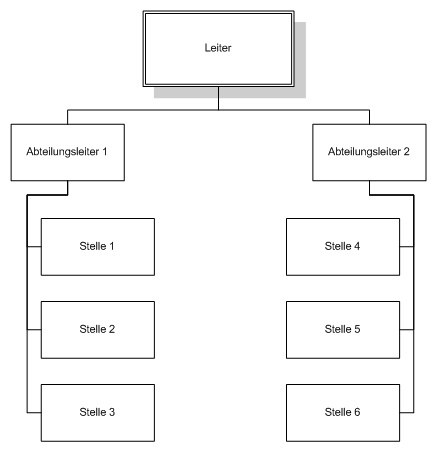
\includegraphics[keepaspectratio]{images/figure32.jpg}} \hfill{}

\caption{Abb. 3.2: Beispiel für ein Einlinienorganisation (Bernd Bosch,
CC BY-SA 3.0), Quelle:
\url{https://commons.wikimedia.org/wiki/File:Einliniensystem.jpg} (CC
Public Domain)}

\end{figure}%

\subsection{Mehrlinienorganisation}\label{mehrlinienorganisation}

Diese unterscheidet sich von der Einlinienorganisation dadurch, dass es
hier mehrere Kommunikationswege und Verbindungen zwischen den einzelnen
Organisationseinheiten gibt. In dem Beispiel von Thommen (2000) werden
drei Hierarchien bzw. Organisationsebenen dargestellt (vgl.
\hyperref[figure33]{Abb. 3.3}).

\begin{figure}

\pandocbounded{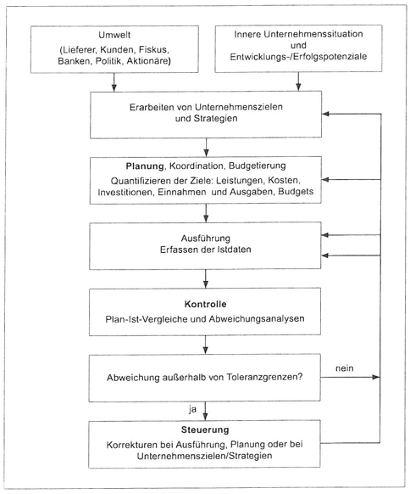
\includegraphics[keepaspectratio]{images/figure33.png}} \hfill{}

\caption{Abb. 3.3: Mehrlinienorganisation (eigene Darstellung, nach
Thommen 2000, S. 696))}

\end{figure}%

Auf der ersten Ebene ganz oben befindet sich die Unternehmensleitung,
dann gibt es eine zweite Ebene, die Abteilungen und auf der dritten
Ebene existieren die Sachbereiche bzw. die einzelnen Teileinheiten oder
vielleicht die einzelnen Häuser bei größeren sozialen Trägern. Die erste
und zweite Ebene hat eine gewisse Ähnlichkeit mit der
Einlinienorganisation. Aber es kommt noch etwas Neues hinzu, nämlich,
dass zwischen zweiter und dritter Ebene, wo letztlich alle Geschäfts-
und Managementprozesse umgesetzt werden müssen, Mehrfachzugehörigkeiten
existieren oder einfach mehrere Ansprechpartner zur Verfügung stehen.
Wenn auf der untersten, dritten Ebene z. B. Wohngruppen angesiedelt
sind, dann können die Mitarbeitenden in den Wohngruppen jeweils
gleichzeitig alle Personen auf der zweiten Ebene wie z. B. aus der
Personalabteilung, der Controllingabteilung oder möglicherweise aus dem
Einkauf und der Beschaffung ansprechen. Es gibt immer die Möglichkeit,
dass mehrere Personen für bestimmte Fragestellungen angesprochen werden
können. Ein Vorteil ist hier, dass es kurze Wege gibt und immer die
fachlichen Expert*innen angesprochen werden können und dann entsprechend
Probleme im direkten Austausch besprochen werden können, ohne eine
komplizierte Hierarchie einhalten zu müssen. Ein Nachteil ist, dass
aufgrund der Vielzahl an Kommunikationswegen oder -möglichkeiten sich
eine Organisation schnell zu einem nicht mehr überblickbaren Geschehen
entwickelt und dass die Einrichtungsleitung ggf. häufiger mit Problem-
und Konfliktfällen zu tun hat.

\subsection{Stabslinienorganisation}\label{stabslinienorganisation}

Dabei handelt es sich im engeren Sinne um eine Einlinienorganisation,
die um ein weiteres Element ergänzt worden ist, die Stabsstellen.
Stabsstellen sind solche Aufgaben- oder Funktionsbereiche innerhalb der
Einrichtung, die eine spezielle Aufgabe zur Entlastung des Vorstandes
und natürlich auch zur Verbesserung des organisationsbezogenen
Managements ausfüllen.

\begin{figure}

\pandocbounded{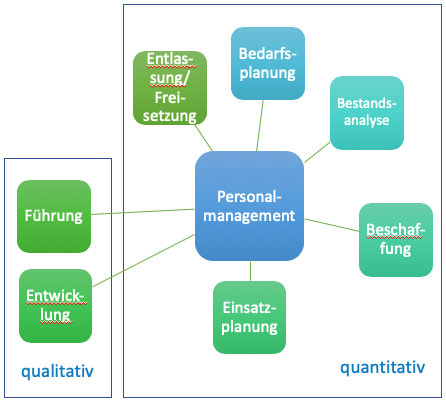
\includegraphics[keepaspectratio]{images/figure34.png}} \hfill{}

\caption{Abb. 3.4: Typische Stablinienorganisation anhand eines
Organigramm eines sozialen Trägers (nach Liedke 2017, S. 124)}

\end{figure}%

In der \hyperref[figure34]{Abb 3.4} sind beispielsweise Stabsstellen für
Personal- und Finanzwesen sowie für das Controlling und
Qualitätsmanagement zu sehen. Und darüber hinaus lassen sich natürlich
noch weitere Stabsstellen denken. Die dargestellte Einrichtung ist so
gegliedert, dass neben dem Vorstand bzw. der Geschäftsführung und den
Stabsstellen eine klassische Einlinienorganisation mit den einzelnen
Abteilungen existiert. In dem Beispiel gibt es vier Abteilungen, die
entweder Kinder- und Jugendhilfereferate oder allgemein den Bereich
Kindertagesstätten verwalten. Darüber hinaus sind verschiedene
Teilbereiche der Referate zu sehen, die nach dem jeweiligen Sachgebiet
angegliedert sind. Ein Vorteil dieser Organisationsstruktur ist, dass
die Stabsstellen genau dazu geeignet sind, den Vorstand und
Geschäftsführung zu entlasten und dass ihr Spezial- und Expertenwissen
die professionelle Arbeit der Einrichtung entsprechend zur Verfügung
steht. Nachteil dieses Organigramms könnte sein, dass sich die
Einrichtung möglicherweise sog. graue Eminenzen entwickelt, dass die
Stabsstellen über gewisses Wissen verfügen und von den einzelnen
Teilabteilungen genutzt werden kann, z. B. indem man direkt die
Controllingabteilung anfragt und der Vorstand bei bestimmten Fragen
nicht miteinbezogen wird, obwohl dies notwendig ist. So könnten sich die
Stabsstellen ihrer Kompetenz überheben, weil diese in der Regel keine
eigene Entscheidungsbefugnis besitzen, sondern „Handlungsgehilfen'' der
Unternehmensleitung darstellen.

\subsection{Matrixorganisation}\label{matrixorganisation}

Wie der Name vermuten lässt, geht es bei Matrixorganisationen um ein
Geflecht verschiedener Bereiche und Abteilungen innerhalb der
Organisation.

\begin{figure}

\pandocbounded{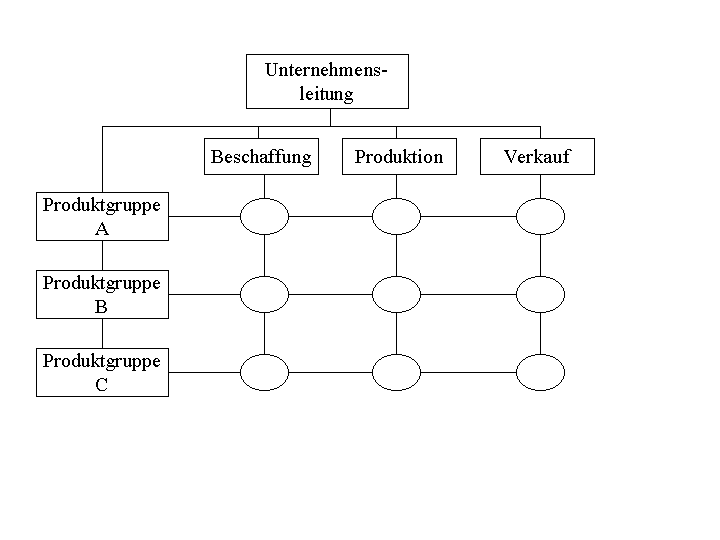
\includegraphics[keepaspectratio]{images/figure35.png}} \hfill{}

\caption{Abb. 3.5: Matrixorganisation (Wagner, 2004, \emph{Skizze einer
Matrixorganisation},
\url{https://upload.wikimedia.org/wikipedia/de/c/cb/Matrixorganisation.png}
(Public Domain))}

\end{figure}%

Die \hyperref[figure35]{Abb. 3.5} zeigt ein Unternehmen aus dem
produzierenden Gewerbe, wo verschiedene Produkte hergestellt werden. In
dem Unternehmen gibt es verschiedene Produkte, für die Manager zuständig
sind und verschiedene Verantwortliche für z. B. Einkauf, Produktion,
Verkauf (= Input-Output-Prozess). Die einzelnen Bereiche sind hier nicht
nach Funktionsbereichen untergliedert, wie dies bei den Einlinien-,
Mehrlinien- oder Stabslinienorganisation üblich ist, sondern nach dem im
jeweiligen Teilprozessverantwortlichen und Herstellungsstufen.
Anfänglich müssen Material und Bauteile beschafft werden, wobei die
Produktgruppe A beispielsweise mit der Beschaffungsabteilung den
Materialeinkauf organisiert. Wenn es dann dazu übergeht, dass das
Produkt hergestellt werden muss, ist der Produktionsmanager
Ansprechpartner. Wenn das Produkt verkauft werden soll, wird schließlich
die Marketingabteilung tätig.

Ein klarer Vorteil dieser Organisationsstruktur ist, dass die einzelnen
Bereiche sich jeweils direkt miteinander verständen können und dass
nicht noch einmal eine übergeordnete Einheit eingeschaltet werden muss.
Es steht keine Entscheidungsinstanz dazwischen; dadurch geht die
Entscheidungsfindung und auch die Umsetzung um ein Vielfaches. Ein
Nachteil ist beispielsweise, dass es hier möglicherweise auch manchmal
zu Kompetenzgerangel kommen könnte, wenn möglicherweise etwas im
Beschaffungsbereich entschieden wurde, was für den Produktionsbereich
suboptimal war und dazu geführt hat, dass ein Teil der Produktion auf
dem Schrott gelandet ist.

Die Matrixorganisation kann auch auf soziale Einrichtungen übertragen
werden. Bei den Produktgruppen könnten die verschiedenen
Leistungsbereiche oder, wenn man es als Produktgruppe übersetzt, die
Wohngruppen A, B und C stehen. Dann gibt es innerhalb der Organisation
auch noch verschiedene andere Ansprechpartner, die Leitung, die
Fachberatung oder aus anderen Bereichen wie z. B. Finanzen, Wirtschaft,
Controlling. Letztgenannte Verantwortliche können jeweils von den
einzelnen Wohngruppen direkt angesprochen werden.

\subsection{Produktgruppenorganisation}\label{produktgruppenorganisation}

Diese Organisationsstruktur stellt eine Kombination aus der Einlinien-
und Stabslinienorganisation dar (vgl. \hyperref[figure36]{Abb. 3.6}).

\begin{figure}

\pandocbounded{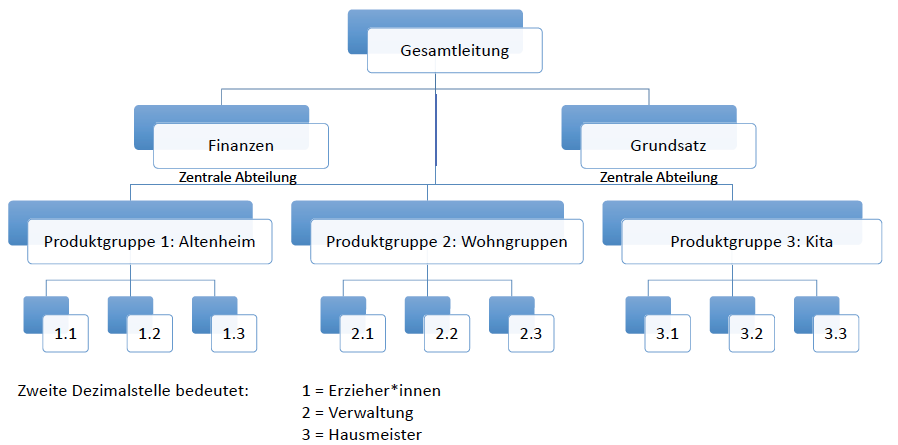
\includegraphics[keepaspectratio]{images/figure36.png}} \hfill{}

\caption{Abb. 3.6: Produktgruppen-Organisation mit zentralen Abteilungen
(nach Müller-Schöll and Priepke 1992, S. 87) zit . n. (A. Wöhrle 2012,
S. 34))}

\end{figure}%

Es gibt auf oberster Ebene die Geschäftsleitung, die verantwortlich ist
für die verschiedenen zentralen Bereiche, nämlich die Bereiche für die
Produktgruppe 1, 2, 3 usw. Die Bereichsleitung wird wiederum unterstützt
durch die Referate Finanzen und Grundsatz, um bestimmte Aufgaben zentral
abzusprechen sowie die Leitung zu unterstützen und zu entlasten. Darüber
hinaus gibt es auf der zweiten Ebene die einzelnen Produktgruppen, d.~h.
also innerhalb eines Altenheimes, Wohngruppe oder Kita gibt es
unterschiedliche (teilautonome) Teilbereiche bzw. Verantwortliche, z. B.
Heimverwaltung, angestellte Erzieher*innen und Hausmeisterdienst. Ein
Vorteil dieser Struktur ist, dass sehr stark klientenorientiert
gearbeitet werden kann. D. h. für ein Altenheim oder eine Kita gibt es
genau einen Leistungserbringer, der exakt diese Leistung und die soziale
Dienstleistung anbietet. Nachteil könnte möglicherweise sein, dass hier
die Wechselbeziehungen, nämlich das Lernen zwischen Einrichtungen eines
Trägers nicht so einfach möglich ist. Das Wissen über organisationale
Abläufe im Altenheim, in den Wohngruppen und in der Kita kann
schließlich auch zur Verbesserung der professionellen Arbeit
ausgetauscht werden.

Bisher haben wir uns mit der Aufbaustruktur beschäftigt, wobei es um die
Frage ging, wie innerhalb von Organisationen die Struktur bzw. der
formale Aufbau in Form von Organigrammen stattfinden kann.

\subsection{Reflexionsaufgabe}\label{reflexionsaufgabe}

In diesem Abschnitt ging es um die Struktur- und die Prozessperspektive
im organisationsbezogenen Management, also um die Aufbau- und
Ablaufstruktur. Die folgende Reflexionsaufgabe beschäftigt sich mit den
verschiedenen Organigrammen. Diskutieren Sie dabei die folgenden drei
Fragen:

\begin{enumerate}
\def\labelenumi{\arabic{enumi}.}
\item
  Welche Charakteristika fallen Ihnen in den einzelnen Modellen noch
  auf, die vielleicht bisher nicht erwähnt wurden?
\item
  Sehen Sie noch weitere Vor- und Nachteile, die für oder gegen diese
  Organisationsformen sprechen?
\item
  Wie meinen Sie, lassen sich die Strukturentwürfe in den sozialen
  Einrichtungen nutzen und umsetzen?
\end{enumerate}

Bisher haben wir uns mit der Aufbaustruktur beschäftigt, wobei es um die
Frage ging, wie innerhalb von Organisationen die Struktur bzw. der
formale Aufbau in Form von Organigrammen stattfinden kann.

\chapter{Prozessperspektive}\label{prozessperspektive}

\section{Phasen des
Prozessmanagements}\label{phasen-des-prozessmanagements}

Im Folgenden gehen wir zur prozessbezogenen Perspektive über. Dabei
steht die Ablauforganisation im Mittelpunkt und es stellt sich die
Frage, wie bestimmte Aufgaben innerhalb der Einrichtung strukturiert und
ggf. auch durch Verbesserungen optimiert werden können. Wir beginnen
diesen Teil jetzt mit einem Phasenmodell von Schiersmann and Thiel
(2014), die den vollständigen Ablauf des Prozessmanagements in sieben
Phasen untergliedern (vgl. \hyperref[figure37]{Abb. 3.7}).

\begin{figure}

\pandocbounded{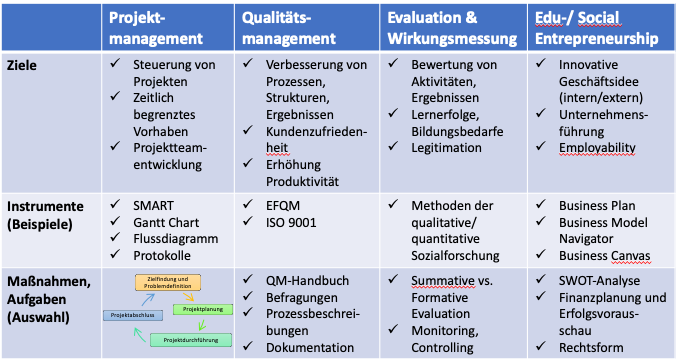
\includegraphics[keepaspectratio]{images/figure37.png}} \hfill{}

\caption{Abb. 3.7: Phasen des Prozessmanagements (nach Schiersmann and
Thiel 2014, S. 348-350)}

\end{figure}%

In der ersten Phase geht es um das Contracting, d.~h. der Kontrakt bzw.
Auftrag muss besprochen und festgelegt werden. Es muss definiert werden,
wer wie verantwortlich ist, dass ein Prozess überhaupt erst einmal
erstellt und entwickelt werden kann. Der Zeitrahmen muss definiert
werden und natürlich auch das anvisierte Ziel. In der zweiten Phase muss
festgelegt werden, wie der Prozess zukünftig gestaltet sein soll bzw.
was das Ergebnis sein soll. Im dritten Schritt müssen der Prozess bzw.
dessen Einzelbestandteile, Teilaufgaben und verantwortliche Personen
identifiziert werden. Und schließlich geht es viertens darum, den
Prozess zu modellieren. Mithilfe einer Visualisierung wird sich ein
Überblick darüber verschafft, wie die einzelnen Prozessschritte, die
Abläufe und Aufgaben sinnvoll arrangiert und verändert werden können.
Die Phase fünf setzt dann gewissermaßen diesen neu gefundenen und
entwickelten Prozess zusammen und es erfolgen Tests. In der sechsten
Phase erfolgt das Prozesscontrolling, z. B. indem das
Qualitätsmanagement die neuen Prozesse prüft, dafür Vorlagen entwickelt
und entsprechend dokumentiert. Der gesamte Prozess ist als
Controllingprozess zu verstehen. Schließlich in der siebten Phase sollen
nach diesem Modell eine Weiterentwicklung und ein Transfer angestrebt
werden, d.~h. ein Prozess ist definiert aber mit hoher
Wahrscheinlichkeit wird sich immer etwas herausstellen, was zukünftig
noch verbessert und anders umgesetzt werden kann. Daraus folgt, dass
sich um eine ständige Optimierung der Prozesse gekümmert werden muss.
Dieses 7-Phasen-Modell von Schiersmann und Thiel Schiersmann and Thiel
(2014) versucht darzustellen, wie innerhalb der Einrichtung Prozesse
gemanagt und umgesetzt werden können.

\section{4.2 Aufgabenfolgeplan bzw. Flussdiagramm
(Flowcharts)}\label{aufgabenfolgeplan-bzw-flussdiagramm-flowcharts}

Im Folgenden sollen zwei Instrumente für das Prozessmanagement innerhalb
von Einrichtungen dargestellt werden. Im Aufgabenfolgeplan bzw.
Flussdiagramm erfolgt erstens eine Visualisierung von Prozessen. Dafür
gibt es eine eigene Zeichensprache, z. B. ovale Kreise für Start- und
Endereignisse, Kästchen für Aufgabenstellungen, Pfeile für
Kommunikationswege, Rauten für Entscheidungssituationen usw. (vgl.
\hyperref[figure38]{Abb. 8}).

\begin{figure}

\pandocbounded{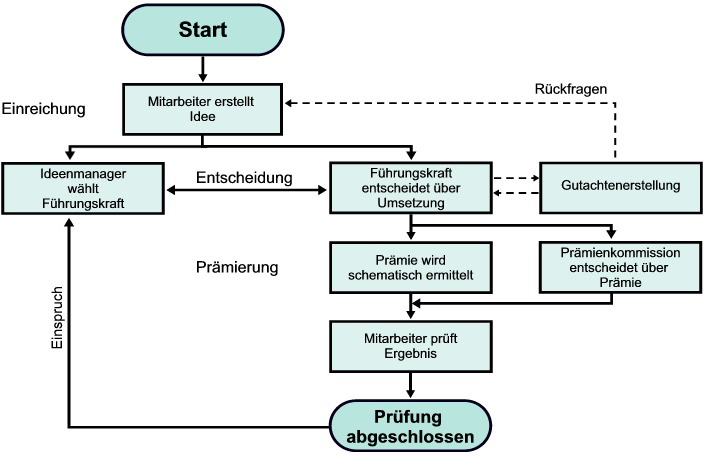
\includegraphics[keepaspectratio]{images/figure38.jpg}} \hfill{}

\caption{Abb. 3.7: Flowchart Ideenprämierung (Hagenmaier, CC-BY-SA 3.0)}

\end{figure}%

Anfangs wird eine Idee von Mitarbeitenden eingereicht, dann ist ein
Entscheidungsprozess in dem Gremium anzuregen, der zwischen Ideenmanager
und Führungskräften zu organisieren ist. Danach ist zu entscheiden, ob
eine Idee umgesetzt werden soll. Für die Entscheidung über die Umsetzung
müssen gegebenenfalls noch Gutachten von extern eingeholt werden. Falls
die vom Mitarbeiter vorgeschlagene Idee sinnvoll erscheint und umgesetzt
werden kann, kommt es zur Prämierung dieser Idee. Es gibt eine
Prämienkommission, die darüber entscheidet und diese legt dann dem
Mitarbeiter die Entscheidung über die Höhe der Prämie vor, welcher sie
im besten Fall akzeptiert. Diese Übersicht hilft dabei, den Prozess
darzustellen, wobei es allgemein gesprochen darum geht, dass eine Idee
entwickelt und prämiert wird. Ein Flussdiagramm versucht den Weg der
Entscheidungen und die Verantwortlichen, die einzubeziehen sind, zu
definieren. Es sind keine konkreten Zeitangaben gemacht worden, was ggf.
erweiterungsfähig ist.

\section{Prozesslandkarte}\label{prozesslandkarte}

Dieses zweite Instrument für das Prozessmanagement bildet, wie der Name
vermuten lässt, Prozesse in Form eines Überblicksplans, in dem die
verschiedenen Aufgaben, Verantwortlichkeiten und Schritte detailliert
dargestellt sind, ab.

\begin{figure}

\pandocbounded{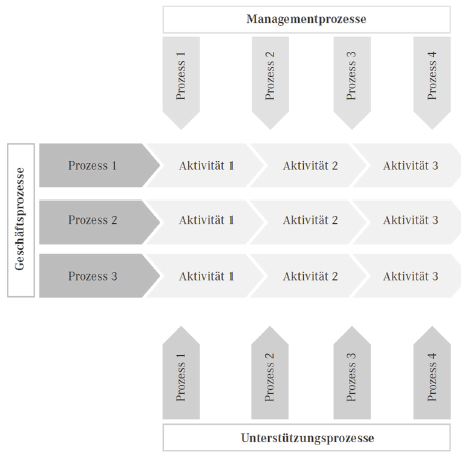
\includegraphics[keepaspectratio]{images/figure39.png}} \hfill{}

\caption{Abb. 3.9: Schema einer Prozesslandkarte (nach Liedke 2017, S.
155)}

\end{figure}%

In dem in \hyperref[figure39]{Abb. 3.9} dargestellten Beispiel gibt es
drei Bereiche, die miteinander prozessual vernetzt sind und sich
gegenseitig beeinflussen. Es können dabei drei Prozessebenen, wie z. B.
Management-, Geschäfts- und Unterstützungsprozesse unterschieden werden,
wie dies weiter oben schon anhand des St.~Galler Management-Modells
dargestellt worden ist. Zu Managementprozessen gehören z. B.
Leitungsaufgaben. Unter Geschäftsprozessen können alle Alltagsprozesse
zusammengefasst werden und bei Unterstützungsprozessen geht es darum,
dass Unterstützungsmaßnahmen wie z. B. Einkauf, Reinigung,
Hausmeisterdienste organisiert werden. In der Mitte des Schemas kann man
die einzelnen Geschäftsprozesse erkennen, die jeweils im Überblick
dargestellt werden und die einzelnen Teilaktivitäten beinhalten. Die
Teilaktivitäten werden jeweils unterstützt durch die unten dargestellten
Unterstützungsprozesse sowie durch die Managementprozesse wie z. B.
Personal, Controlling und Qualitätsmanagement.

\begin{figure}

\pandocbounded{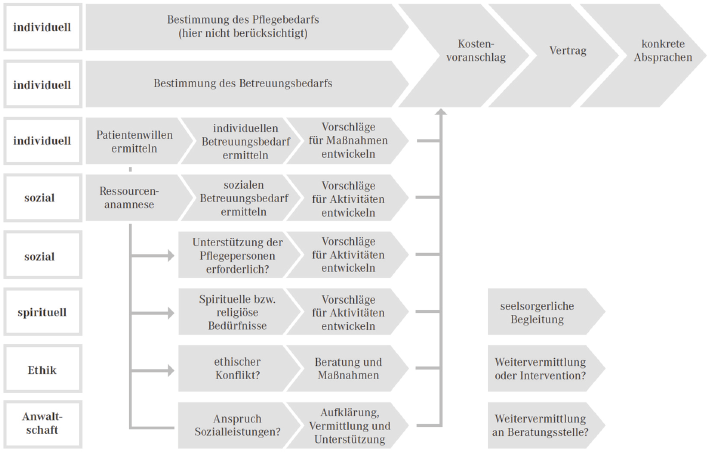
\includegraphics[keepaspectratio]{images/figure310.png}} \hfill{}

\caption{Abb. 3.10: Prozesslandkarte Erstgespräch zur Bestimmung des
Betreuungsbedarfs in ambul. Altenhilfe (nach Liedke 2017, S. 157)}

\end{figure}%

In \hyperref[n3mqgwbmxts]{Abb. 3.10} wird ein relativ komplexer Prozess,
nämlich der für das Erstgespräch zur Bestimmung des Betreuungsbedarfs in
der ambulanten Altenhilfe dargestellt. Das Beispiel ist entstanden im
Rahmen eines zurückliegenden Projekts zur Analyse diakonischer Träger in
Sachsen. In den Gesprächen, die geführt wurden, ist genau dieses Modell
aufgefallen. Dies wurde validiert und durch die jeweilige Einrichtung
abgesichert. Auf der linken Seite sind die verschiedenen Prozessebenen
dargestellt. Es gibt drei Prozessbereiche, die auf der individuellen
Entscheidungsebene relevant sind: Es gibt die soziale Ebene, wo es um
Fragen wie das Zusammenwirken mit Angehörigen oder dem Pflegepersonal
geht. Dann gibt es eine spirituelle Ebene, wo es um die Berücksichtigung
religiöser Bedürfnisse geht, und die ethische Ebene, was relevant ist
für die Qualitätssicherung und den Umgang mit Konflikten innerhalb von
Prozessen. Außerdem wird auf Ebene der Anwaltschaftlichkeit dargestellt,
was die Sozialarbeitenden bzw. die Soziale Arbeit allgemein für eine
Verantwortung trägt sowie wie und mit welchem Anspruch sie gewisse
soziale Dienstleistungen anbietet.

Grau hinterlegt sind die Teilprozesse, die der Bestimmung des Pflege-
und Betreuungsbedarfs dienen, um einen Kostenvoranschlag zu erstellen.
Auf Basis dessen kann dann der Vertrag ausgefertigt werden und es kann
zu einer konkreten vertraglichen Absprache kommen. Auf der individuellen
Ebene müssen noch weiterhin der Patientenwille bzw. der individuelle
Betreuungsbedarf beachtet und erfasst werden. Auf der sozialen Ebene
geht es darum, die verschiedenen Ressourcen, die noch für den
Betreuungsprozess zur Verfügung stehen, richtig zu koordinieren. Darüber
hinaus gilt es noch, weitere Unterstützungsmaßnahmen oder die
Unterstützung der Pflegepersonen einzuplanen, z. B. wie religiöse
Bedürfnisse durch seelsorgerliche Begleitung unterstützt werden und
ethische Konflikte gelöst werden können. Sollte eine Betreuung oder
Beratungsmaßnahmen außerhalb der Einrichtung notwendig sein, kann
entsprechend weiterverwiesen werden (z. B. Therapien, Demenzbehandlung).
Auf einer anderen individuellen Ebene geht es schließlich darum, dass
ein zusätzlicher Bedarf an Pflege festgestellt wurde, welcher zu einem
höheren Maß an benötigten Sozialleistungen führt. Wurde im Erstgespräch
nicht festgestellt, dass diese zusätzlichen Leistungen benötigt werden,
so müsste das später erneut überprüft werden.

\chapter{Organisationskultur}\label{organisationskultur}

\section{Was ist Kultur?}\label{was-ist-kultur}

Als Kultur kann man ganz allgemein ein gemeinsames geteiltes und
gelebtes Handlungs-, Orientierungs- und Symbolsystem verstehen. Damit
ist gemeint, dass es mehrere Personen gibt, die gemeinsam bestimmte
Werte, Überzeugungen und auch gewisse Handlungsweisen sowie
ritualisierte Praktiken teilen und als wichtig erachten. Darüber hinaus
verfügen Kulturen immer über bewusste und sichtbare bzw. unbewusste und
unsichtbare Elemente. Diese Unterscheidung wurde in die
Organisationskulturdebatte von Edgar Schein eingeführt und geht
letztendlich auf die Psychoanalyse zurück. Allgemein kann Kultur als
handlungsleitend verstanden werden: auf der einen Seite, sind wir durch
Kultur (z. B. Werte, Überzeugungen und Normen) geprägt, auf der anderen
Seite prägen wir auch die Kulturen, in denen wir leben. Kultur wird
nicht bewusst erlernt, sondern in einem meist längerfristigen
Sozialisationsprozess erworben bzw. angeeignet. Ein sehr bekanntes
Modell ist beispielsweise die Metapher des Eisbergs (nach Edgar Schein).
Es gibt relativ wenig Fläche bzw. Volumen eines Eisbergs oberhalb der
Wasseroberfläche. Dort sind die sichtbaren bzw. bewusst wahrnehmbaren
Aspekte von Kultur angesiedelt wie z. B. Arbeitsklima, Literatur,
Bräuche, Tänze und auch Architektur. All das stellen die wahrnehmbaren
und sichtbaren Elemente von Kultur dar. Die Sprache könnte man an der
Wasseroberfläche ansiedeln. Sprache ist für die Kommunikation und
Orientierung in der sichtbaren Welt von besonderer Bedeutung, aber auf
der anderen Seite gibt es auch unbewusste Anteile oder weniger bewusster
Anteile wie z. B. die Grammatik oder die verschiedenen Bedeutungen von
Wörtern und Sinnzusammenhängen, die man erst dann richtig verstehen
kann, wenn man sich ein Mindestmaß einer Sprache bzw. Sprachkultur
angeeignet hat. Und im unteren Bereich des Eisbergs befinden sich die
unbewussten Gedanken und Handlungskonzepte, wie z. B.
Wahrnehmungsmuster, Umgang mit Hierarchien, Machtverhältnisse,
Vorstellungen von Logik, Schönheit, Wahrheit, Erziehungsideale etc. Alle
vorgenannten Aspekte gehören zum unbewussten Teil des Eisbergs.

\section{Was ist eine
Organisationskultur?}\label{was-ist-eine-organisationskultur}

Nicht nur Individuen können Mitglieder einer Kultur sein, sondern auch
Organisationen können selbst eigene Kulturen ausbilden.
Organisationskulturen haben nach Schreyögg and Geiger (2016) in der
Regel impliziten Charakter, sie sind nicht ohne Weiteres greif- und
fassbar, sondern sie existieren im Hintergrund, sind unbewusst, nicht
explizit niedergeschrieben bzw. verschriftlicht:

Organisationkultur(en) \ldots{}

\begin{itemize}
\item
  ist ein im Wesentlichen \emph{implizites} Phänomen;
\item
  werden im Unternehmensalltag \emph{praktiziert}, gelebt und sind
  selbständig;
\item
  beziehen sich auf \emph{gemeinsame} Orientierungen, Werte etc.
  (kollektives Phänomen);
\item
  ist das Ergebnis eines \emph{Lernprozesses} im Umgang mit Problemen
  aus der Umwelt und der internen Koordination;
\item
  repräsentiert die ‚\emph{konzeptionelle Welt}' bzw. `\emph{Weltbild}'
  ihrer Mitglieder und vermittelt Sinn und Orientierung in einer
  komplexer Welt;
\item
  wird in einem \emph{Sozialisationsprozess} vermittelt und nicht
  bewusst erlernt. (Schreyögg and Geiger 2016, 177--78)
\end{itemize}

Auch wenn wir in Leitbildern versuchen, Werte, Überzeugungen und
Visionen, die Geschichte der Einrichtung niederzuschreiben, ist stets
keine vollständige Organisationsbeschreibung möglich.
Organisationskulturen entwickeln sich gewissermaßen selbstständig und
können nicht begrenzt werden durch eine Ansage der Geschäftsführung,
sondern entwickeln sich sozusagen parallel zum oder im Rahmen des
Alltags. Organisationskulturen beziehen sich auf gemeinsame
Orientierung, Werte und Überzeugungen und sind damit ein kollektives
Phänomen. So wie bereits beschrieben, geht es um das Vorhandensein
gemeinsam geteilter Werte, Überzeugungen und Symboliken. Beispielsweise
äußert sich das in der Berufskleidung, Leitbildbeschreibung und
Kommunikationsweise. Organisationskulturen sind schließlich Ergebnis
eines Lernprozesses im Umgang mit der externen und internen Umwelt; sie
sind dynamisch, entwickelt und verändern sich über den Zeitverlauf. Sie
müssen sich letztendlich immer mit der internen und externen Umwelt
auseinandersetzen. Die externe Umwelt veranlasst z. B. aufgrund von
gesetzlichen Rahmenbedingungen oder bei Veränderungen der Bedarf von
Zielgruppe Veränderungen innerhalb der Einrichtung (z. B.
Dokumentationspflicht). Konflikte, Probleme oder der Umgang mit
komplexen Herausforderungen bedingt häufig auch eine Thematisierung und
Entwicklung der Kultur innerhalb von Organisationen (z. B.
Konfliktregulierung, Aufstellen von Kommunikationsregeln). Alle
vorgenannten Aspekte können schließlich Auslöser von organisationalen
Lernprozessen sein. Schließlich repräsentiert die Organisationskultur so
etwas wie eine konzeptionelle Welt der Organisationsmitglieder, d.~h.
Organisationen wurden und werden dafür geschaffen, dass sie gemeinsame
Ziele zu verwirklichen helfen. Die Organisationskultur ist gewissermaßen
das Skript, was man im Kopf hat, wie man in der Einrichtung
zusammenarbeiten kann. Dementsprechend werden Sinn und Orientierung
innerhalb von Organisationen vermittelt und die Organisationskultur
hilft dabei, komplexe Realitäten zu bewältigen. Bestimmte
Handlungsweisen, Umgangsformen oder auch Kommunikationsregeln sind
letztlich dafür verantwortlich, dass das Miteinander bzw. die
Zusammenarbeit gelingen kann. Organisationskulturen können weder
vollständig explizit gemacht noch vollständig erlernt werden (wie z. B.
ein QM-Handbuch). Sie werden im Rahmen eines Sozialisationsprozesses
regelmäßig reflektiert und angeeignet.

\section{Modell der Organisationskultur nach Edgar
Schein}\label{modell-der-organisationskultur-nach-edgar-schein}

Im nächsten Schritt wird auf ein Modell von Edgar Schein
zurückgegriffen, der sich auf verschiedenen Kulturebenen die Frage
gestellt hat, wie Organisationskulturen aufgebaut sind. Dabei werden
drei Ebenen unterschieden, die von den sichtbaren über teilweise
sichtbare hin zu unsichtbaren Aspekten von Kulturen reichen. Auf der
sichtbaren Ebene sind die Artefakte angesiedelt, welche die
objektivierte Organisationskultur darstellen. Auf der zweiten Ebene gibt
es teilweise sichtbaren bzw. teils unbewusste Teile von
Organisationskultur, d.~h. die bekundeten Werte, die zwar
niedergeschriebene Werte und Überzeugungen darstellen. Auf der dritten
Ebene sind die unsichtbaren, meist unbewussten Anteile von
Organisationskultur, die sogenannten Grundannahmen, angesiedelt.
Dahinter verbirgt sich, wie leicht zu erkennen ist, das Konzept des
Eisbergs: die Artefakte sind direkt an der Wasseroberfläche und
sichtbar, die bekundeten Werte sind das Eisschelf, das noch ca. zwei bis
drei Meter ins Wasser sichtbar ist. Die Grundprämisse ist der Teil des
Eisbergs, der unterhalb der Wasseroberfläche ist.

Die Artefakte sind die sichtbaren Teile von Organisationen, z. B.
Strukturen und Prozesse, die nachvollziehbar, beobachtbar und aber ggf.
schwierig zu entschlüsseln sind. Dazu gehört bspw. die Sprache, die wir
verwenden. Wir setzen Sprache ein, kennen Rituale, die bestimmte
Bedeutungen haben, z. B. Tagesabläufe, Kleidung, Umgangsformen,
Kommunikationsregeln, die Fachsprache, Anreden Du oder Sie. Bei den
bekundeten Werten, auf der teilweise sichtbaren Ebene, handelt es sich
um die Strategien, Ziele und Visionen der Einrichtung, die offenkundig
und teilweise verschriftlicht sind, z. B. in Form von Leitbild,
Führungskonzeptionen oder ganz allgemein die Konzeption der Einrichtung.
Darin werden Prinzipien dargestellt, wie zusammengearbeitet werden kann
und auf welcher Basis eine professionelle Haltung existiert. Zu den
Grundannahmen gehören grundlegende Prämissen der Einrichtung, die weder
bewusst, sichtbar noch niedergeschrieben sind, z. B. das Bild vom Kind,
Weltbilder, Überzeugungen von Humanität. Dazu gehören u. a. Anschauungen
und Wahrnehmungen, Gedanken und Gefühle, die in der Einrichtung von
Bedeutung sind. Außerdem können wir uns Fragen stellen wie z. B.: Wie
pflegen wir die Beziehungen nach außen zu unserer Umwelt? Wie gehen wir
mit den Klient*innen um? Welche nicht impliziten Handlungsüberzeugungen
gibt es? Welche Überzeugung von Transparenz, Offenheit leben wir?

\section{Strategien des
Kulturwandels}\label{strategien-des-kulturwandels}

Im Folgenden werden verschiedene Strategien für den Kulturwandel
vorgestellt. Mit Kulturwandel ist gemeint, dass Organisationskulturen
nicht feststehen, sondern dass sie sich in einem kontinuierlichen
Veränderungsprozess befinden. Im vorgestellten Modell von Bate (2010;
zit n. A. Wöhrle 2001, S. 43-5) werden vier dieser Strategien
unterschieden, die aggressive, die partizipatorische, die korrosive und
die doktrinäre Strategie.

Bei der \emph{aggressiven} Strategie geht es darum, dass durch eine
entsprechende Anweisung durch die Geschäftsführung eine
Organisationskulturentwicklung ausgelöst wird. Es wird mit anderen
Worten das neue Handeln angeordnet, aufgezwungen und relativ schnell,
das ist der Vorteil, einen gewissen Impuls setzen bzw. Veränderungen
bewirken. Auf der anderen Seite, das wäre ein Nachteil, könnte daraus
auch eine Lagerbildung bzw. Pluralisierung in der Mitarbeiterschaft
erwachsen.

Auf der \emph{partizipatorischen} Ebene wird mithilfe von Team- und
Gruppenarbeit versucht, gemeinsame Ansätze zu entwickeln. Das ist
grundsätzlich der kooperative Ansatz und hier wird mehr oder weniger
danach gesucht, einen gemeinsamen Weg zu finden. Alle werden
gewissermaßen an der Problemlösung beteiligt. Vorteil davon ist, es gibt
Zusammenarbeit, Mitsprache und Teilhabe an der Entscheidungsfindung bzw.
an der Umsetzung. Ein Nachteil könnte dabei sein, dass es hier zu einem
Wandel zweiter Ordnung (siehe Organisationsentwicklung in Abschnitt 6)
kommen kann. Damit ist gemeint, dass Veränderungsprozesse als sehr
gravierend empfunden werden und es zu Brüchen kommen kann. Die
Kulturveränderung ist so tiefgreifend, dass eine komplett neue
Organisationsvision, eine neue Strategie oder/und neue Struktur für die
Einrichtung gefunden werden muss. Andererseits kann es aber auch um eine
Optimierung verschiedener (Teil-)Aufgaben, Prozesse und Strukturen
gehen.

Bei der \emph{korrosiven} Strategie wir die „politische'' Perspektive
innerhalb von Organisationen betont. Dabei wird versucht, Koalitionen zu
schmieden bzw. Netzwerke aufzubauen. Damit ist die Eröffnung von
informellen Wegen jenseits bekannter Strukturen, Verantwortlichkeiten
und Entscheidungsprozesse gemeint. Ein Vorteil ist, dass Ideen aus der
„zweiten Reihe'' ebenso kulturprägend sein können. Grundsätzlich gibt es
auch in der Sozialen Arbeit (im Sinne des Empowerments) das Prinzip,
Klient*innen stets an der Lösungsfindung zu beteiligen. Ein Nachteil
kann sein, dass es natürlich keinen Königsweg geben kann. Es könnten
sich ggf. Strukturen und Konstellationen ergeben, die zu einer
Lagerbildung und Spaltung führen und auch positive Entwicklungen
beeinträchtigen oder verhindern können.

Bei der \emph{indoktrinären} Strategie geht schließlich darum, dass man
auch auf dem Wege der Aus-, Weiter- und Fortbildung Organisationskultur
verändern kann. Vorteilhaft ist hierbei, dass relativ schnell durch eine
Wissensvermittlung eine Umorientierung stattfinden kann. Ein Nachteil
könnte sein, mit ``Umerziehungsprogrammen'' nicht immer ein
Veränderungsprozess bewirkt werden kann, da Organisationskulturen mehr
oder weniger implizit sind und diese nicht „auswendig'' gelernt werden
können.

Kurz zusammengefasst: Veränderungen können bewirkt werden durch eine
Machtausübung, wie z. B. durch Dienstanweisungen. Auf der
partizipatorischen Ebene geht es darum, Beteiligung und Teilhabe zu
ermöglichen. Auf der Ebene der informellen Netzwerke können z. B. durch
Flurfunk, Kaffeeecken oder Raucherinseln durchaus kommunikative Touch
Points beschaffen werden, wo man sich ungezwungen über neue Ideen
austauschen kann. Außerdem sind auch gezielte Weiterbildungen bzw.
Wissensvertiefungen hilfreich, wie z. B. Kennlernseminare,
Kickoff-Veranstaltung für neue Mitarbeitende, in denen Grundprinzipien,
Arbeitsweisen und die Funktionsweise der Einrichtung sowie
verantwortliche Personen innerhalb der Einrichtung vorgestellt werden.
Die vier darstellten Strategie sind nicht getrennt zu betrachten,
sondern ergänzen sich gegenseitig. Es kann auch so verstanden werden,
dass hier je nach Situation eine unterschiedliche Herangehensweise
gewählt und umgesetzt werden kann.

\section{Integrated Culture Framework nach Groysberg, Lee, Price und
Cheng
(2018)}\label{integrated-culture-framework-nach-groysberg-lee-price-und-cheng-2018}

Im Rahmen einer vor einigen Jahren erschienen empirischen Studie von
Groysberg et al. (2018a; dt. Groysberg et al. 2018b) wurde der Frage
nachgegangen, welche Bedeutung Organisationskulturen für den Erfolg von
Unternehmen haben können. Die Untersuchung beinhaltete eine Analyse der
Organisationskulturen von mehr als 230 Unternehmen in Afrika, Asien,
Europa, dem Nahen Osten, Nordamerika, Ozeanien und Südamerika, von
Führungsstilen und Werten im Rahmen von Interviews mit über 1.300
Personen in Topmanagementpositionen in Unternehmen, die sowohl
staatlich, privat als auch gemeinnützig firmiert sind, sowie einer
Online-Befragung von 25.000 Angestellten (Groysberg et al. 2018b, S.
52). Die Untersuchung förderte die folgenden acht Stile von
Organisationskulturen zutage (Groysberg et al. 2018b, S. 47-8):

\begin{itemize}
\item
  \emph{Beziehung} konzentriert sich auf Netzwerke und gegenseitiges
  Vertrauen.
\item
  \emph{Sinn} wird durch Idealismus und Altruismus verkörpert.
\item
  \emph{Lernen} ist gekennzeichnet durch Erkunden, Entfaltung und
  Kreativität.
\item
  \emph{Freude} wird durch Spaß und Begeisterung ausgedrückt.
\item
  \emph{Leistung} ist durch Ergebnisse bzw. Erfolg gekennzeichnet.
\item
  \emph{Autorität} definiert sich durch Stärke, Entschlossenheit und
  Kühnheit.
\item
  \emph{Sicherheit} definiert sich durch Planung, Vorsicht und
  Risikoabwägung.
\item
  \emph{Ordnung} ist auf Respekt, Struktur und gemeinsame Normen
  ausgerichtet.
\end{itemize}

Diese Kulturstile wurden in einem ``Integrated Culture Framework''
(\hyperref[figure311]{Abb. 3.11}) visualisiert, wobei das verwendete
4-Quadranten-Koordinatensystem auf der vertikalen Achse das
Reaktionsvermögen von Organisationsmitgliedern auf
Veränderungen\footnote{Unter Stabilität wird die Priorisierung von
  organisationaler Konsistenz, Berechenbarkeit von Entscheidungen und
  Erhaltung des Status Quo verstanden. Flexibilität betont demgegenüber
  die Anpassungsfähigkeit und Bereitschaft, Veränderungen auf- und
  anzunehmen.} (Extremwerte: Flexibiltät und Stabilität) und auf der
horizontalen Achse die zwischenmenschliche Interaktion\footnote{Bei
  Unabhängigkeit wird stärker der Schwerpunkt auf Autonomie,
  individuelle Handlungsfreiheit und Wettbewerb gelegt. Bei der
  gemeinsamen Abhängigkeit liegt hingegen die Betonung auf der
  Integration von Organisationsmitgliedern, der Gestaltung von
  Arbeitsbeziehungen und der Koordination von Gruppenaktivitäten.}
(Extrempunkte: Unabhängigkeit und gegenseitige Abhängigkeit) abträgt.

\begin{figure}

\pandocbounded{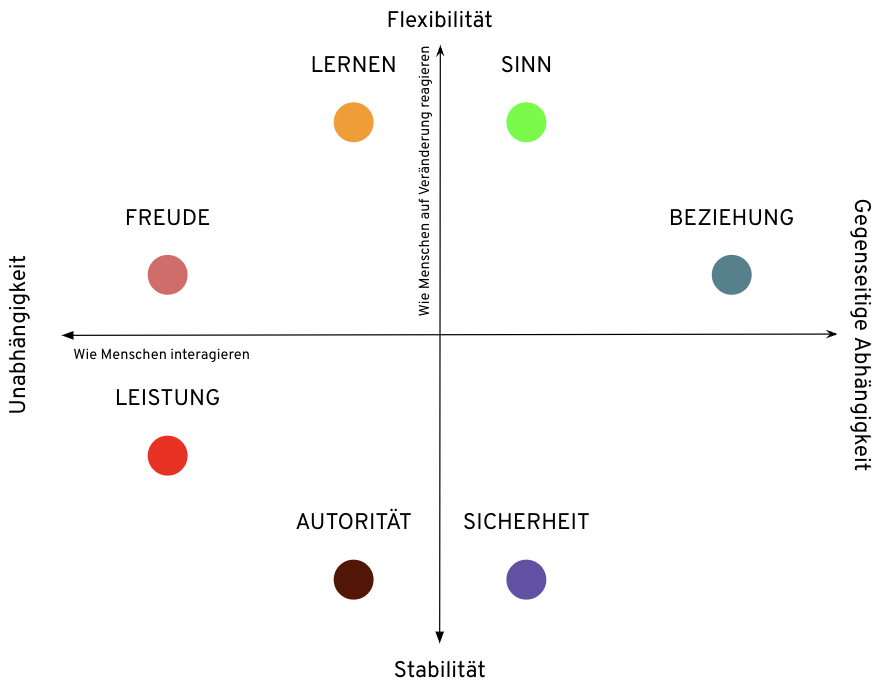
\includegraphics[keepaspectratio]{images/figure311.png}} \hfill{}

\caption{Abb. 3.11: Integrated Culture Framewor (Credits: Spencer
Stuart, In: Groysberg et al. 2018b, S. 47)}

\end{figure}%

Von den Autor:innen wird betont, dass diejenigen Kulturstile, die weit
auseinander liegen, tendentiell auch schwerer miteinander in Einklang
gebracht werden können. In der Befragung der Unternehmen wurde
festgestellt, dass insbesondere die Leistungsorientierung (89\% der
Unternehmen) und Beziehungsorientierung (63\% der Unternehmen) am
häufigsten vorzufinden sind, gefolgt von Ordnungs- und Sinnorientierung
(Groysberg et al. 2018b, S. 49).

\section{Analyse von
Organisationskulturen}\label{analyse-von-organisationskulturen}

Ein hilfreiches Werkzeug für die Entwicklung von Organisationskulturen
stellt die SWOT-Analyse (Stärken-Schwächen-Chancen-Risiken) dar. Bei den
Stärken kann grundsätzlich danach gefragt werden: Was machen wir in der
Organisation schon gut? Worauf sind wir stolz? Was motiviert uns? Und
wie sieht die aktuelle Situationslage aus? Bei den Schwächen könnten
eine Selbstüberprüfung hilfreich sein: Wo gibt es Barrieren? Welche
Konflikte, die uns immer wieder prägen, gibt es in der Einrichtung? Wo
muss eine grundsätzliche Lösung gefunden werden? Bei den Chancen geht es
um die Fragen wie: Welche Ressourcen sind vorhanden und welche müssen
vielleicht zukünftig noch weiterentwickelt werden? Wie können wir die
Kompetenzen innerhalb der Einrichtung zukünftig noch weiter ausbauen?
Dies kann z. B. durch Weiterbildungen, die Durchführung von Projekten,
oder die Kooperation mit anderen Partnern erreicht werden. Bei den
Bedrohungen und Risiken kann man sich die Frage stellen, was es denn
grundsätzlich für Schwierigkeiten und Rahmenbedingungen gibt, die wir
beachten müssen? Risiken sind negative Einflüsse, die „von außen''
kommen und die uns gewissermaßen dazu zwingen, die Organisationskultur
weiterzuentwickeln: Welche Risiken gibt es, die aktuell bestehen oder
kritische Faktoren, die sich verändern müssen? Das können bspw.
gesetzliche, wirtschaftlicher Rahmenbedingungen oder dergleichen sein.
Diese Analyse kann dabei helfen, die Organisationskultur einer
Einrichtung aus unterschiedlichen Perspektiven zu beleuchten, zu
hinterfragen und daraus Schlussfolgerungen zu ziehen.

\section{„Pflege'' von
Organisationskulturen}\label{pflege-von-organisationskulturen}

Wenn man die etymologische Begriffsentwicklung von Kultur
zurückverfolgt, so stößt man im Altertum auf einen ergologischen
(\emph{ergos}: Arbeit) Kulturbegriff. Kultur war ursprünglich mit dem
Ackerbau verbunden. Damit war das Bestellen des Ackers bzw. die Aussaat
bzw. „Pflege'' des Feldes gemeint. Dieses Prinzip kann auf die
Organisationskultur übertragen werden. D. h., dass Leistungskräfte und
auch alle Mitarbeitende die Aufgabe haben, die Organisationskultur ihrer
Einrichtung mitzugestalten. Dies ist eine Aufgabe und ein Auftrag.

Wir müssen in unseren Organisationen also ständig über Werte und
Überzeugungen sowie die Haltungen, wie wir zusammenarbeiten, was unsere
Zusammenarbeit trägt und prägt, ständig im Gespräch bleiben. Eine
lebendige Organisationskultur, wenn sie sich denn kontinuierlich
entwickelt und dabei alle Beteiligten mitnimmt, führt letztlich dazu,
alle ihre Arbeit viel motivierter, mit höherem Engagement und häufiger
auch kreativer umsetzen. Eine solche „Pflege'' der Organisationskultur
kann schließlich in verschiedener Art und Weise erfolgen: \emph{Erstens}
ist die systematische Sicht, dass Kommunikation die Organisation von
innen prägt, von immenser Bedeutung. D. h. es muss darauf geachtet
werden, dass Mitarbeitende sich nicht nur um ihre eigenen Aufgaben
kümmern, sondern sich auch für das Team verantwortlich fühlen.
Leitungskräfte stehen hierbei in der Verantwortung, regelmäßig
Möglichkeiten für Gespräche anzubieten, sodass kontinuierlich die Vision
der Einrichtung kommuniziert wird: Wo wollen wir hin? Wo stehen wir
gerade? Warum ist der nächste Schritt wichtig? Alle sind an der
Weiterentwicklung der Zusammenarbeit beteiligt bzw. zu beteiligen.

\emph{Zweitens} sollte die Organisationskultur in den Strategien,
Strukturen und Prozessen verankert werden. D. h. in der
Strategieentwicklung bzw. -erweiterung sind entsprechend Mitarbeitende
einzubeziehen, sodass alle eine Information darüber haben, was denn die
nächsten Entwicklungsschritte sind. In den Prozessen muss verankert
werden, wo es regelmäßige Zusammenkünfte und Austauschmöglichkeiten gibt
(wie z. B. Beratungen, Reflektionsmöglichkeiten, Supervision,
Konfliktlösungsangebote)?

\emph{Drittens} sollte es eine Verankerung der Organisationskultur in
der Organisation- und Personalentwicklung geben.
Organisationsentwicklung und eben auch Organisationskulturentwicklung
ist stets auch verbunden mit Personalentwicklung. Um eine
Personalentwicklung zu gewährleisten, muss das Wissen, die Kompetenzen
sowie Fähigkeiten und Fertigkeiten der Mitarbeitenden stetig
weiterentwickelt werden.

\emph{Viertens} muss stets auch neuen Mitarbeitenden in der Einrichtung
die Organisationskultur bekannt „explizit'' werden (z. B. in Kick-off
Veranstaltungen, Mentor*innen oder Coachingprogrammen zu Arbeitsbeginn).

Und schließlich \emph{fünftens} wird eine Organisationskultur in
Ritualen gefestigt, wie z. B. durch Geburtstagsrunden, kollegiale
Beratungen, Pausengestaltung, teambildende Maßnahmen. Zusammenfassend
kann gesagt werden, dass die Gestaltung von Organisationskulturen von
allen Mitgliedern der Organisation eine regelmäßige Auseinandersetzung,
Wertschätzung, Flexibilität und ein „Im-Gespräch-Bleiben'' erfordert und
verschiedene zukunftsweisende Wege und Ebenen genutzt werden müssen.

\chapter{Organisationsanalyse}\label{organisationsanalyse}

\section{Überblick zur
Organisationsanalyse}\label{berblick-zur-organisationsanalyse}

In diesem Kapitel geht es um die Organisationsanalyse als Teil der
Situationsanalyse im Unternehmen. Die Organisationsanalyse ist ein
wichtiges Instrument, das man zur Planung von Veränderungsprozessen in
der Einrichtung nutzen kann. Diese hilft beispielsweise dabei, sich
einen Überblick über die aktuelle Situation und Lage der Organisation
sowie der damit zusammenhängenden Strukturen, Prozesse und Strategien zu
verschaffen. Dabei können unterschiedliche Dinge auf dem Prüfstand
stehen: z. B. Prozessstrukturen, die Organisationskultur oder
verschiedene andere Aspekte. Im Zuge der Ausführungen wird zunächst auf
Begriff, Ziele und Vorgehensweise allgemein eingegangen. Im Anschluss
daran werden die einzelnen Phasen beschrieben und folgende Fragen
geklärt: Was muss bei der Auftragsklärung beachtet werden? Wozu dient
die Beteiligten- bzw. Stakeholderanalyse? Welche Aspekte werden bei der
Analyse der Aufbau- und Ablauforganisation sowie der Organisationskultur
untersucht? Was kann man den betriebswirtschaftlichen Kennzahlen sowie
der Kostenanalyse entnehmen? Wie kann man eine Wettbewerbsanalyse
umsetzen? Wie können schließlich Veränderungsziele formuliert werden,
die letztlich in die Organisationsentwicklung einmünden werden?
Abschließend wird ein Ausblick auf verschiedene Methoden, die man im
Rahmen der Organisationsanalyse einsetzen kann, gegeben.

\section{6.2 Was ist
Organisationsanalyse?}\label{was-ist-organisationsanalyse}

Die Organisationsanalyse kann verschiedene Zielsetzungen bzw.
Fragestellungen verfolgen. Einen guten Einblick in die Ziel- bzw.
Aufgabenstellungen der Organisationsanalyse gewährt beispielsweise die
Definition von (Kolhoff 2005, S. 6):

\begin{quote}
„Organisationsanalyse dient dazu, alle oder einzelne Systemelemente
einer sozialen Einrichtung oder eines sozialen Dienstes zu untersuchen,
um auf Veränderungen mit Verbesserungen reagieren zu können. Ziel der
Analyse ist neben -- gegenüber dem Ist-Zustand -- effizienteren und
effektiveren Aufbau- und Ablauforganisationen (technostrukturiert) auch
eine Verbesserung der Qualität der Arbeitsbedingungen der
Organisationsmitglieder (soziostrukturiert), um die Problemlösekapazität
der Organisationen zu erweitern und somit die notwendigen
Anpassungsleistungen zum Überleben auf einem zunehmend durch Konkurrenz
gekennzeichneten Markt erbringen zu können (systemstrukturiert).''
\end{quote}

Wie Kollhoff nahe legt, kann eine Organisationsanalyse auf
unterschiedlichen Ebenen stattfinden. In einer sozialen Einrichtung kann
diese entweder einzelne Aspekte oder die gesamte Organisation umfassen.
Sie dient grundsätzlich dazu, Grundlagen dafür zu schaffen, dass
organisationale Verbesserungen und Veränderungsprozesse angeregt werden.
Ziel der Analyse ist es, auf mindestens drei Ebenen aktiv zu werden: Das
ist einerseits die „Technostruktur'', welche auf die formale bzw.
administrative Struktur einer Einrichtung verweist. Damit ist
beispielsweise die Aufbau- und Ablauforganisation (also Organigramme
oder Prozessübersichten) gemeint. Verbesserungen soll es aber auch auf
anderen Ebenen geben, z. B. wo Arbeitsbedingungen der
Organisationsmitglieder geregelt werden. In letzterem Falle handelt es
sich um die „Soziostruktur''. Wie oben bereits dargestellt, sind
Organisationen soziale Gebilde. Darüber hinaus ist es möglich, dass,
wenn man Wissen über die Techno- und die Soziostruktur entwickelt hat,
zukünftig Probleme besser erkennen und lösen zu können. Mit der
Umsetzung der analysierten Veränderungsnotwendigkeiten und dem
schrittweisen Anpassungsprozess beschäftigt sich letztlich die
Organisationsentwicklung, die den Prozess umfasst, wie eine Organisation
sich den ständig veränderten Rahmenbedingungen des jeweiligen sozialen
Markts bzw. in deren internen und externen Umwelt anzupassen. Für den
Anpassungsleistungen ist beispielsweise eine Analyse der Konkurrenz-
bzw. Wettbewerbssituation im aktuellen sozialen Markt notwendig. Alle
analysierten Zusammenhänge, die die Wechselbeziehung zwischen
Organisation und der sie umgebenden Systemumwelt betreffen, wird durch
die sog. „Systemstruktur'' erfasst.

\section{Schritte der
Organisationsanalyse}\label{schritte-der-organisationsanalyse}

Um eine Organisationsanalyse durchzuführen, müssen schließlich
verschiedene Schritte geplant und umgesetzt werden, die im Folgenden
näher dargestellt werden: Im ersten Schritt der Organisationsanalyse
erfolgt die Besprechung und letztlich eine Erteilung des konkreten
Analyseauftrags und dabei sind Fragen zu klären wie: Wer ist überhaupt
dafür zuständig, wie sieht der Zeit- und Ablaufplan aus, bis hin zu der
Frage, welche Aspekte müssen in der Analyse erfasst werden. In der
zweiten Phase geht es darum, eine Beteiligten- bzw. Stakeholderanalyse
(hier werden beide Begriffe synonym verwendet) durchzuführen: D. h.,
alle Stakeholder (=Interessenbeteiligten) sind in den Analyseprozess
einzubeziehen. Am Ende dieses zweiten Schritts muss eine
Steuerungsgruppe gebildet werden. Im dritten Schritt geht es darum, die
Aufbau- und Ablaufstruktur sowie die Organisationskultur, inklusive des
Führungsverhaltens und der Mitarbeitersituation, zu untersuchen. Mit
anderen Worten geht es hier um die Techno- und Soziostruktur der
Organisation.

Im vierten Schritt geht es in der Organisationsanalyse darum, eine
Wettbewerbsanalyse bzw. Wettbewerbserkundung durchzuführen und damit die
Fragen zu klären: Wer und welche anderen Einrichtungen stehen
möglicherweise ebenfalls mit der gleichen Kundengruppen in Beziehung,
woraus entsprechende Veränderungsmaßnahmen abzuleiten sind? Die
Wettbewerbsanalyse kann man mit verschiedenen Methoden umsetzen: z. B.
Stärken-Schwächen-Chancen-Risiken-Analyse (SWOT) oder Portfolio-Analyse.
Darauf gehen wir später noch mal genauer ein. Wenn man diese ganzen
Phasen durchlaufen hat, oder Teile davon, sollte man am Ende eine Matrix
entwickeln, die verschiedene Vorschläge beinhaltet, was zukünftig in der
Organisation verändert werden muss: Welche Veränderungen sollen in
welchen Handlungsfeldern der Einrichtung umgesetzt werden?

Während wir in den Phasen 1 bis 4 den Ist-Zustand erfasst haben, geht es
abschließend im fünften Schritt darum, die Soll-Zustände zu definieren.
Der ermittelte Veränderungsbedarf ist schließlich wiederum Voraussetzung
für die zukünftige Organisationsentwicklung. Im Folgenden wird noch
einmal detaillierter auf die einzelnen Phasen eingegangen.

\subsection{Auftragsklärung}\label{auftragskluxe4rung}

Kommen wir nun im ersten Teil zu der Frage, wie die Auftragsvereinbarung
stattfindet. Man kann sich hier beispielsweise vorstellen, dass ein*e
externe*r Organisationsberater*in damit betraut werden soll, die
Organisationsanalyse durchzuführen. Ebenso lässt sich aber die
Vorgehensweise auch auf eine interne Organisationsanalyse übertragen.
Bei der Auswahl einer geeigneten Organisationsberatung müssen passende,
klar spezifizierte Vergleichsangebote eingeholt werden, die vorgelegten
Referenzen sowie die Kompetenzen der Berater*innen geprüft werden.
Besitzt die Person bereits Erfahrungen mit Einrichtung wie der unseren
bzw. der gleichen Branche. Im Auswahlprozess sollte darauf geachtet
werden, dass die Personen in der Lage sind, eine Vielzahl von Methoden
einzusetzen und entsprechende Kompetenzen mitbringen, die möglichst aus
dem gleichen Berufsfeld wie der untersuchten Einrichtung stammen. Dann
besteht eine höhere Wahrscheinlichkeit, dass die Berater*innen sich
besser in die Lage der Mitglieder der untersuchten Einrichtung zu
versetzen.

In den ersten Gesprächen mit den Verantwortlichen für die
Organisationsanalyse geht es erstens darum, einen IST-Stand zu erfassen.
Die dafür notwendigen Informationen, Zugänge zu Dokumenten und Kontakt
zu Mitarbeitenden sollte vorbereitet bzw. zur Verfügung gestellt werden,
um so eine Auftragsklärung vorzunehmen. Es geht dabei schlichtweg um die
Frage, wie ist es um die aktuelle Lage bestellt ist? Darüber hinaus
sollte auch geklärt werden, welche Methode eingesetzt wird, wie die
Grundarchitektur des Analyseprozesses aussehen kann und wie eine
Problemlösungsweg, der alle in der Beteiligung gleichermaßen
mitbeteiligt aussehen kann. Im Rahmen der Fixierung des Analyseauftrags
geht es zweitens auch darum festzulegen, welche Zielsetzungen im Rahmen
der Organisationsanalyse im Vordergrund stehen sollen: Wer ist wie
beteiligt? Wie ist der Prozess gestaltet, wie sieht der Weg der
Entscheidungsfindung bzw. Meinungsbildung aus? Es sollte von vornherein
überlegt werden, wem welche Informationen zugearbeitet werden müssen, um
nach erfolgter Organisationsanalyse den Prozess der
Organisationsentwicklung einzuleiten. Schließlich drittens sollten
schließlich die konkreten Analysemethoden festgelegt werden, um den
Prozess erfolgreich umsetzen zu können. Das sind jetzt drei ausgewählte
Dinge, natürlich keine vollständige Liste, die vereinbart werden müssen.

Schließlich muss auch die Frage geklärt werden, welche Daten und
Informationen der für die Organisationsanalyse verantwortlichen Personen
zur Verfügung gestellt werden müssen? Dabei kann es sich klassisch um
Dokumente mit betriebswirtschaftlichen Auswertungen, wie z. B.
Kennzahlen und Kostenstrukturen handeln. Hilfreich sind dabei alle
Statistiken mit Datenmaterial über das Unternehmen, das Leitbild,
Organigramm ein Überblick über das Leistungsangebot, die Zahl der
Mitarbeitenden, Evaluationen der Klient*innenzufriedenheit und
Datenmaterial zur Konkurrenzsituation (welche andere Unternehmen mit
ähnlicher Ausrichtung in der gleichen Region bzw. Stadt existieren.

Für die Strukturierung der Organisationsanalyse gibt es verschiedene
Vorschläge. Man unterscheidet einerseits in Analyseebenen und
andererseits in die Analysedimensionen. Mit den Analysedimensionen ist
der praktische Kontext der Organisationsanalyse gemeint: In welchen
Zeitraum wird was wann wie umgesetzt? Handelt es sich um eine Analyse
des gesamten Träger oder nur von Einrichtungsteilen bzw. einzelnen
Standorten?

Die Analyseebenen umfassen die verschiedenen Kriterien, auf die sich die
Organisationsanalyse beziehen soll: Beim Aufgabensystem spielen die
Arbeitsschwerpunkte und Arbeitszeiten bzw. die Arbeitskoordination
mittels entsprechender Arbeitsabläufe eine Rolle. Beim Aufgabenfeld geht
es darum, die Aufgaben, die üblicherweise in der Einrichtung anfallen,
auf den Prüfstand zu stellen. Im Rahmen der Prozessanalyse können die
Aufgabenträger eingegrenzt werden, d.~h. die zuständigen Personen in den
untersuchten Bereichen. Auf der Kommunikationsebene wäre zu fragen, wer
welche Informationen weitergeben bzw. Ansprechpartner in der
Organisation für bestimmte Aufgaben ist. Darüber hinaus kann man sich in
der Organisationsanalyse die personelle und sachliche Ausstattung der
Einrichtung genauer anschauen. Auf der Führungsebene geht es um die
Frage, wie Personalführungs- und Personalentwicklungsprozesse
ausgestaltet sind, z. B. Zielvereinbarungen, Entlohnungssystems,
Personalführungsstile, Mitarbeiterbesprechungen und
Entscheidungsfindungsprozesse. Ausschlaggebend für den Erfolg oder
Misserfolg einer Organisationsanalyse ist die Tatsache, ob die
Geschäftsleitung hinter dem Vorhaben steht oder nicht. Die Analyseebenen
und Analysedimensionen helfen dabei, den Analyseauftrag besser
einzugrenzen.

\subsection{Beteiligten- bzw.
Stakeholder-Analyse}\label{beteiligten--bzw.-stakeholder-analyse}

Im nächsten Schritt wird eine Beteiligten- bzw. Stakeholderanalyse
durchgeführt (beide Begriffe werden im Folgenden synonym verwendet).
Ziel der Analyse ist die Identifikation der Stakeholder, die im Rahmen
des Organisationsanalyseprozesses einbezogen werden sollen. Mithin
bietet diese Analyse die Möglichkeit, die oben dargestellten
Zusammenhänge der Multirationalität und Hybridität visuell darzustellen.
Eine Möglichkeit der Differenzierung unterschiedlicher Stakeholder ist
eine Tabelle, die zwischen Internen und Externen unterscheidet. Eine
andere Möglichkeit stellt ein Koordinatensystem dar, in den
unterschiedlichen Kriterien einander gegenübergstellt werden, z. B.
geografische Nähe und Distanz zu förderlichen und nicht-förderlichen
Stakeholdern. Eine hilfreiche Ressource für die Suche nach Stakeholdern
stellt das St.~Galler Management-Modell dar, in dem bereits verschiedene
Gruppen definiert wurden. Die Stakeholder-Analyse besteht aus vier
Prozessschritten.

Im ersten Schritt geht es um die Identifikation aller möglichen
beteiligten Personen und Gruppen, die mit der Organisation in Beziehung
stehen. Im zweiten Schritt geht es darum, zu definieren, wie bestimmte
Personen oder Gruppen, die ähnliche Interessen und Zielstellungen
verfolgen, zu einer Kategorie bzw. einem Cluster zusammengefasst werden
können, z. B. Leitungskräfte, Nutznießer bzw. Begünstige, Zielgruppen
bzw. Klient*innen, Finanziers, Kooperationspartner. Drittens müssen die
verschiedenen Erwartungen, Interessen, Beteiligungs- und
Einflussmöglichkeiten der einzelnen im ersten und zweiten Schritt
identifizierten Stakeholder erfasst werden. Daraus lassen sich später
die Interaktionsthemen -- wie im St.~Galler Management-Modell
dargestellt -- ableiten. Schließlich viertens kann auf Basis der
Informationen eine Steuerungsgruppe gebildet werden, die für den Prozess
der Organisationsanalyse entsprechend Verantwortung tragen wird bzw.
diesen unterstützt und berät. In der Steuerungsgruppe können
Mitarbeitende und Leitungskräfte der Einrichtung ebenso einbezogen
werden wie Externe. Die Steuerungsgruppe hat u. a. die Aufgabe, alle
notwendigen Entscheidungen für die Umsetzung der Analyse zu treffen, die
erhobenen Daten auszuwerten, zu interpretieren und zu diskutieren,
Veränderungsziele zu formulieren und den Gesamtprozess zu steuern.

\subsection{Analyse der Organisationsstruktur, -prozesse und
-kultur}\label{analyse-der-organisationsstruktur--prozesse-und--kultur}

Im nächsten Schritt wird die Ablauf- und Aufbaustruktur der Einrichtung
analysiert. Angeknüpft werden kann hierbei einerseits an die
verschiedenen Organigramme, z. B. (Stabs-)Linien, Produkt- und
Matrixstruktur, die eine Organisation dabei unterstützen,
Verantwortlichkeiten und Aufgabenbereiche zu definieren. Darüber hinaus
sind auch Stellen- bzw. Tätigkeitsfeldbeschreibungen hilfreich, um
daraus Informationen über die Unter-/ Überordnung von Aufgabenfeldern zu
gewinnen. Im Rahmen der Analyse der Ablauforganisation geht es um die
Frage, welche Mitarbeitende wie organisatorisch eingebunden sind und
welche Dokumentations- und Kommunikationswege existieren.

Hilfreiche Analyseinstrumente stellen dabei beispielsweise Zeit- und
Dienstpläne dar. Gesetzt der Fall, in einer Einrichtung soll die
Notwendigkeit einer Fremdunterbringung geprüft werden, so kann man einen
Zeit- und Ressourcenplan sowie die Entscheidungswege darstellen, um
damit den IST-Stand des Prozesses darzustellen, woraus später
Veränderungsmaßnahmen abgeleitet werden sollen. Mithilfe eines solchen
Plans kann die Ablauf- und Aufbaustruktur visualisiert werden. Im
besagten Beispiel muss dargestellt werden, wie der Prozess von der
Anfrage zur Überprüfung im ersten Schritt über verschiedene Vermerke,
die in den einzelnen Fachbereichen bzw. Sachgebieten geprüft und
weitergereicht werden, bis zur endgültigen Entscheidung und dem Bericht
über die Notwendigkeit oder Ablehnung einer Fremdunterbringung gestaltet
ist, wie viele Zeit- und finanzielle Ressourcen dabei verbraucht werden.
Ein solcher Ablaufplan gibt einen klaren Überblick darüber, wer was in
welchem Sachgebiet mit welchen Ressourcen umsetzt. Auf Basis der Analyse
kann schließlich überlegt werden, welche Veränderungs- bzw.
Gestaltungsmöglichkeiten bestehen, um den Prozess ggf. ein wenig zu
vereinfachen, ohne damit professionelle Entscheidungskompetenz damit zu
gefährden.

Weiterhin kann man neben der Ablauf- und Aufbaustruktur, also der
Technostruktur einer Organisation, auch die Soziostruktur betrachten.
Dabei geht es um Fragen wie z. B.: Wie sehen die Arbeitsbedingungen aus,
welche Maßnahmen der Personalentwicklung gibt es. Im Rahmen der
systemischen bzw. systematischen Organisationsanalyse beschäftigt man
sich mit der Frage, welche Kommunikationsprozesse, Führungsstrukturen in
der Einrichtung existieren und auf welche Art und Weise Entscheidungen
überhaupt getroffen werden. Diese Informationen sind wichtig, um später
die Beziehungs- bzw. Interaktionsprozesse in Organisationen zu
untersuchen.

Viele Organisationsberatungsansätze beschäftigen sich mit der
Soziostruktur sowie den psychodynamischen Prozessen. Beispielsweise
werden in allen Organisationen sogenannte Spiel gespielt, die mitunter
zuträglich sein können aber überwiegend negative Effekte haben. Damit
sind keine Kartenspiele oder dergleichen gemeint, sondern Menschen
spielen miteinander in Organisationen um Ressourcen, Macht, Anerkennung
etc. Die bekanntesten Beispiele sind wohl die sog. Machtspiele, z. B.
wenn gegen ein Vorhaben bewusst Widerstandes geleistet wird, sich eine
Gruppe Mitarbeitender gegen eine Entscheidung auflehnt und nicht gewillt
ist, bestimmte Veränderungsmaßnahmen umzusetzen bzw. zu unterstützen.
Mit anderen Worten handelt es sich dabei um Widerstandsspiele. Darüber
hinaus gibt es auch Machtaufbauspiele, wo es darum geht, dass einzelne
Person in einer über besonderes (Experten-)Wissen verfügen. Manchmal
entwickeln sich Strukturen in der Einrichtung, wo für eine Beratung
nicht die Person gefragt wird, die formal gesehen dafür zuständig ist,
sondern eben die Person, die am besten darüber Bescheid weiß.
Erfahrungswissen und Funktion müssen nicht immer zusammenfallen. Ebenso
können sich in Einrichtungen Allianzen bilden, also Gruppen, die sich
sozusagen gemeinschaftlich für Ideen einsetzen. Weiterhin gibt es
Bekämpfungsspiele, in denen Entscheider*innen mit Experten, die sich in
einem Tätigkeitsfeld besonders gut auskennen in Verhandlung stehen,
diskutieren und aushandeln müssen. Schließlich gibt es
Veränderungsspiele, wenn Personen aufgrund von Insider- oder Vorwissen
über mehr Informationen verfügen und sich dadurch Vorteile gegenüber
Personen, die diese Informationen nicht haben, verschaffen. Das lässt
sich häufig in Verhandlungen zwischen Einrichtungsleitung,
Mitarbeitenden und Personalrat oder in politischen Gremien verfolgen.
Mit anderen Worten führen viele dieser Spiele dazu, dass die formale
Organisationstruktur und Organisationskultur unterwandert wird. Diese
Ausführungen sollen kein schlechtes Licht auf Organisationen richten,
vielmehr ist dies als eine Beschreibung der Realität zu analysieren und
zu verstehen. Eine andere Frage ist, wie man damit umgeht und die
Organisationskultur (um-/weiter-)gestaltet. Grundsätzlich gibt es bei
allen diesen Formen von Organisationsspielen auch positive Aspekte. Z.
B. kann eine Allianz dazu führen, dass eine wichtige Entscheidung
getroffen wird. Was allerdings problematisch ist, ist wenn Informationen
bewusst zurückgehalten werden damit die Transparenz gefährdet ist bzw.
kein Fairplay mehr stattfindet

Ebenso kann im Rahmen dieses Analyseschritts das Mitarbeiterverhalten,
mit anderen Worten das Zusammenspiel zwischen Mitarbeitenden und
Leistungskraft, untersucht werden: z. B. Beteiligungsmöglichkeiten an
der Strategie- bzw. Leitbildentwicklung, unterschiedliche Auslastungen
und Belastungen einzelner Mitarbeitenden, notwendige
Personalentwicklungsmaßnahmen zur Weiterqualifikationen des Personals,
Unterstützung intrinsischer Motivation der Mitarbeitenden. Darüber
hinaus spielt auch die Organisationskultur eine Rolle. So könnte man
fragen, welche ritualisierten gemeinsamen Feste und (wie oben erwähnt)
bestimmte Fördermöglichkeiten es gibt. Darüber hinaus gilt es Gründe für
ständige Fluktuationen zu finden bzw. Aktivitäten des Arbeitgebers zur
Mitarbeiterbindung ausfindig zu machen. Schließlich sollte auch
analysiert werden, welche Maßnahmen zur Verbesserung bzw. Entwicklung
der Arbeitsbedingungen bzw. des Arbeitsplatzes zur Verfügung stehen.
Ebenso steht bei der Untersuchung des Mitarbeiterverhaltens die Frage
der Personalführung im Mittelpunkt: z. B. welche Führungsansätze werden
gelebt, autoritäre bzw. autoritative, demokratisch geprägt. Aus allen
diesen Aspekten lässt sich am Ende des Analyseprozesses ein
Veränderungsbedarf ableiten.

\subsection{Kostenanalyse}\label{kostenanalyse}

Im Rahmen der Kostenanalyse werden die Informationen und Daten des
Rechnungswesens und Controllings analysiert. Dabei geht es darum,
herauszufiltern, welche Tätigkeiten denn welche Kosten aufwerfen. Es
geht auch darum, Kostentreiber zu identifizieren und Ursachen für
ineffizienten Veränderungen in der Kostenstruktur aufzudecken, z. B.
wenn die fixen Kosten durch ungünstige Verträge gestiegen sind, zu hohe
Sozialleistungen anfallen, die möglicherweise auf einen hohen
Krankenstand zurückzuführen sind. Ineffizienzen in der
Organisationsstruktur und in den Abläufen kann man in der Regel auch in
der Kostenstruktur der Einrichtung nachvollziehen. Als Datenquellen kann
man zum Beispiel Betriebsabrechnungsbögen und
Wirtschaftlichkeitsabrechnungen verwenden, um herauszufinden, wo welche
kosten und wofür anfallen. Hintergrund der Kostenanalyse ist es weniger,
einfach blind Rationalisierungsmaßnahmen zu entscheiden, sondern die
Ursachen für Veränderungen zu identifizieren. Dies ist stets mit der
Frage verbunden: Wo können wir in unserer Einrichtung noch besser
werden, um damit besser unsere Aufgaben- und Zielstellung bzw.
Einrichtungszweck zu erfüllen?

\subsection{Wettbewerbs- bzw.
Konkurrenz-Analyse}\label{wettbewerbs--bzw.-konkurrenz-analyse}

Im Rahmen der Wettbewerbs- bzw. Konkurrenz-Analyse werden vier
Instrumente eingesetzt, die im Folgenden kurz erläutert werden sollen.
\emph{Erstens} gibt es die sogenannte Potenzialanalyse, bei der die
unternehmensinternen Kompetenzen, wie z. B. die Qualifikation des
Personals, Finanzen und Kostenstruktur analysiert werden (vgl. alle
vorherigen Schritte der Organisationsanalyse). Mit anderen Worten werden
die eigenen Ressourcen, die Aufgabenbereiche und Strategien dargestellt.
\emph{Zweitens} gibt es die Konkurrenzanalyse: Dabei fragen wir danach,
welche Zielgruppen eigentlich von den Einrichtungen bedient werden, wie
man diese mit anderen Einrichtungen der gleichen Region, der gleichen
Stadt oder des gleichen sozialen Marktes vergleichen kann. Außerdem wird
danach gefragt, ob sich bestimmte Bedarfe verändert haben, oder ob es
Hinweise darauf gibt, ob sich die Struktur des Klientels verändert hat.
\emph{Drittens} kann eine Stärken-Schwächen-Analyse durchführt werden,
mit deren Hilfe nach dem Innen des Unternehmens geschaut wird. Dies kann
durch Einsatz eines Fragebogens geschehen oder im Rahmen eines
Workshops, im dem die Ressourcen, wirtschaftliche Situation,
Personalbestand etc. erfasst und dokumentiert wird. \emph{Viertens} gibt
es die Portfolio-Analyse. Dabei geht es darum, dass nicht nur die Innen-
und Außensicht aufgenommen wird. Dabei steht die Frage im Vordergrund,
wie wir mit unseren Dienstleistungen im jeweiligen sozialen Markt
positioniert sind. Die Idee zur Portfolio-Analyse kommt aus den
Finanzwissenschaften: Portfolio heißt, dass wir so eine Art Warenkorb
haben, indem wir unterschiedliche Geschäftsfelder zusammengefasst sind
(z. B. Altenheim, Jugendhilfeeinrichtung, Wohngruppen,
Kindertageseinrichtung). Jede dieser Einrichtungen eines Trägers trägt
in unterschiedlicher Weise zur Entwicklung der Einrichtung bei. Diese
Methode verschafft damit einen Überblick über die verschiedenen
Geschäftsfelder und visualisiert, welche Position unsere Einrichtung im
Wettbewerb besitzt. Ein Vergleich mit anderen Einrichtungen ermöglicht
die Herausarbeitung des sog. USP (Unique Selling Proposition) bzw. von
Alleinstellungsmerkmalen oder Kernkompetenzen.

\subsection{Erarbeitung von Soll-Vorschlägen für
Handlungsfeldveränderungen}\label{erarbeitung-von-soll-vorschluxe4gen-fuxfcr-handlungsfeldveruxe4nderungen}

Im letzten Schritt der Organisationsanalyse findet die Zielbestimmung
statt. Nachdem nun in den vorherigen Phasen der aktuelle IST-Zustand
ermittelt wurde, muss in diesem letzten Schritt der gewünschte
Sollzustand bzw. die Ziele für die umzusetzenden Veränderungen
beschrieben werden. Dies kann in zwei Schritten erfolgen, erstens in
Gestalt des \emph{Ursache-Problem-Wirkungsbaums} oder zweitens durch
eines \emph{Reframings im Handlungsmöglichkeiten-Ziel-Wirkungsbaum}.

Im \emph{Ursache-Problem-Wirkungsbaum} geht es darum, ausgehend von den
Wirkungen, das dahinterliegende Kernproblem zu identifizieren, warum
bestimmte Abläufe oder Strukturen ineffizient sind. Aus dem Kernproblem
lassen sich dann verschiedene Ursachen ableiten, die verantwortlich
dafür gewesen sind, dass Probleme aufgetreten sind. Mit anderen Worten
handelt es sich um eine dreischichtige Problemanalyse, die im Folgenden
anhand eines Beispiels beschrieben werden soll. Es wurde festgestellt,
dass in die Arbeit des Jugendamts ein Vertrauensverlust entstanden ist,
was daran abgelesen werden kann, dass Klient*innen das Jugendamt meiden
und sich „allein gelassen'' fühlen. Wenn man danach fragt, was dabei das
eigentliche Kernproblem darstellt, kann relativ schnell erfasst werden,
dass die Klient*innen unzufrieden sind mit den Leistungen des
Jugendamts. Ursachen für diese Unzufriedenheit sind bspw. lange
Wartezeiten, unfreundliche Mitarbeitende und unzureichende Beratung. Aus
diesen Ursachen lässt sich die Unzufriedenheit der Klient*innen
schließen. Wenn wir weiter fragen, wie die Unfreundlichkeit der
Mitarbeitenden erklärt werden kann, lässt sich das darauf zurückführen,
dass dieser aktuelle Zustand im Jugendamt möglicherweise auf die
fehlende Motivation der Mitarbeitenden aufgrund ihrer geringe
Eigenverantwortlichkeit (Sozialstruktur) sowie lange, bürokratische Wege
(Technostruktur) zurückzuführen ist.

Mithilfe des \emph{Reframing-Ansatzes} gehen wir von der veränderten
Wirkungsbeschreibung über die neue Zielstellung hin zu den zu planenden
Interventionsmöglichkeiten und einzusetzenden Ressourcen. Damit wird
gewissermaßen das vorherige Bild noch einmal umgekehrt. Durch die neuen
Handlungsmöglichkeiten wird dann eine andere Wirkung erzielt. Dies sei
wieder anhand eines Beispiels erläutert: Zunächst muss die veränderte
Wirkung bzw. der Sollzustand definiert werden. Wir wollen erreichen,
dass zukünftig eine vertrauensvolle Zusammenarbeit mit den Klient*innen
ermöglicht wird. Das kann letztlich nur gelingen, wenn diese das
Jugendamt „angstfrei'' aufsuchen können und das Amt als „Partner'' und
weniger als eine (Verwaltung-)Behörde betrachten. Um diese gewünschte
Wirkung zu erzielen, muss bei allen Prozessen und Maßnahmen darauf
geachtet werden, dass die Zufriedenheit der Klient*innen gesteigert wird
(Zielebene). Das Amt entscheidet nicht über die Klient*innen hinweg,
sondern das Verhältnis wird als Co-Konstruktion von sozialer
Wirklichkeit verstanden. Um dieses Ziel umzusetzen, bedarf es
schließlich einer zügigen Bearbeitung der einzelnen Anträge, eines
freundlichen Gegenübertretens und einer umfassenden Beratung.
Freundliche und motivierte Mitarbeitende wird es nur dann geben, wenn
diese durch mehr Eigenverantwortung ausgestattet werden und es kurze,
überschaubare Verwaltungswege gibt.

\section{Methoden der
Organisationsanalyse}\label{methoden-der-organisationsanalyse}

Hinsichtlich der Auswahl geeigneter Methoden für die
Organisationsanalyse ist zunächst auf die Analysedimensionen und die
verschiedenen Ansätze im Rahmen der empirischen Sozialforschungsmethoden
einzugehen. Hinsichtlich der \emph{Analysedimensionen} sind insbesondere
die Struktur-, Prozess- und Ergebnisqualität von Belang. Im Kontext der
Strukturqualität stellt sich die Frage, inwieweit die Aufbau- bzw.
Organisationsstruktur der Einrichtung umgesetzt wird. Bei der
Prozessqualität stehen die Abläufe innerhalb der Institution im
Vordergrund. Und bei der Ergebnisqualität untersuchen wir, wer wann wie
in der Einrichtung tätig ist bzw. zum Erfolg der Einrichtung beigetragen
hat. Hierbei ist außerdem zu fragen, welche Kriterien angelegt werden
können, um den Erfolg zu messen.

Hinsichtlich der verschiedenen \emph{Sozialforschungsmethoden} ist
zunächst zu fragen, welche Untersuchungsperspektive einzunehmen ist:
entweder qualitativ-orientierte Verfahren, die stärker auf eine
Exploration, Hypothesenbildung, Einzelfallanalyse, Untersuchung sozialer
Repräsentationen und Sinnzusammenhänge abzielen, oder umgekehrt im Sinne
quantitativer Sozialforschung, die auf eine Überprüfung von
theoretischen Zusammenhängen und Hypothesenüberprüfung abzielen. Je
nachdem könnten dann Befragungen und Experimente (stärker quantitativ)
oder Beobachtungen und Inhaltsanalyse (stärker qualitativ) eingesetzt
werden. Je nachdem welches verfahren wir wählen oder welchen Weg wir
gehen, sind auch bestimmte Methoden besser geeignet. Kurz
zusammengefasst geht es sozusagen bei der qualitativ-orientierten
Methodik um Hypothesenbildung und bei der quantitativ-orientierten
Methodik um eine Hypothesenüberprüfung.

Wie bereits festgestellt, gibt es eine große Bandbreite von Methoden,
die in der Organisationsanalyse eingesetzt werden können. Im Rahmen der
\emph{quantitativen Ansätze} können z. B. Aktenanalysen, Erhebungsbögen,
Vermerke, Verfügungen, Berichte, Gutachten, Briefe eingesetzt werden, um
dokumentierte Prozesse innerhalb der Einrichtung nachvollziehen zu
können. Mithin eigenen sich dabei auch die verschiedenen Dokumente des
Qualitätsmanagements. Dabei können unterschiedliche Foki eingenommen
werden: Bei der Frequenzanalyse wird nach der Häufigkeit und Intensität
bestimmter festgestellter Beobachtungen gefragt (z. B. Häufigkeit
bestimmte Fälle, Entscheidungen) oder im Sinne einer ABC-Analyse nach
Gewichtungen und Priorisierungen gefragt (z. B. wie hoch ist die
Relevanz und Priorität bestimmter Fälle, während A die höchste und C die
niedrigste Priorität besitzt). Bei Valenzanalysen wird versucht, die
Wichtigkeit zu bewerten. Valenz heißt, dass wir uns mit dem Wert
beschäftigen, etwas bewerten wollen (wie z. B. Mitarbeiterbefragungen).
Bei der Kontingenzanalyse werden Zusammenhänge untersucht bzw. die
Verbindung zwischen Elementen versucht herzustellen, um damit nach
Ursachen zu fragen und Wirkungen besser beurteilen zu können. Dabei
können beispielsweise Beschreibungen und Erklärungen von Akteninhalten
und Dokumenten gesucht werden, die uns in die Lage versehen,
Zusammenhänge zu erkennen.

Mit Hilfe der \emph{qualitativen Verfahren} geht es dann darum,
Einzelpersonen oder Gruppen zu befragen und an deren Sichtweisen und
Expertisen anzuknüpfen. Dazu sind bspw. mündliche Befragungen geeignet,
wie z. B. Individualinterviews, Gruppendiskussionen. Es lassen sich aber
auch schriftliche Befragung (z. B. per E-Mail oder Fragebogen)
einsetzen, allerdings nicht im Sinne eines strukturierten Fragebogens,
sondern mit möglichst offenen Fragen, die einen breiten Antwortraum
ermöglichen. Außerdem können Beobachtungen durchgeführt werden und auch
Tagesberichte analysiert werden, um damit Aufschluss zu bekommen für
über die verschiedenen Abläufe und Tätigkeiten, die eine Person oder
mehrere Personen während des Tages ausüben. Das ist eine wertvolle
Methode für Arbeitsanalyse z. B. im Rahmen von Abschlussarbeiten. Bei
der Tagesberichterfassung wird eine strukturierte Beobachtung
durchgeführt, in dem Daten der Gesprächsperson (Name, Abteilung, Raum,
Datum, Kontaktdaten) und für alle (Teil-)Aufgaben während des Tages die
jeweils benötigte Zeit (in Minuten/Sekunden), Arbeitsmittel,
Ansprechpartner, Einzeltätigkeit, Besprechung oder Zusammenarbeit
differenziert erfasst werden. Damit ist es möglich, ein genaueres Bild
von den tatsächlichen Arbeitsabläufen, Interaktionen und Arbeitsinhalten
während des Alltags zu erhalten. Diese Erkenntnisse können dann einen
Ausgangspunkt für Prozess- und Strukturanalyse, aber für die
Organisationskultur darstellen.

\chapter{Organisationsentwicklung}\label{organisationsentwicklung}

\section{Was ist
Organisationsentwicklung?}\label{was-ist-organisationsentwicklung}

In diesem Abschnitt beschäftigen wir uns mit der
Organisationsentwicklung. Was fällt Ihnen zu der Fragestellung: „Was ist
Organisationsentwicklung?'' ein. Bitte überlegen Sie kurz und notieren
Ihre Ideen.

Bei der Auseinandersetzung mit dem Begriff „Organisationsentwicklung''
soll uns folgende Definition der Gesellschaft für
Organisationsentwicklung behilflich sein:

\begin{quote}
„Organisationsentwicklung kann man allgemein als einen längerfristigen
angelegten Entwicklungs- und Veränderungsprozess von Organisationen
verstehen, der in nun tätigen Mitarbeitenden und Menschen. Der Prozess
beruht auf Lernen aller Betroffenen durch direkte Mitwirkung und
praktische Erfahrung. Sein Ziel besteht in der gleichzeitigen
Verbesserung der Leistungsfähigkeit der Organisation (Effektivität) und
der Qualität des Arbeitslebens (Humanität)'' (Gesellschaft für
Organisationsentwicklung zit. in Kolhoff 2009).
\end{quote}

Was können wir aus dieser längeren Definition herausarbeiten?
Grundsätzlich kann man sagen, dass Organisationsentwicklung einen
längerfristigen Prozess darstellt:

\begin{itemize}
\item
  wie verändern sich Einrichtungen,
\item
  Entwicklungs- und Veränderungsprozess von Organisationen sowie
\item
  Ermittlung von notwendigen, zukünftigen Veränderungen.
\end{itemize}

Es sind nicht nur Strukturprozesse innerhalb der Organisation die sich
verändern, sondern es muss auch auf der Ebene der Mitarbeitenden
mitgedacht werden, wie der Veränderungsprozess umgesetzt werden kann. D.
h., Hintergrund der Organisationsentwicklung ist, den Prozess der
Veränderung in Organisationen sowie im Verhalten und der Einstellung von
Mitarbeitenden herauszufinden. Der Prozess der Veränderung bedeutet für
alle Betroffenen, dass diese die Veränderung mit umsetzen und für sich
verbindlich erklären müssen. Dies sollte durch Mitwirkung geschehen und
es sollten selbstverständlich auch praktische Erfahrungen mit einfließen
dürfen. In Ergänzung zu o. g. Definition gibt es verschiedene
theoretische und praktische Modelle, die man nutzen kann, um eine
Organisationsentwicklung umsetzen zu können (wie z. B. das
Dreiphasen-Modell von Kur Lewin; siehe Abschnitt 1.2.4. Im letzten Satz
der Definition ist noch etwas zur Zielsetzung ausgesagt: Warum tun wir
das? Wir wollen etwas verbessern, wir wollen die Zusammenarbeit
innerhalb der Organisation verändern, was dazu führt, dass wir hinterher
besser unseren Aufgaben gerecht werden können. Hier wird von
Leistungsfähigkeit der Organisation und Effektivität gesprochen, d.~h.,
wir müssen die Organisationsentwicklung auch in dieser Richtung
verstehen: Wir versuchen, unsere Ziele, unsere Strategien und die
Organisationskultur, unsere Prozesse und Strukturen zu optimieren bzw.
an unseren jeweiligen Leistungsauftrag anzupassen. Letztendlich geht es
auch um die Qualität des Arbeitslebens bzw. des Zusammenarbeitens. Wir
versuchen Organisationsentwicklung auch deswegen einzusetzen, weil sich
unsere Einrichtung und wir uns als Mitarbeitende ganz allgemein
innerhalb dieser Einrichtung weiterentwickeln wollen.

\section{Erfolgsfaktoren im Rahmen der
Organisationsentwicklung}\label{erfolgsfaktoren-im-rahmen-der-organisationsentwicklung}

Man kann sich fragen, wie solche Organisationsentwicklungen erfolgreich
sein können oder werden. Es gibt verschiedene Untersuchungen, die zu
ähnlichen Ergebnissen bei der Fragestellung gekommen sind, woran die
Erfolgsfaktoren festgemacht werden können und ob eine
Organisationsentwicklung zu dem gewünschten Ziel geführt hat. In den
Untersuchungen wurden verschiedene Aspekte genannt, die Aussage dazu
treffen, dass z. B. Barrieren und Grenzen zwischen den Mitarbeitenden
überwunden werden, dass Betroffene einbezogen werden sollen, dass
konsequent an der Problemlösung gearbeitet werden muss und dass man
Kenntnis über die Zusammenhänge der jeweiligen Veränderungsprozesse
haben soll. Des Weiteren ist dabei die Bedeutung der Kommunikation für
den Prozess der Veränderung noch einmal hervorgehoben und letztendlich
auch die aktive Unterstützung des Topmanagements, also der Leitung des
Trägers. Auch werden verschiedene Einfluss- und Erfolgsfaktoren
deutlich, die dazu führen, dass wir mit der Organisationsentwicklung zu
unserem Ziel kommen. Es sind grundsätzlich personalrelevante oder
personenrelevante Informationen (vgl. A. Wöhrle 2012, S. 24)
(\hyperref[figure312]{Abb. 3.12}). Es sind sozusagen die Mitarbeitenden
und die Mitglieder von Organisationen selbst, die beteiligt werden
müssen und die offen kommunizieren sowie mit einbezogen werden müssen,
damit die Organisationsentwicklung gelingt. D. h., der „Faktor Mensch''
ist hier von besonderer Bedeutung für den Erfolg.

\begin{figure}

\pandocbounded{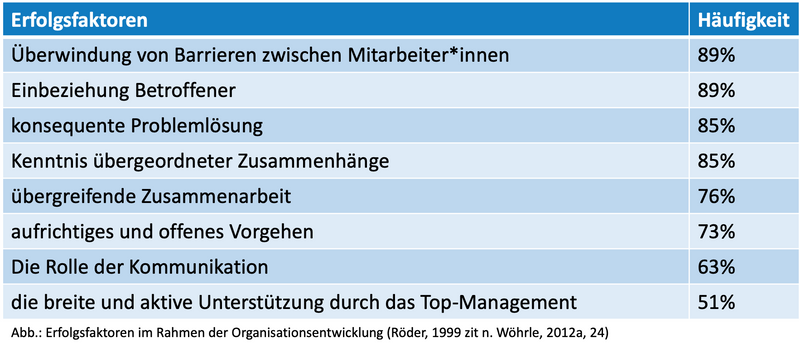
\includegraphics[keepaspectratio]{images/figure312.png}} \hfill{}

\caption{Abb. 3.12: Erfolgsfaktoren im Rahmen der
Organisationsentwicklung (Röder 1999, zit. n. A. Wöhrle 2012, S. 24)}

\end{figure}%

Es gibt verschiedene Studien, die versuchen zu belegen, dass der
Großteil von Organisationsentwicklungsprozessen in der Regel schief
gehen, d.~h., dass man nicht die Ziele erreicht, die man hätte erreichen
wollen. Auch wenn es schwierig ist, dies methodisch festzustellen, geht
man davon aus, dass man nur bei einem kleinen Prozentsatz - einige sagen
30 oder gar 40 \% der Fälle - von einem Erfolg in der
Organisationsentwicklung im eigentlichen Sinne ausgehen kann. Die
bedeutet, dass sich die Schere für den tatsächlichen Erfolg am Ende des
Entwicklungsprozesses zwischen 30 \% und 70 \% bzw. 40 \% und 60 \%
bewegt.

\section{Formen des
Organisationswandels}\label{formen-des-organisationswandels}

Im Folgenden befassen wir uns nun mit den verschiedenen Formen des
Organisationsveränderungsprozesses. Einen Überblick gibt dabei die
\hyperref[figure313]{Abb. 3.13} (A. Wöhrle 2012, S. 9), die zwischen der
ersten und der zweiten Ordnung unterscheidet.

\begin{figure}

\pandocbounded{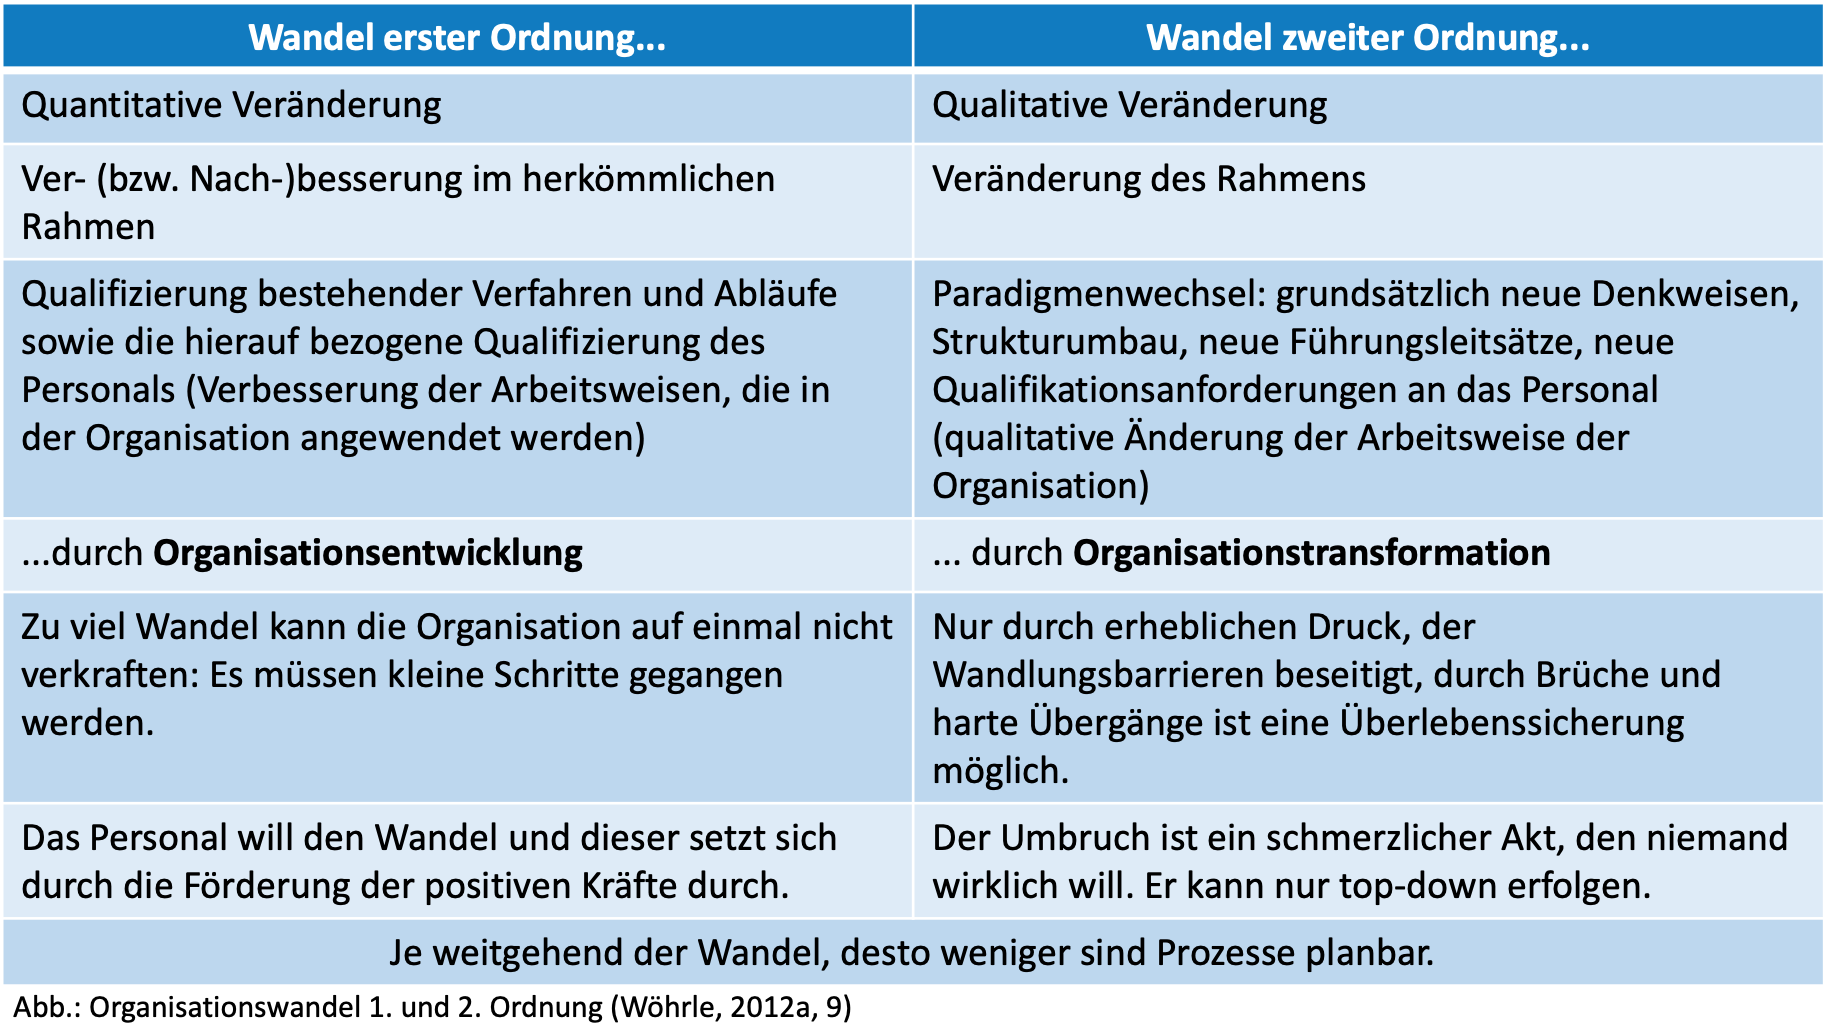
\includegraphics[keepaspectratio]{images/figure313.png}} \hfill{}

\caption{Abb. 3.13: Organisationswandel 1. und 2. Ordnung (nach A.
Wöhrle 2012, S. 9)}

\end{figure}%

In \hyperref[figure313]{Abb. 3.13} zum Kultur- bzw.
Organisationskulturbegriff wurde bereits schon einmal bei der
partizipatorischen Strategie auf die zweite Ordnung eingegangen, welche
nun noch einmal im Detail erläutert wird. Wenn wir einen Wandel zwischen
erster und zweiter Ordnung unterscheiden, dann ist der Wandel in der
ersten Ordnung so etwas wie eine qualitative Veränderung, eine
Optimierung im weitesten Sinne. Wir nehmen Verbesserungen an Strukturen,
Prozessen und an Strategien vor, unter Beachtung der aktuellen
Rahmenbedingungen, denn die Grundsätze und der Zweck der Einrichtung
sind nicht anzutasten. Das kann durch Qualifikation und nach
Qualifikationen der Einrichtungsmitglieder passieren. Verfahren,
Prozesse, Abläufe und Strukturen werden weiterentwickelt,~\emph{ohne die
grundsätzliche Idee, das grundsätzliche Organigramm zu verändern}.
Organisationsentwicklung meint hier im engeren Sinn, dass wir uns auf
der Ebene der ersten Ordnung befinden. Organisationsentwicklung ist ganz
allgemein der Prozess zur Umsetzung von Veränderung. Gleichzeitig hat er
eine zweite Bedeutung inne. Dabei geht es um Veränderungsmaßnahmen, die
der Optimierung dienen und die mit kleinen schrittweisen Veränderungen
einhergehen, sei es durch Politik oder Wandel innerhalb der ersten
Ordnung. Dabei muss letztendlich das Personal mitgenommen bzw. in den
Prozess einbezogen werden sowie regelmäßig motiviert und hinsichtlich
ihrer Ressourcen weiter unterstützt werden.

Mit dem Wandel auf der zweiten Ordnung ist gemeint, dass sich die
Organisation durch~\emph{qualitative}~Veränderung weiterentwickelt und
hierbei nun auch der Rahmen der Einrichtung hinterfragt wird, also die
grundsätzliche Struktur, die grundsätzlichen Missionen der Einrichtung,
die grundsätzlichen Leistungsbereiche.~\emph{Diese werden erweitert oder
gegebenenfalls auch komplett verändert}. Im weiten Sinne findet so etwas
wie ein Paradigmenwechsel statt. Diese Veränderungen führen zu neuen
Denkweisen, zu neuen Strukturen oder zu neuen Leitsätzen. In Folge
dessen muss das Personal an die neuen Rahmenbedingungen angepasst und
(nach)qualifiziert werden. Man spricht dabei auch von einer
Organisationstransformation. Transformation geschieht durch Überwindung
von Barrieren. Dabei werden Brüche innerhalb der Organisation entstehen
und gegebenenfalls auch ein gewisser Handlungsdruck, der von innen und
von außen kommen kann. Dies ist aber für den Wandel in der Organisation
bedeutsam, damit dieser auch in Gang kommen kann und damit letztendlich
das Ziel der Überlebenssicherung dieser Organisation erreicht wird.

Ein Wandel auf der zweiten Ordnung ist dann nicht notwendig, wenn wir
diesen grundsätzlichen Veränderungsprozess nicht angehen und damit das
Überleben bzw. die Existenz der eigenen Einrichtung nicht gesichert ist.
Das kann häufig als schmerzlich oder als Rechtsbruch empfunden werden.
Im Regelfall wird hier meist mit einem Top-Down-Prozess oder einer
Strategie versucht, den Wandel umzusetzen. Wir erkennen zwei
Entwicklungsperspektiven, zwei Extreme: auf der einen Seite die
Organisationsentwicklung im engeren Sinne und auf der anderen Seite die
Transformation. Wir wollen uns in den verschiedenen
Veränderungsprozessen innerhalb der Organisationen entweder auf der
einen Seite sehen oder auf der anderen Seite oder anders ausgedrückt,
innerhalb dieses Kontinuums „von'' „bis'' sehen.

Zur Verdeutlichung helfen folgende Beispiele zur
Organisationsentwicklung im engeren Sinne: Es sind Prozesse gemeint, in
denen wir versuchen -- sei es beispielsweise im Sinne des
Qualitätsmanagements die Optimierung im Ablauf der Eingewöhnungsphase --
die Rahmenbedingungen innerhalb des Tagesablaufs noch einmal anders zu
strukturieren. Oder wir versuchen, Arbeitsverträge an die neuen
Rahmenbedingungen anzupassen. Dies sind Beispiele für die
Organisationsentwicklung erster Ordnung.

Für die Organisationsentwicklung zweiter Ordnung wäre der Einsatz einer
neuen Leitungskraft in einer Einrichtung und der damit einhergehende
neue Anspruch oder die andere Art der Zusammenarbeit beispielhaft. Das
führt gegebenenfalls dazu, dass dadurch neue Prinzipien und Gesetze
erlernt werden müssen oder dass eine Einrichtung erweitert wird oder
dass ein Teil der Einrichtung ausgegliedert wird oder dass zum Beispiel
eine neue Software eingeführt wird. Dies wird von den
Organisationsmitgliedern meist als Bruch erlebt, weil man diesen Wandel
erst einmal in den Alltag integrieren und hier einen viel stärkeren,
tiefgreifenden Veränderungsprozess umsetzen muss.

\section{Ziele der
Organisationsentwicklung}\label{ziele-der-organisationsentwicklung}

Im nachfolgenden Abschnitt beschäftigen wir uns mit den Zielen von
Organisationsentwicklungen, die jeweils verfolgt werden können.
Zusammenfassend kann man sagen, dass die Organisationsentwicklung dazu
dient, die Wirtschaftlichkeit, die Effizienz und die Existenz einer
Einrichtung zu unterstützen. Dies bedeutet, dass Veränderungsprozesse
umgesetzt werden müssen. Es ist das neue „Normal'', dass sich Dinge
verändern. Dies tun wir, um das Überleben der Einrichtung zu sichern.
Insbesondere werden Arbeitsbedingungen und Rahmenbedingungen verändert,
um uns gewissermaßen dem Bedarf anzupassen und letztendlich, um auch die
Qualität der Angebote zu steigern. Darüber hinaus geht
Dokumentationsentwicklung mit Personalentwicklung einher. D. h., jeder
Schritt des Veränderungsprozesses ist auch auf nationaler Ebene zu
denken: Braucht es gegebenenfalls neue Weiterbildungen? Braucht es
vielleicht Umsetzung innerhalb der Einrichtung, um an einem Projekt
beteiligt zu werden? Wie sieht die Motivation im Veränderungsprozess
aus? All das sind Personalentwicklungsfragen. Es dient letztendlich
dazu, die Effektivität dahingehend zu verbessern, dass Innovationen
möglich sind und Lernprozesse stattfinden können. Man kann also von der
sogenannten „lernenden Organisation'' sprechen. Wir betrachten
Veränderungsprozesse als das grundsätzlich Normale und müssen uns
dementsprechend anpassen. D. h., wenn ein neues Qualitätsmanagement
eingeführt wird, eine neue Software eingesetzt wird oder eine neue
Leitungskraft ihre Tätigkeit aufnimmt, dann hat es immer auch etwas mit
dem Lernen und mit der Innovation innerhalb der Einrichtung zu tun.
Letztendlich dient dies aber auch der Bedarfsdeckung und der Erfüllung
von Interessen. Es wird von uns erwartet, dass wir uns als Einrichtung
so weiterentwickeln, dass wir dem Zweck unserer Einrichtung besser
gerecht werden, sodass wir den Bedarf, der sich von unserer Zielgruppe
ableitet und auch durch Stakeholder an uns herangetragen wird,
entsprechend erfüllen.

Wenn wir unseren Blick nach außen wagen, dann ist
Organisationsentwicklung auch damit verbunden, dass wir uns an die
Veränderungen anpassen, die außerhalb der Einrichtung entstehen und die
dazu dienen, Wettbewerbsvorteile zu entwickeln, zu erarbeiten,
nachzuarbeiten oder zu sichern (beispielsweise durch Veränderung der
wirtschaftlichen Rahmenbedingungen oder durch den Wegfall von
Finanzierungsmöglichkeiten oder gesetzliche Änderungen, die entstanden
sind). Dann kann ein organisierter Entwicklungsprozess eingeführt und
eingeleitet werden.

\section{Ebenen der
Organisationsentwicklung}\label{ebenen-der-organisationsentwicklung}

Nachdem wir uns die Ziele und die Formen der Organisationsentwicklung
angeschaut haben, beschäftigen wir uns nun mit den verschiedenen Ebenen
bzw. Dimensionen der Organisationsentwicklung. Nach Kolhoff (2009, S.
10-7) können drei Ebenen unterschieden werden:

\begin{enumerate}
\def\labelenumi{\arabic{enumi}.}
\item
  \emph{Technostrukturebene}: Hiermit ist die technologische bzw. die
  technische Sichtweise auf die Organisationsentwicklung gemeint.
\item
  \emph{Sozialstrukturebene}: Diese strukturelle Sichtweise fragt
  danach, wie das Miteinander, das Zusammenarbeiten in Einrichtungen
  aussieht und welche Systemstruktur es gibt.
\item
  \emph{Systemstrukturebene}: Was macht die Einrichtung im Ganzen aus
  und wie ist die gesamtheitliche Sichtweise auf die Veränderung?
\end{enumerate}

Was bedeutet das jetzt noch einmal im Einzelnen?
Die~\emph{Technostrukturebene}~fragt danach, ob es so etwas wie formale
oder auch schriftliche Regelungen und Normen gibt, wie in der
Einrichtung gearbeitet wird und welche gegebenenfalls weiterentwickelt
werden müssen. Das betrifft zum Beispiel Prozessabläufe oder
Strukturierung in Form von Organigrammen oder festgeschriebene Leitsätze
für die Einrichtung oder Arbeitsverträge und Arbeitsbeschreibungen, die
verändert werden müssen.

Auf der~\emph{Soziostrukturebene}~ist das Zusammenarbeiten bzw. das
Personal innerhalb der Organisation gemeint. So gibt es bspw. beim
Leitbild eine Veränderung, die vorgenommen werden muss oder z. B. haben
die Rentenzusagen Weiterentwicklungsmöglichkeiten für die Mitglieder in
der Organisation geschaffen, also im weitesten Sinne eine
personenorientierte Sichtweise in den Blick genommen.

Auf der~\emph{Systemstrukturebene}~geht es grundsätzlich darum, die
gesamte Einrichtung und ihre Schnittstellen in den Blick zu nehmen. Also
alle Funktionsbereiche, alle Teileinrichtungen des Trägers, welche
gleichzeitig mitbedacht werden müssen, wenn es zu einem
Veränderungsprozess kommen soll. Darüber hinaus betrachten wir uns nicht
nur als Organisation selbst, sondern haben auch immer die
Wechselbeziehung zu unserem System „Umwelt'' -- also die gesetzlichen,
wirtschaftlichen, kooperativen Rahmenbedingungen, die unsere Einrichtung
mit dem System „Umwelt'' verbindet -- im Blick.

Wir müssen nicht immer alle diese drei Ebenen im Rahmen von
Veränderungsprozessen bedienen, aber wir sollten uns im Klaren sein, auf
welcher Ebene wir gerade versuchen, etwas zu verändern. Letztendlich
gibt es auch Wechselbeziehungen zwischen diesen drei Ebenen.

\section{Prozessarchitektur einer
Organisationsentwicklung}\label{prozessarchitektur-einer-organisationsentwicklung}

Wenn wir uns vorstellen, wie der Prozess der Organisationsentwicklung
ablaufen kann oder soll, könnte man versuchen, dies in einer Grafik
darzustellen. Hierfür folgendes Beispiel in \hyperref[figure314]{Abb.
3.14} für eine sogenannte Prozessarchitektur (also die Architektur des
Entwicklungsprozesses) wie es von Schiersmann and Thiel (2014) in ihrem
Buch dargestellt wurde.

\begin{figure}

\pandocbounded{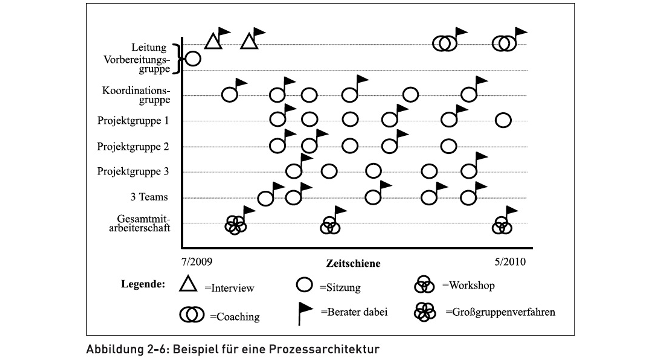
\includegraphics[keepaspectratio]{images/figure314.png}} \hfill{}

\caption{Abb. 3.14: Beispiel für eine Prozessarchitektur (Schiersmann
and Thiel 2014, S. 51)}

\end{figure}%

Es wird, wie in der Legende zu erkennen ist, zwischen unterschiedlichen
Formen der Arbeit im Rahmen der Organisationsentwicklung unterschieden.
Bspw. sind die Interviews als Dreiecke zu erkennen und die Sitzungen
sind als Kreis dargestellt. Es gibt außerdem unterschiedliche andere
Formen, wie zum Beispiel den Workshop im Großgruppenverfahren, wo die
gesamte Belegschaft der Einrichtung zusammenkommt und ein Berater dabei
ist. Wenn sich in der Grafik zwei Kreise überlappen, dann handelt es
sich um Coaching und andere Unterstützungsprozesse. Mit Hilfe der
Legende kann man diese Grafik gut lesen und es wird im Zeitablauf von
circa einem Jahr dargestellt, wo verschiedene Veränderungsmaßnahmen
umgesetzt worden sind. Wie links im Diagramm zu erkennen ist, lassen
sich die Beteiligten in verschiedene Gruppen unterteilen. Es gibt die
Leitung, die einbezogen wird und die ganz am Anfang in der ersten
Sitzung ausfindig machen muss, wo der Bedarf für den Veränderungsprozess
ist. Folglich wird mit den Beratern der Auftrag zum Veränderungsprozess
und die Methodik besprochen und gleichzeitig eine Koordinationsgruppe
einberufen. Trotzdem muss am Anfang (oder nachdem der Auftrag erklärt
worden ist) die gesamte Mitarbeiterschaft mit angesprochen und darüber
informiert werden, wo wir uns gerade in dem Prozess befinden. Über den
Prozessverlauf hin, also über die verschiedenen Monate die folgen, gibt
es sowohl auf Teamebene als auch auf Projektgruppenebene verschiedene
Ereignisse, die umgesetzt werden, wo nach Veränderungen geschaut und
entsprechend Lösungen entwickelt werden. Das geschieht hier auf Basis
der Projektarbeit in den verschiedenen Gruppen. Es sind Sitzungen,
welche teils mit einem Berater durchgeführt werden,
Großgruppenveranstaltungen und Workshops, die geplant sind und im
Veränderungsprozess stattfinden. Am Ende des Prozesses finden wir auf
der Leitungsebene verschiedene Coachingprozesse, die durchgeführt
werden, um die Leitung dabei zu unterstützen, Konsequenzen aus den
Erkenntnissen zu ziehen und die neuen Veränderungen verbindlich zu
machen. Die Leitung wird befähigt, Bericht gegenüber der Belegschaft zu
erstatten, was zukünftig verändert werden muss. Was wir auch erkennen
können ist, dass die Koordinationsgruppe -- das ist die zweite Ebene von
oben gesehen -- an ganz unterschiedlichen Stellen während des gesamten
Prozesses die Aufgabe hat, die verschiedenen Teams anzuleiten und
letztendlich auch die Ergebnisse der einzelnen Projektgruppen
zusammenzutragen, um diese dann zusammenzufassend der Leitung zu
übergeben bzw. mit der Leitung zu diskutieren.

Der hier dargestellte Prozess sieht relativ komplex aus, ist aber kein
extravagantes Beispiel und sehr stark an die Praxis angelehnt. Er zeigt
ganz deutlich, wie viele verschiedene Kommunikationspunkte und
Austauschbeziehungen es gibt und wie viele Sitzungen es geben muss, um
so einen Entwicklungsprozess sinnvoll ablaufen zu lassen. Dieses
Beispiel diente dazu, um uns einen Überblick zu verschaffen, wie man
solch einen Prozess gestalten kann, der partizipativ orientiert ist und
der stark auf die Arbeit in Projektgruppen ausgerichtet ist.

\section{Modelle der
Organisationsentwicklung}\label{modelle-der-organisationsentwicklung}

\subsection{Überblick}\label{uxfcberblick}

Nachdem wir von den Zielen und Formen sowie von den verschiedenen Ebenen
und dem Prozess von Organisationsentwicklung gesprochen haben, werden
wir uns nun verschiedene Ansätze, Konzepte und Modelle anschauen. Dazu
werden wir uns vorerst drei klassische Ansätze ansehen und einen
weiterführenden Ansatz besprechen.

Zunächst ist die~\emph{Feldtheorie von Kurt Lewin}~zu nennen. Darin geht
es um die Frage, wie man so etwas wie förderliche und nichtförderliche
Faktoren im Rahmen der Organisationsentwicklung unterscheiden,
herausfinden und entsprechend einsetzen kann.

Die~\emph{Aktionsforschung}~beschäftigt sich damit, wie wir forschen,
lernen und Praxisveränderungen gemeinsam entdecken können. Es ist
gewissermaßen ein Spiel zwischen Praxis und Theorie.

Das~\emph{Drei-Phasen-Modell von Kurt Lewin}~-- welches wir uns bereits
am Anfang des Semesters in den Grundlagen angeschaut haben -- beinhaltet
drei Phasen des Veränderungsprozesses, nämlich die Phasen Unfreezing --
Moving -- Refreezing.

Mit den neueren Modellansätzen, zu denen beispielsweise die lernende
Organisation gehört, werden wir uns im Rahmen der Organisationskultur
bzw. in den entsprechenden Seminaren beschäftigen. Letztendlich gibt es
verschiedene weitere Ansätze zu nennen, obwohl dieser einer der
bekanntesten ist.

Des Weiteren ist im Rahmen der Organisationsentwicklung der systemische
Ansatz relevant, bei dem es darum geht, die gesamte Einrichtung zu
betrachten. Dabei geht es nicht darum, einzelne Personen verantwortlich
und haftbar zu machen, dass Veränderungsprozesse umgesetzt werden,
sondern dass wir immer jede Veränderung aus der Perspektive der gesamten
Einrichtung denken müssen. Wenn Veränderung in einem Bereich
stattfindet, bedeutet dies, dass es auch Auswirkung auf einen anderen
Bereich hat. Das wäre ebenfalls beispielsweise einer der neueren
Ansätze. Darüber hinaus gibt es eine ganze Reihe von kundenspezifischen
Ansätzen, die sich in den letzten zwei, drei Jahrzehnten intensiv
entwickelt haben.

\subsection{Feldtheorie nach Kurt
Lewin}\label{feldtheorie-nach-kurt-lewin}

Beschäftigen wir uns nun mit dem ersten Modell der
Organisationsentwicklung, der Feld-Theorie nach Kurt Lewin. Kurt Lewin
war ein bekannter Psychologe im 20. Jahrhundert, der sich mit
verschiedenen Ansätzen beschäftigt hat, beispielsweise der Kraft- oder
Kräftefeld-Theorie. Was ist damit gemeint? Damit ist gemeint, dass
einerseits das Verhalten von uns Menschen als auch andererseits wir uns
als Person entwickeln und unsere Beziehung zur Umwelt durch verschiedene
Kräfte beeinflusst werden können, die positiv, aber auch negativ sein
können. Ein Beispiel für positive Kräfte wäre, wenn wir zum Beispiel
Hunger haben und das Bedürfnis verspüren, etwas zu uns zu nehmen. Wir
essen dann etwas (als Energielieferant) und erhalten durch diese
positive Kraft (durch Energiezufuhr) die Möglichkeit, unser Bedürfnis zu
befriedigen. Wenn man diese positive Kraft auf Organisationen überträgt,
dann geht es am Anfang darum, ein Problem zu analysieren und
herauszufinden, wo etwas stört bzw. wo etwas verändert werden muss, um
daraus dann Fragen ableiten zu können, wie beispielsweise: Was gibt es
für Faktoren, die den Veränderungsprozess unterstützen können? Das ist
in der Feld-Theorie im Rahmen der Organisationsentwicklung beschrieben.
Zusammengefasst bedeutet es, dass die menschliche Entwicklung in unserem
Handeln sowie die zwischenmenschlichen Beziehungen in der Gesamtheit ein
strukturiertes und dynamisches Feld darstellen. Durch verschiedene
Kräfte, die immer auf das eine und das andere wirken, kommt es zu
Veränderungen. Man kann sagen, das ganze Leben ist eine Veränderung.
Unsere gesamte menschliche Entwicklung ist Veränderung.

\begin{figure}

\pandocbounded{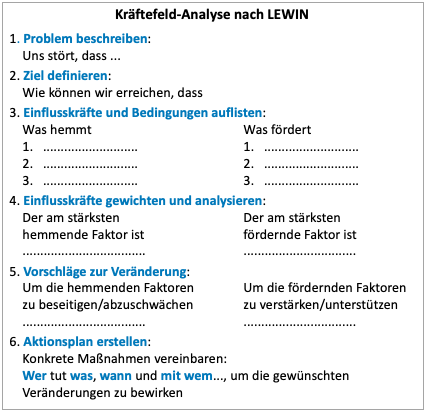
\includegraphics[keepaspectratio]{images/figure315.png}} \hfill{}

\caption{Abb. 3.15: Kräfte-Analyse von Lewin (nach Becker \& Langosch,
2002, zit n. Kolhoff 2009, S. 23)}

\end{figure}%

In \hyperref[figure315]{Abb. 3.15} ist ein Kräftefeld dargestellt. Die
Kräftefeld-Analyse hat einen Stufenplan, den man durcharbeiten kann.
Dies ist hilfreich für die praktische Planung von
Organisationsentwicklungen. Am Anfang versucht man, das Problem zu iben.
Man erfasst, was stört bzw. was verändert werden muss und leitet daraus
seine Zielstellung ab. Was wollen wir erreichen? Was wollen wir
verändern? Dann kann man überlegen, welche Kräfte es gibt und welche
Rahmenbedingungen sich auf das Erreichen der Ziele auswirken -- entweder
hemmend oder fördernd. Wenn wir die Einflusskräfte -- positiv wie
negativ -- anschließend isoliert haben, können wir nun versuchen, diese
zu gewichten und zu priorisieren, was wie angegangen werden soll. Im
fünften Schritt machen wir uns nun Gedanken darüber, welche Maßnahmen
gegebenenfalls geeignet sind und welche Vorschläge es gibt, diese
Veränderung zu bewirken, beispielsweise wie hemmende Faktoren eventuell
beseitigt oder abgeschwächt werden können oder wie fördernde Faktoren
gestärkt und noch weiter unterstützt werden können. Daraus erstellen wir
als sechsten Schritt einen Aktionsplan, der über die Maßnahmen, die
Verantwortlichkeiten, den Zeitpunkt und die Teilziele informiert. Z. B.,
wer macht was, um die gewünschte Veränderung zu bewirken. Das ist ein
relativ einfaches, aber sehr praktikables Modell, um die
Organisationsentwicklung umzusetzen.

\subsection{Aktionsforschung}\label{aktionsforschung}

Im Rahmen der Aktionsforschung beeinflussen sich Veränderungen und das
Handeln der Betroffenen in einer Organisation gegenseitig. Die Forschung
dient dazu, das Handeln und die Betroffenen in Einrichtungen zu
unterstützen bzw. Anleitung zu geben, wie der Veränderungsprozess
bewältigt werden kann. Dabei werden unterschiedliche Rollen eingenommen
-- wie die Forscher*innen, die jeweils agierenden Betroffenen der
Einrichtungen und die Personen, die den Prozess beobachten -- weil
einerseits die Forschenden gleichzeitig auch als Praktiker unterwegs
sind und Dinge innerhalb der Organisation verändern und Aktionen
umsetzen und andererseits auch die Beteiligten in Organisationen den
Prozess mit erforschen, indem sie reflektieren, was die Veränderung ist
und welche Veränderungen bewirkt werden sollen. Wir können davon
ausgehen, dass dabei verschiedene Prozesse parallel stattfinden, also
Forschen in dem Sinne, dass wir versuchen herauszufinden, wie die
aktuelle Situation ist. Erst dann können wir die Situation verändern, in
dem wir Ziele setzen. Kurz zusammengefasst heißt das: Auf Basis dieser
Forschung kommt es zu Veränderungen in der Praxis, die letztendlich zu
Verbesserungen führen sollen, nämlich wie wir lernen, wie die
Organisationen sich weiterentwickeln können, wie wir Innovationen
umsetzen und wie das letztendlich wieder der Ausgangspunkt für einen
erneuten Start dieses Prozesses sein kann (vgl.
\hyperref[figure316ux5cux255D]{Abb. 3.16}).

\begin{figure}

\pandocbounded{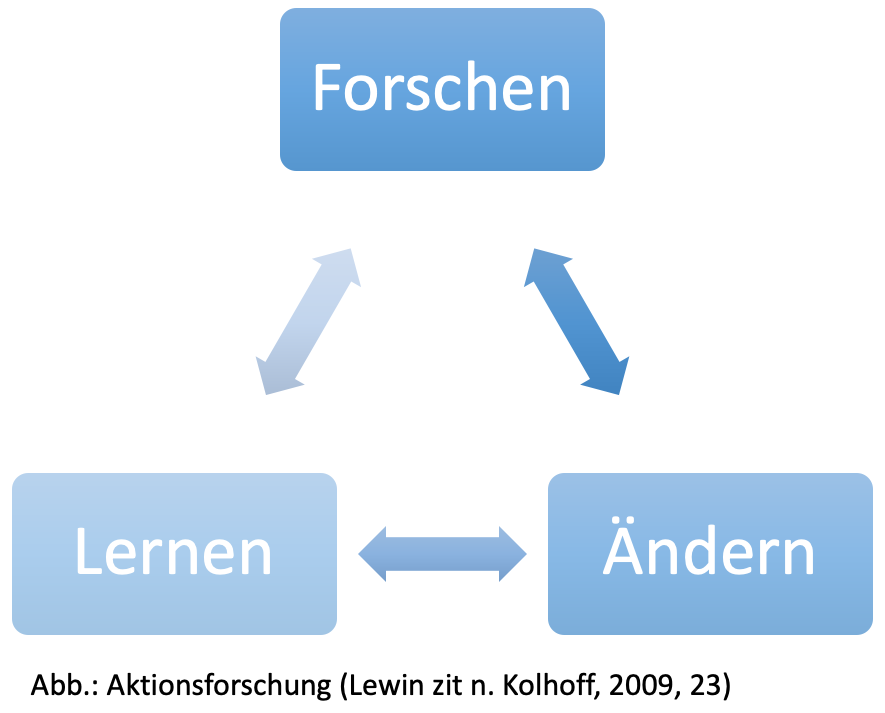
\includegraphics[keepaspectratio]{images/figure316.png}} \hfill{}

\caption{Abb. 3.16: Aktionsforschung (nach Lewin zit n. Kolhoff 2009, S.
23)}

\end{figure}%

Das Dreieck symbolisiert einen Kreislauf. Forschung ist Ausgangspunkt,
wurde selbst zum Forschungsgegenstand und kann hinterfragt werden: (1)
Haben wir die Ziele erreicht und (2) was muss vielleicht zukünftig noch
entwickelt werden, weil sich beispielsweise die Rahmenbedingungen schon
wieder geändert haben? Das Modell zeigt, dass sich die forschende
Haltung, die Änderungshaltung und das kontinuierliche Lernen beständig
abwechseln. Dabei handelt es sich um ein theoretisches Modell, welches
einfach in der Praxis umgesetzt werden kann. Im Rahmen einer
Abschlussarbeit über einen Veränderungsprozess innerhalb einer
Einrichtung können wir dokumentieren und retrospektiv herausfinden, wie
umgesetzt wurde. Daraus können wir ein Konzept entwickeln und gehen mit
diesem in die Einrichtung. In der Einrichtung finden wir die
Mitwirkenden vor, die den Änderungsprozess umsetzen, die das Feld ändern
und gleichzeitig in der Organisation lernen. In einer anschließenden
Evaluation oder Reflexion können die Mitwirkenden ausfindig machen, was
innerhalb der Einrichtung zu einer Veränderung geführt hat bzw. welche
Faktoren sich in der Einrichtung verändert haben. Im weiteren Sinne
handelt es sich hierbei um eine Handlungsforschung, die wir mit unserer
Abschlussarbeit betreiben würden, da wir ein Konzept entwickeln, dieses
Konzept umsetzen und hinterher überprüfen, ob dieses tatsächlich
sinnvoll umgesetzt werden konnte.

\subsection{Dreiphasen-Modell der Organisationsentwicklung nach Kurt
Lewin}\label{dreiphasen-modell-der-organisationsentwicklung-nach-kurt-lewin}

Im~\emph{Drei-Phasen-Modell von Kurt Lewin}~werden drei
Entwicklungsphasen unterschieden (vgl. \hyperref[figure317]{Abb. 3.17}).

\begin{figure}

\pandocbounded{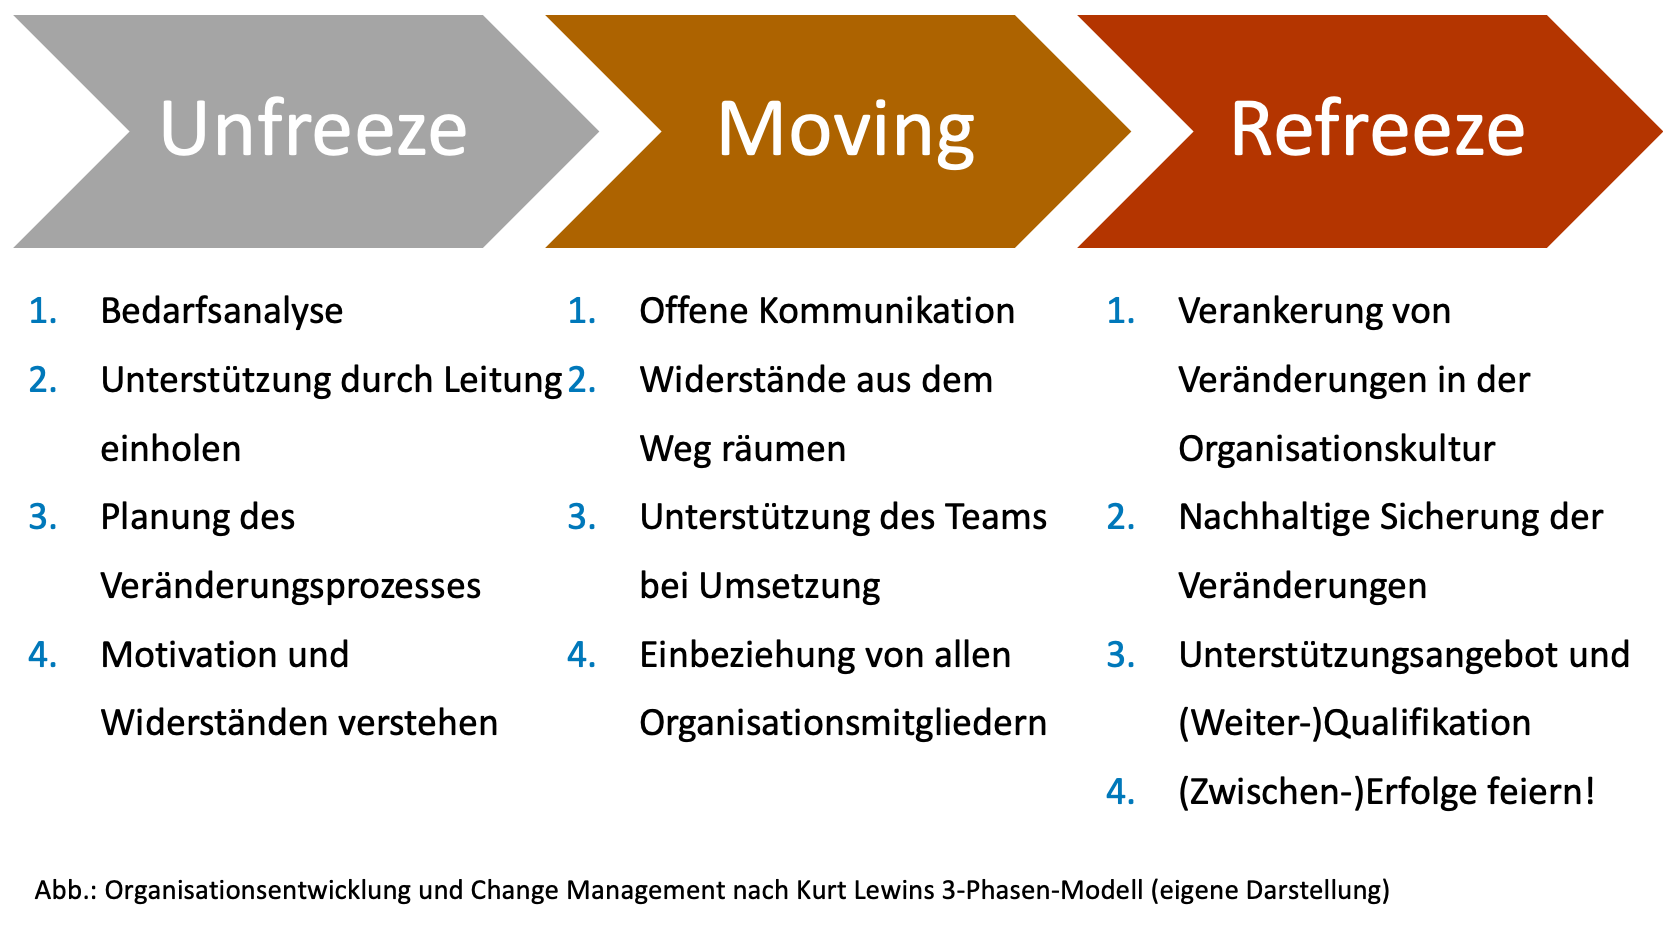
\includegraphics[keepaspectratio]{images/figure317.png}} \hfill{}

\caption{Abb. 3.17: Organisationsentwicklung und Change-Management nach
Kurt Lewins 3-Phasen-Modell (eigene Darstellung)}

\end{figure}%

Kurz zur Begrifflichkeit: Beim~\emph{Unfreezing}~(1. Phase) geht es
darum, die bisherigen Strukturen zu analysieren und in Frage zu stellen.
Dabei geht es darum, Veränderungen umzusetzen, Maßnahmen dafür zu
ergreifen und Aktionen zu planen.~\emph{Refreezing}~(2. Phase) bedeutet
in diesem Modell „etwas verbindlich machen'' oder „einfrieren''. Dabei
erfolgt das „Einfrieren'' der neu gefundenen Strukturen, Prozesse und
Abläufe, mit anderen Worten eine Verbindlichmachung und Legitimation der
Veränderungen.

Im~\emph{Unfreezing}~(1. Phase) geht es auch darum, den Bedarf zu
ermitteln. Durch die Einrichtungsleitung muss auch Unterstützung
eingeholt werden, weil Veränderungsprozesse grundsätzlich einfach dann
gut funktionieren, wenn die Leitung dahintersteht und über sie die
Veränderung gegebenenfalls eingefordert werden kann. Des Weiteren muss
der Veränderungsprozess vorbereitet werden, die Methodik muss
abgesprochen werden, der Zeitraum sowie die dafür zur Verfügung
stehenden Ressourcen (Personalressourcen und Sachressourcen) müssen
geplant werden und schließlich geht es darum, über die Veränderungen
erst einmal zu informieren und bei Widerständen bzw. bei auftretenden
Fragen entsprechend zu motivieren und den Veränderungsprozess
verständlich zu machen und zu erklären, warum wir uns in diese
Veränderung hinein begeben werden.

Beim~\emph{Moving}~(2. Phase) geht es schließlich darum, Aktionen und
Maßnahmen zu planen, um dann die Veränderung zu bewirken. Hier gilt es
Prinzipien einzuhalten, wie z. B., dass offen kommuniziert wird, dass
regelmäßig informiert wird und dass alle an dem Vorhaben beteiligt
werden. Es gilt, aktiv zu kommunizieren, Widerstände zu bearbeiten und
aus dem Weg zu räumen. Meistens lassen sich nicht alle Widerstände aus
dem Weg räumen und man muss versuchen, möglichst alle im Team bzw. in
der Einrichtung anzusprechen und zu beteiligen, damit der
Veränderungsprozess erfolgreich umgesetzt werden kann. Wir müssen die
Unterstützung im Team suchen bzw. -- und das haben wir vorhin bei der
Prozessbeschreibung von Organisationsentwicklung schon gesehen --
einzelne Projektgruppen oder Teams mit Aufgabenstellungen betrauen, um
hierfür dann Lösungen zu suchen. Darüber hinaus geht es darum,
Organisationsmitglieder einzubeziehen und Partizipation zu erleben.

Im abschließenden~\emph{Unfreezing}~(3. Phase) geht es um das
Verbindlichmachen der neu gefundenen Strukturen, Prozesse und
kulturellen Überzeugungen. Es geht darum, diese zu verankern und
maßgeblich die Organisationskultur weiterzuentwickeln. Hier geht die
Organisationsentwicklung mit der Entwicklung der Organisationskultur
einher (vgl. Abschnitt 2.4). Wichtig ist auch die nachhaltige Sicherung
der Veränderung, dass man die Dinge, die man verändern hat, festschreibt
bzw. gegebenenfalls eine Dienstvereinbarung daraus entwickelt und als
den neuen „Status quo'' festgelegt. Es werden auch
Unterstützungsnotwendigkeiten angesprochen, bspw. für eine
Weiterqualifikation, um damit weiterarbeiten zu können. Zum Schluss
schließlich sollte jede einzelne Phase, jeder einzelne Prozessschritt
auch gefeiert werden. Diesen dreiphasigen Prozess kann man auch als eine
Art Kreislaufsystem betrachten, der immer wieder abläuft und der sich in
verschiedenen Phasen auch fortentwickelt.

\subsection{Fazit}\label{fazit}

Die drei vorgestellten klassischen Modelle kann man wie folgt
zusammenfassen: Es gibt im Regelfall drei Phasen, die im Rahmen der
Organisationsentwicklung mitbedacht werden sollen. Am Anfang steht die
Phase der~\emph{Diagnose}. In dieser verschaffen wir uns einen Überblick
über den Ist-Stand. In der zweiten Phase versuchen wir,~\emph{Maßnahmen
der Veränderung umzusetzen}~und dementsprechend auch einen neuen „Status
quo'' zu erreichen. Und schließlich -- drittens -- ist es die Aufgabe
der Leitung bzw. aller Einrichtungsmitglieder und Führungskräfte dafür
zu sorgen, dass die neu gefundenen Aufgaben, Prozesse, Strukturen
entsprechend umgesetzt werden bzw. zukünftig als~\emph{verbindlich
legitimiert} werden.

\part{Anhang}

\chapter{Literaturverzeichnis}\label{literaturverzeichnis}

\phantomsection\label{refs}
\begin{CSLReferences}{1}{0}
\bibitem[\citeproctext]{ref-Arnold2022b}
Arnold, Maik. 2022a. {``Hybrid Function of Social Work Management
Education.''} figshare.
\url{https://doi.org/10.6084/M9.FIGSHARE.20079650.V1}.

\bibitem[\citeproctext]{ref-Arnold2022a}
---------. 2022b. {``{Social Work Management Subject Map},''} June.
\url{https://doi.org/10.6084/m9.figshare.20151839.v1}.

\bibitem[\citeproctext]{ref-arnold2019Finanzbuchhaltunga}
---------. 2024. {``Finanzbuchhaltung.''} In \emph{Das große Handbuch
Organisation und Verwaltung in der Kita}, edited by Harald Christa, 2nd
ed., 243--64. Köln: Carl Link.

\bibitem[\citeproctext]{ref-Arnold_Bonchino-Demmler_Evers_Hussmann_Liedke_2017}
Arnold, Maik, Dorothy Bonchino-Demmler, Ralf Evers, Marcus Hußmann, and
Ulf Liedke. 2017. \emph{Perspektiven Diakonischer Profilbildung: Ein
Arbeitsbuch Am Beispiel von Einrichtungen Der Diakonie in Sachsen}.
Leipzig: Evangelische Verlagsanstalt.

\bibitem[\citeproctext]{ref-bachmann2008}
Bachmann, P. 2008. \emph{Grundlagen Des Controlling in Sozialen
Organisationen}. 2. Aufl. Brandenburg: Hochschulverbund Distance
Learning (HDL Nr. 2-020-2601).

\bibitem[\citeproctext]{ref-Bate2010}
Bate, S. Paul. 2010. \emph{Strategies for Cultural Change}. Routledge.
\url{https://doi.org/10.4324/9780080517971}.

\bibitem[\citeproctext]{ref-Beck2013}
Beck, Reinhilde, Klaus Grunwald, Klaus Schellberg, Gotthart Schwarz,
Wolf Rainer Wendt, and Armin Wöhrle. 2013. {``Kapitel 1
Sozialwirtschaft.''} In \emph{Grundlagen Des Managements in Der
Sozialwirtschaft}, 11--34. Nomos Verlagsgesellschaft mbH \& Co. KG.

\bibitem[\citeproctext]{ref-Boessenecker2014}
Boeßenecker, Karl-Heinz, and Andreas Markert. 2014. \emph{Studienführer
Sozialmanagement}. Nomos. \url{https://doi.org/10.5771/9783845250915}.

\bibitem[\citeproctext]{ref-Brinkmann2010}
Brinkmann, Volker. 2010. \emph{Sozialwirtschaft}. Gabler.
\url{https://doi.org/10.1007/978-3-8349-8935-2}.

\bibitem[\citeproctext]{ref-Bundesagentur2014beschaeftigte}
Bundesagentur für Arbeit Berichte. 2014/2020. {``Beschäftigte Nach
Wirtschaftszweigen (WZ 2008) (Monatszahlen).''}
\url{https://statistik.arbeitsagentur.de/Statistikdaten/Detail/202007/iiia6/beschaeftigung-sozbe-monatsheft-wz/monatsheft-wz-d-0-202007-pdf.pdf?__blob=publicationFile&v=1}
(2020),
\url{https://statistik.arbeitsagentur.de/Statistikdaten/Detail/201409/iiia6/beschaeftigung-sozbe-monatsheft-wz/monatsheft-wz-d-0-201409-pdf.pdf?__blob=publicationFile&v=1}
(2014).

\bibitem[\citeproctext]{ref-Christa2010}
Christa, Harald. 2010. \emph{Grundwissen Sozio-Marketing}. VS Verlag für
Sozialwissenschaften. \url{https://doi.org/10.1007/978-3-531-92438-0}.

\bibitem[\citeproctext]{ref-Europeancommission2015social}
European Commission. 2015. {``The Social Business Initiative of the
European Commission.''}
\url{http://ec.europa.eu/DocsRoom/documents/14583}.

\bibitem[\citeproctext]{ref-Evers2010}
Evers, Adalbert, and Benjamin Ewert. 2010. {``Hybride Organisationen Im
Bereich Sozialer Dienste. Ein Konzept, Sein Hintergrund Und Seine
Implikationen.''} In \emph{Soziale Personenbezogene
Dienstleistungsorganisationen}, 103--28. VS Verlag für
Sozialwissenschaften. \url{https://doi.org/10.1007/978-3-531-92474-8_4}.

\bibitem[\citeproctext]{ref-Giesel2007-jy}
Giesel, Katharina D. 2007. \emph{Leitbilder in Den
Sozialwissenschaften}. 2007th ed. Vs Verlag Fur Sozialwissenschaften.

\bibitem[\citeproctext]{ref-Graf2013-rq}
Graf, Pedro, and Maria Spengler. 2013. \emph{Leitbild- Und
Konzeptentwicklung}. 6th ed. Augsburg, Germany: ZIEL.

\bibitem[\citeproctext]{ref-Groysberg_Lee_Price_Chen_2018b}
Groysberg, Boris, Jeremiah Lee, Jesse Price, and J. Yo-Jud Chen. 2018a.
{``Eine Frage Der Kultur.''} \emph{Harvard Business Manager}, no. 3:
20--31.

\bibitem[\citeproctext]{ref-Groysberg_Lee_Price_Chen_2018a}
---------. 2018b. {``The Leader's Guide to Corporate Culture: How to
Manage the Eight Critical Elements of Organizational Life.''}
\emph{Harvard Business Review} 98 (1): 44--52.

\bibitem[\citeproctext]{ref-helmig2019nonprofit}
Helmig, B. 2019. {``Nonprofit-Organisation (NPO).''} In \emph{Gabler
Wirtschaftslexikon}.
\url{https://wirtschaftslexikon.gabler.de/definition/nonprofit-organisation-npo-39562}.

\bibitem[\citeproctext]{ref-holzle2006}
Hölzle, C. 2006. \emph{Personalmanagement in Einrichtungen Der Sozialen
Arbeit: Grundlagen Und Instrumente}. Weinheim, München: Juventa.

\bibitem[\citeproctext]{ref-IDW2004wohlfahrtsverbaende}
Institut der Deutschen Wirtschaft Köln, ed. 2004.
\emph{Wohlfahrtsverbände in Deutschland: Auf Den Schultern Der
Schwachen}. Dt. Instituts-Verlag.
\url{https://www.yumpu.com/de/document/view/7199735/auf-den-schultern-der-schwachen}.

\bibitem[\citeproctext]{ref-Karmann2011gutachten}
Karmann, A., A. Werblow, B. Karmann, and A. Jurack. 2011. {``Gutachten
Zur Sozialwirtschaft in Sachsen Unter Besonderer Berücksichtigung Der
Freien Wohlfahrtspflege.''} Liga der Freien Wohlfahrt Sachsen.
\url{https://tu-dresden.de/bu/wirtschaft/wwsprofecon/ressourcen/dateien/publikationen/Sozialwirtschaft_2011.pdf?lang=de}.

\bibitem[\citeproctext]{ref-Klatetzki2010}
Klatetzki, Thomas. 2010. {``Zur Einführung: Soziale Personenbezogene
Dienstleistungsorganisation Als Typus.''} In \emph{Soziale
Personenbezogene Dienstleistungsorganisationen}, 7--24. VS Verlag für
Sozialwissenschaften. \url{https://doi.org/10.1007/978-3-531-92474-8_1}.

\bibitem[\citeproctext]{ref-kolhoff2005}
Kolhoff, L. 2005. \emph{Organisationsanalyse}. 2. Aufl. Hochschulverband
Distance Learning (HDL Nr. 2-020-1201).

\bibitem[\citeproctext]{ref-kolhoff2009}
---------. 2009. \emph{Ziele, Modelle Und Methoden Der
Organisationsentwicklung}. 2. Aufl. Hochschulverband Distance Learning
(HDL Nr. 2-020-1202).

\bibitem[\citeproctext]{ref-Lambers2015-el}
Lambers, Helmut. 2015. \emph{Management in Der Sozialen Arbeit Und in
Der Sozialwirtschaft}. Grundlagentexte Soziale Berufe. Weinheim,
Germany: Juventa Verlag ein Imprint der Julius Beltz.

\bibitem[\citeproctext]{ref-Liedke_2017}
Liedke, Ulf. 2017. {``Diakonische Profilentwicklung Als Teil Der
Organisationentwicklung.''} In \emph{Perspektiven Diakonischer
Profilentwicklung. Ein Arbeitsbuch Am Beispiel von Einrichtungen Der
Diakonie in Sachsen}, edited by Maik Arnold, Dorothy Bonchino-Demmler,
Ralf Evers, Marcus Hussmann, and Ulf Liedke, 105--250. Leipzig: EVA.

\bibitem[\citeproctext]{ref-Maak2007-vs}
Maak, Thomas, and Peter Ulrich. 2007. \emph{Integre
Unternehmensf{ü}hrung}. 1st ed. Stuttgart, Germany: Sch{ä}ffer-Poeschel.

\bibitem[\citeproctext]{ref-Morgan1986-oj}
Morgan, Gareth. 1986. \emph{Images of Organization}. 1st ed. Thousand
Oaks, CA: SAGE Publications.

\bibitem[\citeproctext]{ref-Morgan2006-tj}
---------. 1997. \emph{Bilder Der Organisation}. 1st ed. Stuttgart,
Germany: Klett-Cotta.

\bibitem[\citeproctext]{ref-Mross2017}
Mroß, Michael. 2017. {``Leistungsentgelt in Der Sozialwirtschaft.''}
\emph{Blätter Der Wohlfahrtspflege} 164 (6): 225--27.
\url{https://doi.org/10.5771/0340-8574-2017-6-225}.

\bibitem[\citeproctext]{ref-Muller-Scholl1992-bt}
Müller-Schöll, Albrecht, and Manfred Priepke. 1992.
\emph{Sozialmanagement}. 3rd ed. K{ö}ln, Germany: Hermann Luchterhand
Verlag.

\bibitem[\citeproctext]{ref-Ribbeck2020-vk}
Ribbeck, Jochen. 2020. \emph{Personalmanagement in Sozialunternehmen}.
WALHALLA Fachverlag.

\bibitem[\citeproctext]{ref-Ritter-Mamczek2016}
Ritter-Mamczek, Bettina. 2016. \emph{Stoff Reduzieren}. Kompetent
Lehren. Stuttgart, Germany: UTB.

\bibitem[\citeproctext]{ref-Ruegg-Sturm2003-ga}
Rüegg-Stürm, Johannes. 2003. \emph{Das Neue St. Galler
{Management-Modell}}. 2nd ed. Bern, Switzerland: Haupt Verlag.

\bibitem[\citeproctext]{ref-Schedler2013multirationales}
Schedler, Kuno, and Johannes Rüegg-Stürm. 2013. \emph{Multirationales
Management: Der Erfolgreiche Umgang Mit Widerspr{ü}chlichen
Anforderungen an Die Organisation}. Haupt.

\bibitem[\citeproctext]{ref-Schiersmann2014}
Schiersmann, Christiane, and Heinz-Ulrich Thiel. 2014.
\emph{Organisationsentwicklung: Prinzipien Und Strategien von
Veränderungsprozessen}. Springer Fachmedien Wiesbaden.
\url{https://doi.org/10.1007/978-3-658-03485-6}.

\bibitem[\citeproctext]{ref-Schreygg2016}
Schreyögg, Georg, and Daniel Geiger. 2016. \emph{Organisation:
Grundlagen Moderner Organisationsgestaltung. Mit Fallstudien}. Springer
Fachmedien Wiesbaden. \url{https://doi.org/10.1007/978-3-8349-4485-6}.

\bibitem[\citeproctext]{ref-Schwarz1986management}
Schwarz, P. 1986. \emph{Management in Nonprofit-Organisationen:
{Ö}ffentliche Verwaltungen Und Betriebe, Verb{ä}nde, Vereine, Parteien,
Kirchen, Sozialwerke}. Schweizer Volksbank.

\bibitem[\citeproctext]{ref-Thommen2000-kd}
Thommen, Jean-Paul. 2000. \emph{Managementorientierte
Betriebswirtschaftslehre}. 6th ed. Managementorientierte
Betriebswirtschaftslehre. Z{ü}rich, Switzerland: Versus.

\bibitem[\citeproctext]{ref-woehrle2001}
Wöhrle, A. 2001. \emph{Organisationswandel Als Kulturwandel}. 2. Aufl.
Brandenburg: Hochschulverband Distance Learning (HDL Nr. 2-020-1102).

\bibitem[\citeproctext]{ref-woehrle2012a}
---------. 2012. \emph{Organisationen Als Reformresistente Gebilde}. 2.
Aufl. Hochschulverband Distance Learning (HDL Nr. 2-020-1101).

\bibitem[\citeproctext]{ref-Whoerle2007}
Wöhrle, Armin. 2007. {``Synergielösungen Für Sozialräume.''}
\emph{Blätter Der Wohlfahrtspflege} 154 (4): 153--55.
\url{https://doi.org/10.5771/0340-8574-2007-4-153}.

\bibitem[\citeproctext]{ref-Wohrle2017}
---------. 2017. {``25 Jahre Sozialmanagement -- Ein Kritischer
r{ü}ckblick.''} In \emph{Gegenwart Und Zukunft Des Sozialmanagements Und
Der Sozialwirtschaft}, 7--34. Wiesbaden: Springer Fachmedien Wiesbaden.

\end{CSLReferences}


\backmatter


\end{document}
